% Created 2012-02-27 Mo 15:39
\documentclass[11pt]{scrartcl}
\usepackage[utf8]{inputenc}
\usepackage[T1]{fontenc}
\usepackage{fixltx2e}
\usepackage{graphicx}
\usepackage{longtable}
\usepackage{float}
\usepackage{wrapfig}
\usepackage{soul}
\usepackage{textcomp}
\usepackage{marvosym}
\usepackage{wasysym}
\usepackage{latexsym}
\usepackage{amssymb}
\usepackage{hyperref}
\tolerance=1000
\providecommand{\alert}[1]{\textbf{#1}}

\title{Sskresztas Gedächtniskristall}
\author{Arne Babenhauserheide}
\date{\today}
\hypersetup{
  pdfkeywords={},
  pdfsubject={},
  pdfcreator={Emacs Org-mode version 7.8.03}}

\begin{document}

\maketitle

\section{Sskresztas Gedächtniskristall}

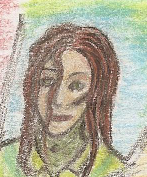
\includegraphics{sskreszta-portrait-alt-klein.png}Aufzeichnungen
von
\href{http://1w6.org/deutsch/kampagnen/w-chter-der-zeit/charaktere/sskreszta}{Sskreszta}
{[}1{]}, Raumpilotin und Psionikerin aus der alten Zeit, die nach 6.000
Jahren aus Ihrer Kryokapsel erwachte.

\begin{quote}
\textbf{» \href{http://1w6.org/print/book/export/html/59}{Chronologische
Druckversion} {[}2{]} «}

\end{quote}
Einträge an denen ich gerade schreibe und noch nicht ausreichend
überarbeitete frühere Aufzeichnungen stehen auf einer
\href{http://1w6.org/rpg\_logs/sskreszta/index.html}{statischen Seite}
{[}3{]}, bis ich sie hochlade (kommt direkt aus der Versionsverwaltung).
Eine wichtige Nebenhandlung ist
\href{http://1w6.org/deutsch/welten/raumzeit/geschichten/piraten-und-zerg}{Piraten
und Zat} {[}4{]}.

Die Einträge gibt es auch
\href{http://1w6.org/stichwort/sskreszta-log}{im Weblog Format} {[}5{]}
- inklusive \href{http://1w6.org/stichwort/sskreszta-log/feed}{RSS-feed}
{[}6{]}.

\section{Der Anfang (Kapitel)}

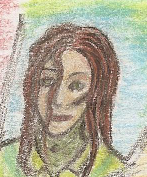
\includegraphics{sskreszta-portrait-alt-klein.png}\emph{Wie
unsere Reisen begannen\ldots{} Wir haben viel erlebt und die Erinnerung
an unsere Abenteuer ist mir ein wertvoller Schatz. Hier sammle ich daher
etwas überarbeitet die Erinnerungen, die Sskreszta während unserer
ersten Jahre in ihrem Gedächtniskristall gespeichert hat - vom Anfang
unserer Reise bis hin zur Piratenjagd.}

Sie werden Stück für Stück eingefügt, sowie ich sie überarbeiten kann,
allerdings höchstens ein Erinnerungsfragment die Woche, um euch nicht
mit einem riesigen Brocken Text zu erschlagen.

\emph{Übrigens gibt es den gesamten bisher hier veröffentlichten
Gedächtniskristall auch
\href{http://1w6.org/print/book/export/html/59}{im Druckformat} {[}2{]}
- genau wie jeden anderen Abschnitt dieser Seite (sucht einfach unten
auf der Seite nach „Druckversion``). Der PDF-Export von Firefox (Drucken
als PDF) macht aktuell 106 DinA4-Seiten daraus\ldots{}}

\section{6000 Jahre}

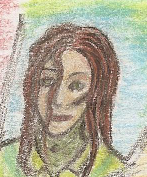
\includegraphics{sskreszta-portrait-alt-klein.png}\emph{Schimmernde
Farben wirbeln um den unscheinbaren, klaren Kristall. Dann breitet sich
ein sanftes Leuchten über seine Ecken aus, das sein Inneres erhellt, bis
er in sanftem weißen Licht leuchtet, in dem immer wieder farbige
Schlieren tanzen.}

\emph{Die Schlieren werden klarer, ein Gesicht scheint aus dem Kristall
heraus zu blicken. Geschlitzte goldgelbe Augen mit grünlichem Schimmer,
der auftaucht, wann immer sie sich bewegen. Sie blicken aus dem Gesicht
einer Menschenfrau. Eine lange Narbe zieht sich von ihrer Wange bis zum
Kinn und endet am Halsansatz, wo die Haut in feine grünliche Schuppen
übergeht, die sich unmerklich öffnen und schließen.}

\emph{Während das Gesicht deutlicher wird, überlagert es den Kristall,
wächst über seine Grenzen heraus und stabilisiert sich. Dann beginnt der
Mund Worte zu formen, die anfangs widerhallen wie Klänge aus der
Unendlichkeit und sich festigen, bis eine ruhige, klare Stimme aus dem
Kristall dringt.}

6000 Jahre sind vergangen, das sagt zumindest die Cryokapsel. Ob das das
Jahr als Göttin ausgleicht? So werde ich später kaum etwas mit den
Aufzeichnungen anfangen können. Versuch es zu strukturieren, Sskreszta,
auch wenn dir der Aufprall noch in den Knochen steckt. Nachdem Terrok
Nor zerstört wurde, habe ich Jodi Crown das letzte Mal gesehen. Er
sagte, die Station wäre schon das zweite Mal zerstört worden, und ich
glaube ihm, obwohl ich es nicht erklären kann.

\emph{° Eine Schlachtflotte schwebt vor der Station. Dann wird sie von
einem Lichtstahl erfasst und zerrissen.°}

Davor waren die anderen aus der Psionic 2, meiner ehemalige
Spezialeinheit, an Psionischen Angriffen gestorben, und ich sollte an
der Reihe sein. Jodi ist daraufhin einen Handel mit dem Wesen
eingegangen, das uns angegriffen hat: Er für mich. Dann verschwand
alles.

\emph{° Irisierende Augen beugen sich herunter, Lippen berühren sich,
alles wird grau.°}

\emph{° Weißer Dampf steigt auf und eine Plasttür öffnet sich nach
oben.°}

Als ich aufwachte, bin ich aus einer Cryokapsel gestiegen. Ihre Anzeige
sagte nur, dass 6000 Jahre vergangen waren.

\emph{° Eine nackte Frau steht mit aufgerissenen Augen vor einer Anzeige
neben der Plasttür. Ihr Körper ist vom Hals abwärts mit feinen Schuppen
bedeckt, die an den Seiten des Halses wie Kiemen auf und zu klappen. Im
nächsten Moment tritt ein Mann in stählerner Rüstung und einem
Langschwert in der Hand hinter sie. „Die ihr von den Sternen kommt, seht
mich an.`` Sie wendet sich um, sein Schwert entwindet sich ihm und
landet in ihrer Hand. Die Schuppen an ihrem Hals hören auf sich zu
bewegen.°}

Die Bewohner des Planeten haben mich als Göttin verehrt, bis ich von
einem Raumschiff gefunden wurde. Nach einer Weile wird es sehr
langweilig, wenn einem jeder Wunsch von den Lippen abgelesen wird. Kein
Wunder, dass Diktatoren dekadent werden. Hätte ich Kyrie nicht
kennengelernt, wäre ich wohl verrückt geworden.

\emph{° Vor einem Raumschiff verbeugt sich Sskreszta in Gewändern aus
fließender purpurner Seide vor einigen Berobten und Gerüsteten. „Ich
kehre nun zurück zu den Sternen. Denkt an meine Worte`` spricht sie,
bevor sie das Schiff betritt. Eine einsame Frau in Priesterroben blickt
ihr nach, als die Oberfläche des Planeten zurückweicht, immer kleiner
wird und zu einem Punkt in der Schwärze wird.°}

\emph{° Drei Raumjäger fliegen. plötzlich bricht einer aus und Streit
bricht über Kom los. Sie docken chaotisch an einem Transporter an, der
sie durch Sprungpunkte zu einer neuen Station bringt.°}

Ich bin den Rebellen beigetreten und Teil eines Psi-Geschwaders
geworden, das mir völlig unbekannte Taktiken verwandte.

Auf der neuen Station, einer Forschungsstation von gerade erst
entdeckten Aquatischen Intelligenten, hat sich vieles geändert. Von dort
an ging beinahe alles schief.

Stopp. Ich führe die Aufzeichnungen später fort. Wir haben einen alten
Bunker entdeckt, in dem wir hoffen Reparaturmaterial zu finden.

\section{Planetensturz}

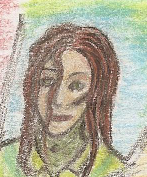
\includegraphics{sskreszta-portrait-alt-klein.png}\emph{° Blau
leuchtende Vögel mit einem Gefieder aus Blitz und Donner fahren auf
Sskreszta herab. Sie stößt sich von der Wand ab und zwei Schritte
vorwärts bringen sie an den Rand der Stahlplattform auf der sie steht,
während sie mit ihrer Linken eine elastische Plastikmaske über Gesicht
und Kopf zieht. Sie stößt sich ab und einen Augenblick später taucht sie
mit dem Kopf voran in ein Becken mit halbplastischer Flüssigkeit. Ein
Blick nach oben zeigt Blitze an der Oberfläche entlang zucken.°}

\emph{° Sie richtet eine Laserpistole auf ein riesiges schwarzes Auge in
einem deformieren Kopf. Der Kopf zuckt zurück und ein Laserstrahl brennt
sich in das Auge. Ein telekinetischer Angriff schmettert Sskreszta gegen
die Stahlwand.°}

Ich bin gerade aufgewacht, und hoffe jetzt noch die Zeit zu haben, meine
Aufzeichnungen weiter zu führen, während wir im Orbit um die zerstörte
Station auf die Scanergebnisse warten. Der gestrige Tag war anstrengend
und die Erinnerungen drängen sich auf. Ich führe sie nun wieder
chronologisch weiter.

\emph{° Ein Trägerschiff verlässt die Station. Es zerreißt in einer
Explosion. Sskreszta läuft in ihren Psijäger und schwebt zusammen mit
einem von einer Plane abgedeckten Stahlkonstrukt in den Frachtraum eines
Gleiters. Neben der Plane läuft eine Gestalt mit farbiger, feucht
glänzender Haut und Schwimmhäuten zwischen den Fingern, deren weißer
Forscherkittel ihre weiblichen Formen nicht vollständig verbirgt.°}

Ich bin nicht mehr Teil der Rebellen, seit wir die Station verlassen
haben.

\emph{° Sskreszta sitzt in dem Psiverstärker ihres Jägers.
Halbdurchsichtige Platten heben sich über ihre Arme und ein runder
Plasthelm senkt sich über ihren Kopf. Ihre Finger liegen sanft auf den
Tastenfeldern des Verstärkers. Sie zuckt kaum merklich, als ihre kleinen
und Zeigefinger gleichzeitig auf die Tastenfelder drücken.°}

Nachdem meine gesamte Einheit und mein Weg zurück zu den Rebellen
vernichtet waren, habe ich die Station in dem Gleiter eines Scouts
verlassen. Wir wurden auf dem Weg zum Sprungpunkt von mehreren Jägern
angegriffen.

\emph{° Um den Gleiter explodieren drei Jäger in schneller Folge. Dann
schweigen die Waffen des Gleiters und der Psijäger kehrt in den
Frachtraum zurück. Auf dem Kom des Psijägers erscheint ein Fuchsgesicht:
„Wir haben den Spungpunkt fast erreicht.``°}

Fox hat uns durch den Sprung gebracht. Dabei ist ein guter Teil der
Elektronik durchgebrannt. Direkt nach dem Sprung stürzten wir auf einen
Planeten. Weder mein Psischild noch die Flugfähigkeiten von Fox haben
ausgereicht um den Fall genug zu bremsen.

\emph{° Die Aquatische legt zwei durchscheinende Leitungsbahnen
zusammen. Ein helles Licht blitzt auf, dann legt sie ein schmales
Werkzeug zur Seite und die Leitungsbahnen glühen auf, als sie wieder von
Energie durchflossen werden.°}

Ich bin zusammen mit Fox auf die Suche nach Ersatzteilen für Kalem, die
Aquatische, gegangen, mit denen sie glaubte das Schiff reparieren zu
können.

\emph{° Auf einer Waldlichtung schälen sich Wände aus verwittertem Beton
aus dem Regen. Sskreszta und Fox zwängen sich durch ein halb aus den
Angeln gerissenes, verrostetes Tor. Sie sichern sofort den leeren
Innenraum, Sskreszta mit ihrem Blaster, Fox mit einem Schnellfeuergewehr
mit Schultergurt.°}

In dem unter der Lagerhalle liegenden Bunker haben wir etwa 20 Betten
gefunden, in denen 19 Tote lagen, deren Haut teilweise bis auf die
Knochen zerfressen war. Eins der Betten war leer und später fanden wir
in einer zerschossenen Konsole an der Wand eine Datenscheibe. Der
Computer im gegenüberliegenden Raum war seit 20 Jahren inaktiv gewesen.

\emph{° Sskreszta und Fox betrachten eine Gebäudekarte auf einem
Wandschirm. Sskreszta sagt bestimmt: „Zugriff auf die
Kameraaufzeichnungen``. „Zugriff nur für authorisiertes Personal``. „Wir
sind die einzigen Lebewesen in diesem Bunker``. „Falsche Information``.
Auf der Gebäudekarte blinkt im Kellergeschoss ein Lebenszeichen auf.°}

Durch eine Geheimtür kamen wir in den Forschungsraum des Bunkers. Ein
ehemaliger Arbeiter, der seit der Zerstörung des Bunkers dort lebte und
zu einem riesigen klumpen Fleisch mit Tentakelarmen und enormen
psionischen Kräften mutiert war, verlange von uns, ihn zurück zu
verwandeln, bevor er uns gehen lassen würde. Er schwebte auf einer
Plattform, an der er verschiedenste Waffen befestigt hatte. Am Ende
mussten wir ihn töten und er hätte mich mit seinen telekinetischen
Kräften fast zerschmettert. Wir haben dort mir bisher unbekannte
Technologien gefunden, die dem Transport des Projektes mittels
Teleportation dienten, an dem die Wissenschaftler dort forschten. Was
für ein Projekt das war, konnten wir nicht herausfinden, aber es muss
wichtig gewesen sein. Die Zielpunkte waren allerdings nicht verfügbar.
Anscheinend wurde die Teleportation in den 6000 Jahren, in denen ich im
Kälteschlaf lag, verbessert.\\ Zwischen den Diskussionen mit dem Wesen
konnte ich die oberen Bereiche des Bunkers noch einmal durchsuchen,
während es Fox unten gefangen hielt. Der Forschungsraum war mit einem
Energieschild gesichert, den ich nur durchbrechen konnte, indem ich
psionisch eine Geheimtür geöffnet habe. Davor habe ich meinen Blaster
bei dem Versuch verloren, die Tür von innen aufzuschießen.

\emph{° Ein Blaster schwebt vor einer glatten Wand. Ein Energiegeschoss
jagt aus dem Lauf gegen die Wand. Bevor es die Wand berührt, trifft es
auf eine Barriere, die es zurück auf den Blaster schleudert und ihn in
Stücke reißt. Die Explosion der Energiezelle zerstört einen Teil der
Wendeltreppe nach oben.°}

Das einzige unbesetzte Bett hatte einem Verräter gehört. In ihm fand ich
die Laserpistole, die ich am Ende auch gegen den Mutierten eingesetzt
habe. Während ich oben war, wurde das Gewitter stärker und der Mutant
verfluchte uns panisch, weil die Geheimtür nun offen war.

\emph{° Sskreszta klettert die halb zerstörte Wendeltreppe wieder
hinunter. Im Zentrum des riesigen Forschungsraumes liegt ein Becken mit
bleicher Flüssigkeit, das bis an den Rand des durch die Dunkelheit
eingeschränkten Sichtfeldes reicht. Ihre Schritte hallen von den Wänden
wieder und werden mehr und mehr von dem unregelmäßigen Zischen und
Bratzeln von Entladungen übertönt.°}

Die Basis wurde, wie den Daten des Computers nach schon zwanzig Jahre
vorher einmal, von vogelähnlichen Wesen angegriffen, die aus Blitzen zu
bestehen schienen. Glücklicherweise schützte die Flüssigkeit vor den
Entladungen, bis sie wieder verschwanden.

\emph{° Blau leuchtende Vögel mit einem Gefieder aus Blitz und Donner
fahren auf Sskreszta herab. Sie stößt sich von der Wand ab und zwei
Schritte vorwärts bringen sie an den Rand der Stahlplattform auf der sie
steht, während sie mit ihrer Linken eine elastische Plastikmaske über
Gesicht und Kopf zieht. Einen Augenblick später taucht sie mit dem Kopf
voran in ein Becken mit halbplastischer Flüssigkeit. Sie blickt nach
oben und sieht Blitze an der Oberfläche entlang zucken.°}

Fox gelang es, den Wesen außerhalb des Beckens zu entkommen, während der
Mutant sich wie ich unter Wasser sicherte. Als sie verschwunden waren,
tauchte er wieder auf. Ich versuchte Fox von einer Armwunde zu heilen,
schaffte es aber nur die Wunde oberflächlich zu schließen. Dann
verlangte das Wesen, dass ich auch es heile, obwohl Mutationen weit
außerhalb meiner Fähigkeiten liegen. Nach dem erfolglosen Versuch
richtete ich die Laserpistole auf sein Auge und befahl ihm still zu
halten. Es zuckte zurück.\\ Fox ist im Kampf trotz der primitiv
erscheinenden Technik seiner Waffe erstaunlich effektiv.\\ Wir haben in
den Resten seiner Panzerung und des Forschungsraumes zumindest die für
den Stellarantrieb nötigen Teile gefunden, nicht aber die für die
Sprungspulen.

\emph{° Sskreszta tritt aus dem Tor des Bunkers, das nun völlig aus den
Angeln gerissen ist, und überquert die kahle Erde auf der Lichtung um
das Gebäude, bis sie und Fox wieder im dichten Wald verschwinden.°}

\emph{° Die Frachtraumtür des Gleiters öffnet sich und Sskreszta und Fox
treten hinein, während immer wieder winzige statische Entladungen über
die Hülle des Schiffes zucken. Kurz darauf donnern die Triebwerke und
der Gleiter hebt auf einem Teppich aus blauweißem Feuer ab. Der Blick
auf den in der Entfernung immer kleiner werdenden Planeten offenbart ein
Wolkenband, das sich über dessen Oberfläche bewegt und in dem
unregelmäßig Blitze zucken.°}

\section{Stationsreste und Fundstücke}

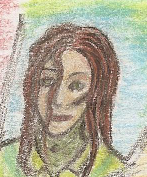
\includegraphics{sskreszta-portrait-alt-klein.png}\emph{°Ein
Vogelgesicht zeigt mit geschlossenen Augen zur Decke empor. Federn
rahmen ein Gesicht ein, in dessen Mitte ein kräftiger Schnabel glänzt.
Plötzlich öffnen sich die Augen und wache Intelligenz spricht aus
ihnen.°}

Wir haben Überlebende in der Station gefunden und ich glaube das Jahr
als Göttin hat meiner Selbstkontrolle geschadet. Von vorne:

Um einen anderen Planeten des Systems, dessen Struktur bereits so
instabil war, dass es jeder Zeit unerwartet zerbrechen konnte, kreiste
eine Station. Die Scans haben auf der Station kein Lebenszeichen und nur
Spuren elektromagnetischer Signale gefunden.

Ich bin mit Kalem zusammen im Jäger zur Station geflogen, um von der
Station zumindest noch verwertbare Teile zu bekommen, um damit den
Sprungantrieb zu reparieren. Statt ihrer unscheinbaren Technikerkleidung
hat sie vor dem Abflug eine silbern glänzende Kampfrüstung angezogen,
die zumindest zur Zeit der Raumflotte Zivilpersonen nur mit vielfacher
Genehmigung hätten besitzen, und dann auch noch lange nicht nutzen
dürfen.

Sie trug sie allerdings, als hätte sie darin bereits mehr als einen
Kampf überstanden. Als ich sie fragte, wie gut sie kämpfen könne, gab
sie keine sinnhaltige Antwort.

\emph{°Der Jäger verlässt das Schott des Gleiters und fliegt auf eine
Raumstation zu. Auf dem Schirm des Jägers erscheint das Gesicht von Fox:
‚Keine Lebenszeichen im Scan. Ich schicke euch die Pläne.
Energieversorgungen sind eingezeichnet.`°}

Wir landeten im Raumdock der Station. Kalem sprang aus meinem Jäger. In
der Hand hatte sie einen Stab, ähnlich einer Taschenlampe. Später erfuhr
ich, dass er ihre Waffe ist.

Die Schotts der Station waren beschädigt und wir hörten kreischende
Geräusche. In einem der Räume fanden wir eine Leiche, die vollständig
zerrissen war und in ihrer eigenen, erst vor kurzem getrockneten
Blutlache lag. In einem anderen Raum waren Leichen bis zur
Unkenntlichkeit verbrannt. Bei einem Toten war die Rüstung am Körper
festgeschmolzen. Lebenszeichen gab es auf der Station also keine mehr,
Leben aber sehr wohl.

\emph{°Sskreszta kniet sich neben einen mit einer halb-verschmorten
Rüstung bedeckten Körper. Sie greift die am wenigsten geschmolzene Kante
der Brustpanzerung und setzt den Fuß auf die Schulter des Toten.
Plötzlich knacken dessen Rippen, die Panzerung lockert sich ein Stück
und reißt mitsamt dem Brustkorb auf. Sskreszta zuckt zurück und drückt
dann den Brustpanzer wieder auf den Toten, während dunkles, zähflüssiges
Blut aus dessen aufgerissener Lunge quillt.°}

Unser Leben wäre allerdings fast nicht mehr darunter gewesen. In einem
Gang brachen die Sichtscheiben ins All, gerade als wir an ihnen
vorbeigingen. Das leise und immer lauter und häufiger werdende Knacken
von Panzerglas werde ich wohl lange nicht vergessen. Kalem konnte in
einen Raum mit funktionierendem Schott springen während mein
Pilotenanzug mich zwei Stunden lang hätte versorgen können.

Es gelang mir ein Kabel telekinetisch mit einer Stahlstange im nächsten
Schott zu befestigen und daran aus dem Gang zu kommen. Der Luftdruck
hatte sich auf etwa 10\% der Norm stabilisiert, während immer mehr Luft
aus der Station gerissen wurde. Kalem gelang es, sich die Luft anhaltend
bis zum Schott und auf die andere Seite zu ziehen. Ihre Spezies kann
unerwartet lange die Luft anhalten. Wie lange genau werde ich sie noch
fragen. Nachdem das Schott geschlossen war, stabilisierte sich der Druck
um uns wieder.

\emph{°Eine Metallstange blockiert ein halb geschlossenes Druckschott,
durch das Luft aus dem Gang gesogen wird. An einer weiteren Metallstange
hängt ein Stahlkabel. Das Kabel spannt sich. Kurz darauf packt eine Hand
in silbernem Panzerhandschuh die Schottwand und Kalem zieht sich durch
die Öffnung. Sie zieht scharf die Luft ein und bleibt schwer atmend
unter dem Schott liegen. Sskreszta zieht die Stahlstange aus dem Schott
und es schnappt zu.°}

Nachdem wir uns ein paar Momente lang erholen konnten, sahen wir uns in
einem weiteren Raum um, hatten aber kaum Zeit mehr als einen flüchtigen
Blick hinein zu werfen. Kaum waren wir aus dem Gang heraus, hörten wir
ein tiefes Brummen, das mir noch jetzt Schauer über die Schuppen tanzen
lässt.

Fünf Replikator-Spinnen kamen den Gang hinunter. An ihren vorderen
Gliedmaßen ließen sonische Klingen die Luft stark genug vibrieren, dass
sie den Hintergrund verzerrte.

\emph{°Sskreszta und Kalem zielen um den stählernen Türrahmen auf die
heranrückenden Spinnen. Bei jedem Schuss blitzen um die Spinnen
Schutzschilde auf. Plötzlich glänzt die Mundpartie einer der Spinnen und
eine Plasmaentladung schwärzt die Wand neben der Tür. Sskreszta: ‚Was
machen wir?`, Kalem: ‚Deckung` - Sskreszta: ‚Wir erwarten sie hier.`°}

Im nächsten Moment blitzte vor der Tür etwas grell auf und das Summen
stoppte. Ein Vogelmensch stand zwischen den Spinnen, eine ECM-Granate in
der Klaue, die ihre Systeme erneut lahmlegen konnte. Mangels
Alternativen folgten wir ihm und er führte uns in einen Raum, wo wir
seinen General treffen sollten.

\emph{°Für einen Moment füllt ein Vogelmensch den Türrahmen aus. Seine
Rüstung glänzt im Zwielicht des Raumes und sein Adlerschnabel richtet
sich auf Sskreszta und Kalem. Dann tritt er langsam und würdevoll vor.
In jeder seiner Bewegungen vibriert innere Kraft, jedes Zucken der
Klauen scheint bewusste Geste, jedes Blinzeln seiner Falkenaugen jagt
ein Beben durch Sskresztas Körper.°}

Ich kann weder beschreiben wie er in diesem Moment aussah', noch weiß
ich, was er gesagt hat, auch wenn ich mich an jede Nuance seines
Tonfalls erinnere.

Daher werde ich es nicht weiter versuchen. Er nennt sich Etaros. Mit ihm
bin ich durch ein Schott nach außen und wir sind über die Außenwand zu
meinem Jäger gekommen.

\emph{°Eine Luftschleuse öffnet sich. Mit einem Schwall Luft wird
Sskreszta aus der Station geblasen, in der Linken eine Rettungsleine,
die sie mit der Station verbindet, über die rechte Schulter ein
überschweres Blastergewehr. Ihre Augen weiten sich unter der
aufgeblasenen Schutzmembran ihres Anzugs als der Vogelmensch aus der
Luftschleuse schießt. Er trägt weder Helm noch Anzug und seine
ausgebreiteten Flügel tragen ihn durch den Raum als würden er auf winden
schweben. Nach kurzem Zögern zieht sich Sskreszta an der Rettungsleine
zur Station und klettert an den Haltegriffen über die Außenwand.°}

Endlich bei meinem Jäger angekommen, hörten wir erneut das Summen von
sonischen Klingen. Eine Replikatorspinne tauchte unter meinem Schiff
hervor und griff uns an. Bevor sie uns erreichte erschien in Etaros'
Hand ein kurzer Stab, an dessen Spitze eine Kugel glänzte. Die Kugel
blitze auf und die Spinne brach zusammen. Im selben Moment schwankte er
und brach zusammen. Während weitere Spinnen das Hangarschott
durchbrachen, sprang ich in meinen Jäger, loggte mich in den Verstärker
ein und levitierte Etaros in das Cockpit.

Über Funk erfuhr ich, dass Kalem und der andere Vogelmensch auf dem Weg
in die tiefsten Regionen der Stationen waren. Eine kurze Salve aus den
Jägergeschützen riss eine Bresche in die Station, durch die sie wie von
Fox vorhergesagt einen Moment später herausgeschleudert wurden. Ich zog
sie ins Schiff und stellte die Atmosphäre wieder her. Dann kehrten wir
zu Fox' Gleiter zurück. Die Ersatzteile für Fox Sprungantrieb hatten sie
im Lager der Station gefunden.

\emph{°Der zweite Vogelmensch trägt seinen General in eine der Kabinen.
Einige Minuten später tritt Sskreszta in die Kabine, kniet sich neben
ihn und legt ihre Hände auf seinen Brustkorb. Für einen Moment vibrieren
die Schuppen an ihrem Hals und öffnen und schließen sich in Wellen, doch
Etaros reagiert nicht.°}

Um ihm helfen zu können, haben wir ihn zu meinem Jäger gebracht. Ich
habe mich in den Psi-Verstärker eingeloggt und meinen Weg in seinen
Geist erzwungen. Er hat mir geantwortet und ich habe ihm daraufhin die
Kraft gegeben, die er brauchte, um wieder zu Bewusstsein zu kommen.
Obwohl ich den Psi-Verstärker hatte, hätte er mehr Kraft aufnehmen
können, als ich ihm geben konnte.

\emph{°Durchsichtige Plastplatten fahren aus den Armstützen über
Sskresztas Arme, dann senkt sich der Helm auf ihren Kopf. Vor ihrem
inneren Auge sieht sie Etaros' mentale Barrieren. Kurz tastet ihr Geist
an den Barrieren entlang, dann zwingt sie eine Bresche hinein und hört
seine Stimme.°}

Später testete Kalem, ob sie den Psi-Verstärker nutzen kann und konnte
sich fast komplett synchronisieren. Ich werde bald herausfinden, welche
Fähigkeiten sie sonst noch verbirgt. Wir werden ein schwieriges Gespräch
führen, und wenn ich ihr einen Blaster an den Schädel halten muss.
Hoffentlich gibt es bald den ruhigen Moment, den ich dafür brauche. Der
nächste Flug in dem wir zusammen in meinem Jäger sind, wird für sie
nicht der angenehmste werden.

Niemand widerspricht einer Pilotin, wenn sie in ihren Verstärker
eingeloggt ist. Zumindest nicht mehr als einmal.

Kalem installierte die Ersatzteile und wir werden springen können, bevor
der Planet, um den die Station kreiste, endgültig explodiert. Zumindest
wenn unsere Schätzungen stimmen. Ich hasse es auf ungenaue Schätzungen
angewiesen zu sein.

\section{Zivilisation?}

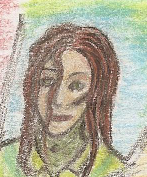
\includegraphics{sskreszta-portrait-alt-klein.png}\emph{„Wenn du
handelst, dann tu es bestimmt und ohne Zweifel. Besser eine läuft
selbstbewusst in den Abgrund, als alle versagen aus Zaghaftigkeit.``}\\
- Sskreszta

Wir sind wieder bei den Rebellen nachdem wir die Zivilisation erreicht
haben. Ich weiß nicht, ob ich mich wirklich darüber freue, doch ich
greife vor. Das wird mir wohl noch häufiger passieren.

Der nächste Sprung brachte uns in die Nähe eines bewohnten Planeten. Die
Bewohner bauen dort Gase und Minerale für Sprungantriebe ab.

\emph{°Langsam senkt sich der Gleiter auf die Planetenoberfläche. Aus
rot-grauer Wüste schälen sich Kreisformationen, von denen eine an Größe
zunimmt während die anderen hinter dem Horizont verschwinden. Eine
Mauer, gerade wie mit dem Laser gezogen, trennt sie von der offenen
Wüste und bietet Schutz gegen Sandstürme. Der Gleiter sinkt tiefer.}

\emph{7 Kuppeln sind nun zu erkennen, durch Polarisierung blau-bräunlich
schimmernd. Unter den Kuppeln stehen Häuser, eine ganze Stadt unter
durchsichtigem Plast und dahinter ein blassgrüner Fleck auf dem
Wüstensand.}

\emph{Mit donnernden Triebwerken senkt sich der Gleiter auf eine der
Kuppeln und taucht durch eine aufgleitende Öffnung ins Innere, in eine
andere Welt. Das gedämpfte Licht der Sonne scheint durch die Scheiben
bräunlich, alle Gebäude abgenutzt und gebraucht und auch der Gleiter mit
all seinen nun deutlich zu Tage tretenden kleineren und größeren
Beschädigungen fügt sich in das Bild.°}

Nach dem üblichen Empfang durch die Stationssicherheit, hat Kalem
angefangen, das Schiff wieder zu reparieren. Unser Hyperraumantrieb mag
zwar ein Flickenteppich sein, aber weitaus wichtiger sind doch die
Backupsysteme und zumindest rudimentäre Panzerung.

Als erstes lieferte sie eine Einkaufsliste. Sie war eindeutig eine
staatliche Forscherin, denn der Preis von Ersatzteilen scheint ihr
völlig unbekannt zu sein. Wir haben besorgt, was in unseren
Möglichkeiten lag, aber natürlich blieb mehr als die Hälfte der Liste im
laden zurück. Alleine die Kompensatoren hätten unsere Resourcen
überstiegen.

Der Verkäufer war ein Pflanzenwesen, klein, freundlich und er hatte
bereits mit Kalem geredet, so dass er genau wusste, dass wir die
Ersatzteile brauchte. Wenn sie so weitermacht, werden wir noch wirklich
zu Händlern.

\emph{°Ein Grinsen huscht über das Gesicht eines Wesens in staubiger
Wüstenkleidung, während ein kleiner Transporter Kiste über Kiste mit
Ersatzteilen auflädt. Auf dem Display auf der Innenseite des
Gleiterschotts rattert der Bordcomputer vor Sskresztas beinahe
schmerzverzerrtem Gesicht Preise herunter und der verfügbare Betrag
nimmt immer mehr ab. Dann öffnet sich das Schott und Sskreszta und Fox
beginnen mit dem Ausladen des Transporters.°}

Wir haben uns jedoch nicht sofort um die Einkaufsliste gekümmert. Die
erste Priorität nach der Landung auf dem Planeten liegt immernoch auf
der Ankunft. Wir mögen keine große Crew haben, aber das Essen für die
Reise ist seit jeher so wichtig, wie Reparaturen und aufzutanken. Ich
denke, Jodi Crown hätte das anders gesehen, aber die Zeiten ändern sich.

Während Kalem sich also wie üblich in Arbeit geworfen hat, habe ich mit
Fox den Raumhafen erkundet und nach seinen Spezialitäten durchsucht.
Nicht über alle von ihnen lohnt es sich wirklich zu sprechen.

\emph{°In der prallen Sonne liegt der längliche Kadaver eines Wesens, in
Scheiben geschnitten, rohes Fleisch, zwei Meter lang, einen Meter hoch
und breit, wie in Scheiben geschnittenes Brot. Der Händler grinst, nimmt
eine Scheibe des Fleisches, so breit und lang wie ein menschlicher
Brustkorb und vielleicht 5 Zentimeter dick, und reicht sie Sskreszta.
Sie weißt es mit beiden Händen zurück und beeilt sich weiter zu
kommen.°}

Später sollten wir auch noch auf die Lieferanten des Fleisches treffen.
HIKs, Halb Intelligente Kreaturen werden sie hier genannt, und sie gehen
sehr aggressiv gegen die hier lebenden Siedler vor, doch dazu später
mehr.

Nach dem ersten Versuch lokale Spezialitäten zu erwerben, entschlossen
wir uns für eine kleine Bar, die zum Glück auch nicht-Spezialitäten
servierte. es ist schde, dass Etaros nicht dabei war. Der Computer meint
übrigens, dass seine Spezies Malux genannt wird. Ob das stimmt habe ich
ihn noch nicht gefragt.

Wir hatten kaum gegessen, da taumelte ein Mann in grauer Robe durch die
Tür der Kneipe. Hinter ihm kamen einige Schläger. Ich weiß noch nicht
genau wieso, aber ich zog meine Laserwaffe, die ich bei der nächsten
Landung gegen den Ersatzblaster aus meinem Jäger austauschen werde. Eine
Laserwaffe gibt nicht das sichere Gefühl, das ein Blaster vermittelt.
Wenn der Blaster trifft, ist das Ziel mit Sicherheit ausgeschaltet. Eine
Laserwaffe kann abgelenkt, abgeschwächt, von schwacher Panzerung
abgehalten, reflektiert oder von kräftigen Wesen manchmal einfach
ignoriert werden.

Zumindest die Schläger schienen davon wenig zu wissen, und der gerettete
erwies sich als zahlender Passagier.

Wenn das alles wäre, das über ihn zu sagen ist, könnten wir sehr
glücklich sein, denn er bezahlte uns genug für die nächsten zehn
Sprünge. So wissen wir weder, wer er wirklich ist, noch was er will,
sondern nur, dass er hier angeblich 15 Jahre festsaß und gase abgebaut
hat. Außerdem hat er Probleme mit den Siedlern hier. Sie mögen ihn
angeblich nicht. Gründe nannte er keine. Wir trafen uns erneut bei den
Begründungsanlagen.

\emph{°Der Blick durch die Kuppelwand weist auf dunkleren Wüstenboden
aus dem an manchen Stellen Grasnarben ragen. Durch eine Öffnung in der
Kuppel treten Sskreszta in ihrem Pilotenanzug, die Schutzmembran über
den kopf gezogen, und Fox in einem Strahlenschutzanzug in die freie
Sonne. Vor ihnen erstreckt sich dunkler Wüstensand, gespickt mit grünen
Punkten, die sich mit wachsender Entfernung von der Kuppel vermehren und
eine geschlossene Rasenfläche unter den tödlichen Strahlen der Sonne
bilden. Weiter draußen säumen Bäume den Rasen und verschiedene Arten von
breitblättrigen Gräsern ragen aus dem Boden. Dort zwischen den Bäumen
steht eine einsame Gestalt in grauem Mantel anscheinend ungeschützt im
tödlichen Licht.°}

Er erzählte uns nicht allzu viel neues, doch alleine die Tatsache, dass
er ohne offensichtlichen Schutz im Licht der Sonne stand sagt viel über
ihn aus. Wir wissen nicht, welche Fähigkeiten er vor uns verbirgt, doch
unser dort geschlossener Handel besagt, dass wir ihn für eine Bezahlung,
die für die nächsten 10 Sprünge reicht, zum nächsten Planeten mitnehmen.

Zurück beim Raumhafen begannen wir mit den weiteren Einkäufen. Unsere
Bordküche hat seit diesem Tag statt einem Replikator eine Cryokapsel, in
der wir frisches essen lagern. Der Händler ließ sich überreden uns
Panzerplatten für unsere beschädigte Hülle kostenlos zu den Ersatzteilen
zu geben.

Die Qualität war entsprechend.

\emph{°An die Raumschiffwand gelehnt steht eine menschengroße
sechseckige silbergraue Panzerplatte. Plötzlich trifft ein Laserstrahl
auf die Platte. Wo er getroffen hat steigt leichter Rauch auf und die
Oberfläche der Platte zeigt eine unmerkliche Trübung. Sskreszta löst
ihren Handschuh und streicht mit dem Finger über die Stelle. Dann wendet
sie sich um.}

\emph{„Für mehr als Ablativpanzerung taugen die Platten nicht, Fox. Ein
Treffer und es reißt sie vom Rumpf. Einen Treffer auf die Triebwerke zu
stoppen ist aber besser als gleich zur Nova zu werden.``°}

Als wir in die Stadt zurückkehrten um noch w eitere Vorräte zu kaufen,
sahen wir, wie ein Teil der Mauer zur Wüste brach und sich
Insektenartige Kreaturen daraus in die Stadt ergossen. Ohne weiter zu
zögern traten wir ihnen entgegen, zusammen mit Kämpfern in massiven
Kampfrüstungen. wir erfuhren schmerzhaft, dass ihre Panzerung die Wesen
sehr effizient gegen Laserfeuer schützt. Fox' Projektilgewehr dagegen
verursachte massiven Schaden, so dass wir auch erfahren konnten, dass
das Blut dieser Wesen aus Säure besteht, die stark genug ist, um sich
durch schwere Panzerung zu fressen.

\emph{°Breitschultrig, die stählernen Füße fest in den Boden gestellt
und ein schweres Blastergewehr an der Seite jagt ein Kämpfer in schwerer
Panzerung Salve über Salve in die Gruppe der ankommenden Wesen.
Plötzlich bröckelt der Boden vor ihm. Mit rasender Geschwindigkeit löst
sich eine Mischung aus einem Käfer und einer Made aus dem Boden. Aus der
Kopfoberseite ragen Fühler mit Augen an den Spitzen und lange Klauen
zucken an beiden Seiten des Mundes, in dem kleine Beißwerkzeuge
unablässig arbeiteten. Es trifft frontal auf den Kämpfer und zerreißt
seine Rüstung. Ein letzter Schuss löst sich aus dessen Waffe und reißt
dem Wesen die Hinterseite auf. Es kriecht weiter vorwärts als Laser und
Projektilfeuer seine Panzerung trifft. Zwei Laserstrahlen verkohlen
seine Augenfühler, mehrere Projektile durchschlagen die Panzerung. Als
es stehen bleibt, treten Sskreszta und Fox zu den in der Säure
dampfenden Überresten des Kämpfers, dessen Rüstung sich von der
Brustplatte abwärts unter Säureblut langsam auflöst. Der Obere Teil
seiner Panzerung liegt mit den Überresten des Kämpfers zwei Meter
weiter, wohin das Wesen ihn mitgezogen hat, bevor es endgültig stehen
blieb.°}

Wir haben uns tiefer in die Stadt zurückgezogen. An einer Straßenbiegung
sahen wir Etaros, der immer wieder von einer unsichtbaren Kraft gegen
die Wand geschleudert wurde, aufstand und erneut zurückflog. Worauf er
feuerte sahen wir erst später. 20 Meter von ihm entfernt stand ein Wesen
aus Licht und Formen, dessen psionische Kraft alles überstieg, was ich
bis dahin gespürt habe, mit Ausnahme eines kompletten Gestalt aller
Mitglieder der Psi-Einheiten von Terrok Nor.

Als wir es konfrontierten, verbarg es seine physiche Gestalt, ich konnte
es jedoch noch immer psionisch wahrnehmen. Ein paarmal durchdrang mein
Laser seinen Psi-Schild, dann kamen weitere Angreifer dazu. Einer von
ihnen traf mich unglücklich in der Schulter. Zu meinem Glück kam Etaros
dazu und trug mich durch die Luft zu dem Schott zur Landungskuppel. Als
wir es öffneten spürten wir, wie eine psionische Präsenz hindurchglitt,
ich vermute die unseres Angreifers, denn das öffnen des Schotts öffnete
auch eine psionische Barriere.

Wieder bei unserem Schiff heilte mich Etaros mit seinen Kräften. Ich
vermute, damit ist unsre Rechnung beglichen, aber ich hoffe, er bleibt
trotzdem noch. Er hat mir ein Abendessen angeboten, das ich nicht
vorhabe auszuschlagen.

Nach zwei Sprüngen setzten wir unseren Passagier auf einem Planeten ab
und reisten mit den Sterndaten der Wüstenstation weiter um unsere Waren
abzugeben. Zum Glück stellte sich heraus, dass Kalem dort nicht bleiben
muss, denn sie ist eine extrem fähige Mechanikerin, auch wenn ihre
sozialen Fähigkeiten noch weniger ausgeprägt sind als selbst bei den
zurückgezogensten Kampfpiloten, die ich kennengelernt habe.

Bei der nächsten Möglichkeit hole ich aus ihr heraus, was sie wirklich
kann. Bisher hatten wir nicht die nötige Ruhe, und ich werde sie erst
konfrontieren, wenn sie die nötigsten Reparaturen beendet hat. Falls sie
vorhat uns zu verraten, sollte sie doch vorher unser Schiff in Ordnung
bringen, und falls sie sich für sich Sicherheiten installieren sollte,
werde ich die wenn nötig aus ihren Erinnerungen bekommen.

Fox dagegen weiß gut, wie man einen Landurlaub genießt, zumindest
nachdem er die nötigen Besorgungen für sein Schiff organisiert hat, und
seine Pilotenfähigkeiten lassen wenig zu wünschen übrig.

\section{Im Dienste der Rebellen (Kapitel)}

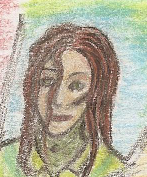
\includegraphics{sskreszta-portrait-alt-klein.png}\emph{Die Zeit,
die wir für die Rebellen als Organisation kämpften. Irgendwie war das
Leben da noch einfacher.}

\section{Piraten an den Versorgungslinien}

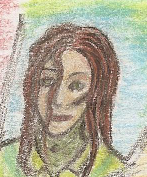
\includegraphics{sskreszta-portrait-alt-klein.png}``Widersprich
keiner Pilotin, wenn sie in ihrem Jäger sitzt. Es ist schmerzhaft und
sinnlos.'' - Sskreszta

Ich werde mehr als einen Eintrag brauchen, um die neusten Ereignisse
festzuhalten. Die letzten Tage ist viel passiert und mein Körper ist
sehr schwach. Ich bin noch am Leben, was kaum wahrscheinlich war, und
Etaros ist nirgendwo zu finden, und so zerbricht eine Entscheidung und
ich bleibe bei der Crew.

°Lichtblitze zucken im Cockpit, Stimmen verzerren sich, Echos hallen
immer lauter, übertönen jeden Klang, werden unerträglich. Die Helligkeit
der Blitze brennt in den Augenliedern. Die Form des Cockpits verzerrt
sich. Dann fällt das Schiff in den Normalraum zurück. Nach ein paar
Sekunden blinkt das Kom, der Navigationscomputer zeigt ein
Planetensystem und einen bewohnten Planeten als Ziel. Sskreszta nickt
Fox zu und steigt aus dem Copilotensitz. ``Ich mache einen Test des
Psiverstärkers mit Kalem.''°

Die Zeit, die wir zum Anflug brauchten, nutzte ich, um endlich die
Wahrheit über Kalem zu erfahren. Unter dem Vorwand, den Psiverstärker
während dem Flug überprüfen zu wollen, stieg ich mit ihr zusammen in
meinem Jäger auf. Sobald der Gleiter zu einem hellen Punkt im All
geworden war, sagte ich ihr, dass sie die Geräte wieder einpacken
sollte.

°Ein Kabel wird aus der eckigen Konsole des Verstärkers gezogen. Kalem
steht auf, ihre Haut wechselt rapide zwischen verschiedensten Farbtönen.
``Wer bist du wirklich?'', Sskresztas Stimme. ``Ich bin Kalem.'' - ``Wer
hat dich geschickt?'' - ``Ihr habt mich doch mitgenommen!'' - ``Wo hast
du so kämpfen gelernt?'' - ``Das ist ein Sport auf meinem Planeten. Ich
war nur eine mittelmäßige Kämpferin.'' Ein Blick Sskresztas hebt sie in
die Luft und schleudert sie an die Wand. ``Wo hast du so kämpfen
gelernt?'' - ``Das habe ich doch gesagt!'' Sie wird erneut gegen die
Wand geschleudert und von telekinetischen Händen festgehalten. ``Sag die
verdammte Wahrheit! Wer hat dich geschickt? Für wen arbeitest du
wirklich?'' - ``Niemand hat mich geschickt! Wie kommst du eigentlich
darauf? Ich sage die Wahrheit! Du kannst ja in meinen Geist schauen!''
Sie fällt zurück auf den Boden des Cockpits und ihre Gesichtszüge
verzerren sich vor Schmerz. Sie drückt die Schwimmhautbesetzten Hände an
den Kopf während ihre Gesichtsfarbe zu irisieren beginnt. Dann sinkt sie
gegen die Außenwand, die Augen vor Schmerz und Zorn funkelnd. Der Jäger
landet im Hangar des Gleiters. Kalem schwebt heraus. Dann tritt
Sskreszta aus dem Schott. Sie schließt das Schott des Jägers und sagt
``Es war ein Fehler.'' Dann geht sie zu den Kabinen.°

Kalem scheint es nicht sehr gut aufgenommen zu haben. Sie wird darüber
hinwegkommen. Zumindest weiß ich nun, dass sie die Wahrheit gesagt hat,
so wie sie sie sieht.

Der Stützpunkt, auf dem wir landeten, war offiziell in der Hand der
Union. Die Regierung war allerdings vollständig von Rebellen
unterlaufen. Auf ihm lag das Labor für Antriebstechnik, ein großes
Forschungszentrum der Rebellen und der Zielort für unsere Ware und auch
für Kalem. Sie sollte dem Auftrag nach zusammen mit dem Prototypen, den
sie entwickelt hatte, auf dem Planeten bleiben. Wir landeten und Fox
besorgte sich eine offizielle Lizenz für seine Waffe. Da weder Kalem
noch ich registriert sind, bleibt uns die Möglichkeit verwehrt. Leider
kann ich daher meinen Jäger nicht offiziell registrieren, so dass ich
ihn auf zivilisierten Welten im Gleiter lassen muss. Den Namen seines
Gleiters hat Fox uns noch nicht genannt. Für meinen Jäger werde ich
einen passenden Namen finden, jetzt da ich ihn noch länger haben werde.

°Ein Aufzug fährt rasend schnell in die Tiefe. Angekommen öffnen sich
die Türen zischend und Sskreszta tritt in einen weiten Gang mit einem
Boden aus milchigem Plast. Als sie vor eine Tür tritt öffnet sie sich.
``Kommen sie herein'', eine Stimme. Vor einem Tisch sitzt ein riesiger
Vogelmensch, ein Malux, fast so groß wie Etaros aber mit weitaus
breiteren Schultern, dahinter ein schmaler Mensch, ein Taschenkom in der
Hand.°

Wir wurden auf einen weiteren Auftrag geschickt. In der Nähe dieses
Stützpunktes bei einer Versorgungsstation der Rebellen gab es Probleme
mit Piraten. Wir entschlossen uns, den Anflug im Realraum zu machen. 4
Wochen Flugzeit. Hätten wir uns richtig vorbereitet, hätten wir später
weit weniger Probleme gehabt, doch es bringt nichts über Fehler zu
jammern.

Meine Konzentration nimmt ab, daher werde ich das Log zu einem späteren
Zeitpunkt fortführen.

\section{Piraten an den Versorgungsleitungen}

\emph{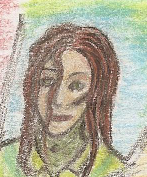
\includegraphics{sskreszta-portrait-alt-klein.png}°Mit
lautlosen Schritten schleicht Sskreszta an der Seite eines
Stahlcontainers entlang. Ihren Blaster auf Gesichtshöhe eines möglichen
Gegners haltend nähert sie sich der Ecke. Ihre Muskeln spannen sich und
ihr Zeigefinger zuckt unmerklich, während sie sich weiter voran schiebt.
Dann katapultieren ihre Beine sie nach vorne, der Blaster zuckt zur
Seite, ihr Blick tanzt um die Ecke und ein Lächeln umspielt ihre Lippen,
als sie Fox mit gesenkter Waffe erblickt. Im nächsten Moment wirft ein
Ruck an ihrem Bein sie zu Boden, aus dem Stoff ihrer Uniformhose reißen
blauen Fetzen und der gesamte Kistenstapel setzt sich in Bewegung.
Einige Zeit später kippt Fox die letzten Kisten von Sskreszta herunter.
Nach ein paar schweren Atemzügen erhebt sich Sskreszta, lässt ihren
Psi-Schild fallen und beginnt zu fluchen.°}

Wir sind auf dem Rückweg von unserem Auftrag, und ich weiß noch nicht
genau, was mit mir passiert ist, aber ich bin sicher, etwas von dem
Wesen, das mich dort abgegriffen hat, ist noch immer in mir. Ich werde
es herausfinden, doch jetzt, da ich dringend eine Pause von unserem
Training brauche, muss dieses Log endlich fertig werden. Es ist schon zu
lange unvollständig, und meine Erinnerungen verlieren bereits an
Schärfe.

Die 4 Wochen, die unser Hinflug dauern sollte, verbrachte ich
hauptsächlich mit meinem Training und in der Kantine. Auf dem Planeten
hatten wir uns mit echtem Essen ausgestattet und es in zwei zusätzlichen
Kryokapseln gelagert. Es macht einen enormen Unterschied, ob man morgens
Rationen der Raumflotte oder fast frisches Obst und Brote vorfindet.

\emph{°Die Kryokapsel schließt sich zischend. Im selben Moment öffnet
sich lautlos die Tür zur Kantine und die Silhouette Etaros' erscheint im
Rahmen, breit und würdevoll wie ein Sternenkrieger aus Flottenmythen.
Langsam tritt er auf die Kryokapsel zu, sein Vogelgesicht erhoben, die
Augen wach und klar und auf Sskreszta gerichtet. Wie erstarrt bleibt sie
stehen, während er sich ihr nähert. Als er nur noch zwei Schritte
entfernt ist, nickt sie ihm zu und wendet sich abrupt dem Erhitzer zu.
Ihre Hände beginnen zu zittern, als sie die Finger von dem verschweißten
Reispaket löst und ihre Handfläche auf den Startknopf des Erhitzers
presst.°}

Auf der Station wurden wir von einigen Tech begrüßt, die es von Anfang
an geschafft haben uns zu nerven. Dass sie uns mit einer Feier begrüßen
wollten, war noch akzeptabel, weniger aber, dass sie unter einer Feier
verstanden, die ganze Zeit lang laut über Nutzloses zu reden. Immerhin
hatte Fox alte Gravball-Spiele in den Schiffsdatenbanken, so dass sie
meistens beschäftigt waren. Die Probleme begannen Recht bald, so dass
wir zum Glück auch beschäftigt wurden. Ich erinnere mich nicht mehr an
alles, seit mir der Wandler sein Gift injizierte, aber ich zeichne das
auf, was ich noch weiß.

\emph{°Eine dünne Nadel berührt Sskresztas Hals. Als sie die Schuppen
durchdringt, schießen Schmerzen durch ihren Körper. Während sie in die
Knie bricht, sieht sie Fox über den Boden auf sie zu schlittern, seine
Waffe im Anschlag.°}

Der erste Angriff kam, als die Techs dort endlich vom Feiern müde waren
und wir noch einmal an der Kantine vorbeigingen.

Weitere Geschehnisse:

\begin{itemize}
\item
  Arbeiter: Sidan (Energiewesen), Enjes (Leiter), Ines (Synarchu, Freund
  stirbt).
\item
  In der Kantine Angriff durch unsichtbare Gegner. Fox hat sie entdeckt,
  indem er mit dem HUD und den Schiffssensoren die Gaskonzentration im
  Raum überwacht hat: Ausatmen, Methankonzentration.
\item
  Kalem hat mit den Arbeitern gesprochen. Noch zerstreuter als sie,
  mindestens genauso in ihre Arbeit vertieft, auf Schwebeplattform im
  Bauhangar.
\item
  Wir haben ein Schott in den hinteren Teil der Station geöffnet, der
  von fast totalem Vakuum erfüllt war.
\item
  Kalem hat die Gänge hinter dem versiegelten Schott durchsucht.
\item
  Sskreszta hat Klauenspuren in der Station gefunden, als wäre etwas
  sehr starkes durch die Gänge nach außen geschleift worden und hätte
  die Klauen tief ins Metall der Gänge geschlagen. Selbst auf der
  Außenwand der Station noch einige Spuren, bis es wohl durch das All
  davon gezogen wurde.
\item
  Weiter hinten war ein Transporter angedockt, in dem wir ein schwarzes
  Wesen gefunden haben, das uns angriff. Wir Immobilisierten es
  (Granate). Jack schnitt es mit dem Laserschwert auf. Erst schien es,
  als würde die Klinge eingesaugt, dann brach das Wesen auf und zwei
  Lichter stiegen aus ihm in die Höhe. Sie flogen ins Cockpit, wo Etaros
  lag, und schlüpften in seinen Körper. Er blieb unbewegt und wir
  brachten ihn raus und in unseren Gleiter. Fox versiegelte den Gleiter.
\item
  Kalem wurde, nachdem sie alleine weiter nach Nützlichem gesucht hatte
  (um Waffen bauen zu können), in ehemaligen Arbeiterquartieren in den
  Vakuumgängen, von unbekannten Gegnern angegriffen, die nur ein
  Sauerstoffmundstück trugen. Die Gänge scheinen nicht so leer zu sein,
  wie die Stationsarbeiter hier behaupten.
\item
  Sie hat sich Stück für Stück ins Dock zurückgezogen. Dann hat sie den
  Kopf eines toten Gegners als Ablenkung über die Schottwand gehoben,
  der sofort von Schüssen zerschmettert wurde und zerplatzte. Dann
  schloss sich das Schott, während wir versuchten, das Schott auf der
  anderen Seite zu öffnen.
\item
  Wir trafen uns wieder in der Kantine. Die Arbeiter waren guter Dinge.
  Sie meinten, wir hätten die Feinde komplett besiegt, und jetzt wäre ja
  wieder alles gut. Dann wollten sie feiern. glücklicherweise ging da
  der Alarm los.
\item
  Am Schott gab es wieder Probleme. Kalem und Jack waren als erste da
  und metzelten einige Piraten und einen Kämpfer in leichter
  Kampfpanzerung nieder.
\item
  Der Kämpfer in Kampfpanzerung wurde von Jack immobilisiert, dann
  warnte ihn Kalem, aufzuhören sich zu wehren und hielt ihm ihre
  sonische Klinge gegen das Visier. Als er nicht aufhörte, färbte sich
  ihre gesamte Haut schwarz, die Augen glühten rot, und sie ließ ihre
  sonische Klinge ausfahren.
\item
  Kurz darauf wurden wir in den Gängen der Station erneut angegriffen.
  Einige Piraten hatten ein schweres Gauss-Gewehr, sie hatten fast alle
  leichte persönliche Schutzschilde. Einer davon ist jetzt in Sskresztas
  Quartier.
\item
  Dann wurde Kalem von einer Kopie ihrer selbst angegriffen. Ihr Gegner
  war ihr in Verhalten und Aussehen fast völlig gleich. Sskreszta hat
  den falschen entlarvt, indem sie Kalems Waffe und eine sonische Klinge
  zwischen die beiden warf. Natürlich war Kalem an ihrer Waffe, während
  ihr Gegner in perfekter imitation dessen, wie sie am
  wahrscheinlichsten hätte reagieren müssen, nachdem sie den Gepanzerten
  abgeschlachtet hatte, vor dem sonischen Schwert zurückschreckte. Wir
  schossen auf ihn, und als er in der Ecke lag ging Sskreszta auf ihn
  zu.
\item
  Sie hielt ihm die waffen an den Kopf und kam langsam näher. Im
  nächsten Moment schoss sein Arm vor, riss ihr in unerwarteter
  Geschwindigkeit die Waffe aus der Hand und packte sie als Geisel. Er
  zog sich mit Sskreszta im Schwitzkasten langsam zurück, während die
  anderen folgten.
\item
  Aus dem Arm des Gegners kam eine dünne Nadel und ritzte Sskreszta am
  Hals. Sie wurde zum ersten Mal seit Jahren von Schrecken übermannt und
  bettelte um ihr Leben.
\item
  Plötzlich rannte Fox auf die beiden zu. Die Nadel stach in ihren Hals
  und Sskreszta Gliedmaßen wurden schlaff. Dann wich ihr Gegner zurück,
  Fox schlitterte über den Boden an ihm vorbei und schoss ihm in den
  Rücken.
\item
  Sskreszta kam wieder zu sich und wir deponierten den Leichnam des
  Wandlers in einer geschlossenen Kabine.
\item
  Sskresztas Zustand verschlechterte sich plötzlich. Gliederschmerzen,
  Kopfschmerzen, Schwindel. Sie lief auf den Hangar mit dem Gleiter zu,
  stolperte, kroch weiter, rief über Funk um Hilfe.
\item
  Kalem sprang in Sskresztas Jäger, loggte sich in den Psiverstärker ein
  (ist kompatibel, frühere Versuche schon), und lenkte es ungelenk aus
  dem Gleiter. Sie schrabbte über den Boden und kam zu Sskreszta, ludt
  sie ein und holte sie ins Schiff. Dort heilte Kalem Sskreszta.
  Sskreszta hatte vor und während der Heilung Visionen (Ein
  Höhlensystem, das sie durchwandert, Markierungen, die sie auf den
  Boden setzt, um sich zurechtzufidnen) und danach das Gefühl, dass
  etwas von dem Gift ihres Feindes zurückgeblieben ist.
\item
  Kalem und Jack gingen erneut in die Station, während Fox' Gleiter sich
  nähernde Schiffe meldete. Fox kümmerte sich um mehrere Gleiter,
  während Sskreszta (immernoch völlig fertig) mit dem Jäger um die
  Station flog und dort zwei kleine Gleiter zerstörte (nachdem ein
  Raketentreffer ihre Schiffslaser abgesprengt hatte, wich sie den
  nächsten Raketen aus, flog zum Cockpit ihres Gegners und versuchte ihn
  telepathisch zu übernehmen. Dann bemerkte sie, dass die Rakten ihr
  gefolgt waren und kam gerade noch weg, bevor sie in das gegnerische
  Schiff einschlugen). Einen Transporter, der am hinteren Teil der
  Station angedockt hatte, machte sie flugunfähig (Triebwerke psionisch
  zerrissen).
\item
  Vorne wurd Fox von einem getarnten Jäger angegriffen. Sskreszta nahm
  ihn psionisch war, hängte ihren Jäger an das Schiff und sagte Fox
  ``schieß unter mich''.
\item
  Wieder auf der Station zeigte sich, dass der Gleiter sabotiert worden
  war. Löcher in eer Außenwand, verschlossen durch kleine
  Schildgeneratoren. Im Energiesystem des Gleiters gibt es seitdem eine
  hartnäckige Energiespitze, die auch durch massive Reparaturen nicht
  entfernt werden konnte. Kalem und Sskreszta fanden die
  Schildgeneratoren bei einem Testd er Außenhülle (drei Generatoren, die
  zusammen zwischen sich einen Schild aufbauen). .
\item
  Wir sammelten den Schiffs-Schrott ein, den die zerstörten Gegner
  hinterlassen hatten.
\item
  Mit Etaros in der Cryokapsel flogen wir zurück.
\item
  Training auf dem Rückflug, Patzer von Sskreszta, 4 5-er, bleibt beim
  Sprung um einen Kistenstapel an ihm hängen und er stürzt auf sie
  herunter.
\item
  brachten Etaros in schwerem Kasten zurück (Schutz und Abschirmung),
  Spec-Ops holten ihn ab.
\item
  Kalem in die Klinik wegen mentaler Narbe. War danach völlig fertig,
  weil sie den mentalen Schaden wieder erhielt.
\item
  Alle ließen sich mental heilen.
\item
  Sskreszta stand an Etaros' Bett, nahm ihn mit raus. Dann verschwand er
  wieder wegen seinen Geschäften. Die Info, dass er wieder draußen ist
  kam, nachdem er schon wieder unterwegs war.
\end{itemize}
\section{Ein besonderes Etablissement}

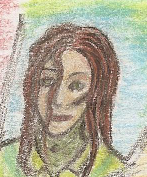
\includegraphics{sskreszta-portrait-alt-klein.png}Wir sind in ein
Bordell gegangen, in dem wir Spaß suchten (Der andere Vogel (nicht
Etaros) hatte uns Zugang verschafft, vermutlich mit unehrlichen
Methoden). Dort war ein ``Berger'', wir stoppen Leute, die mit ihren
Rüstungen in Arenakämpfe wollten, ``Dämpfen'' stoppte die Rüstungen,
Frost ließ sie sterben.

\emph{(Der andere Vogel war Jack, gespielt von einem Spieler, der nur 2x
dabei war)}

Dann kämpften wir gegen Onyx, die Feuerbälle schleudern könnten und Fox
und Kalem flohen durch eine Seitentür.

Ich wurde von Gestalten in Kutten in eine Traumrealität gezogen, in der
ich durch einen Gang wanderte, in dem Messergras wuchs.

\emph{(Die Ausflüge in die Traumrealität sind ein Aspekt der Kampagne,
der mir immer sehr viel Spaß gemacht hat!)}

Ich kam bei Fox und Kalem wieder aus dieser Traumrealität, in einer
Kampfbasis mit illegalen Laboren.

Wir töteten Wachen und Kampfhunde mit Laserpistolen mit bleibendem
Strahl, starben fast in Gasfallen und fanden ``Ani'', eine
Wissenschaftlerin, die raus wollte (zumindest nachdem ihr klar wurde,
dass ihr sowieso Kollaboration vorgeworfen werden würde).

\emph{(Außerdem: Gefängniszellen, vor denen die Wachen waren)}

\begin{center}\rule{3in}{0.4pt}\end{center}

\emph{Dieser Eintrag war etwas kürzer, wie es auch einige der nun
folgenden sein werden. Es sind Aufschriebe aus den Anfangszeiten unserer
Kampagne, die die Geschichte auf dieser Seite vervollständigen. Ich
hoffe, sie bringen euch auch in diesem Format Lesespaß!}

\section{Licht am Ende des Tunnels}

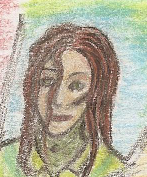
\includegraphics{sskreszta-portrait-alt-klein.png}Geschehnisse
nach dem Kampf im ``Etablissement'' und dem finden der Basis dahinter.

\begin{quote}
\emph{Geschichte, Stichworte, noch 7 mal, dann wieder Prosa}

\end{quote}
\begin{itemize}
\item
  Unterirdische Basis.
\item
  Weg gewechselt =\textgreater{} Ani gefragt, wo es lang geht, Weg war
  ``verschmutzt'' (Gift, nur Kalem konnte rein, weil mein Anzug bereits
  aufgebraucht war, hat die Luft angehalten), Ani Nervenzusammenbruch
  \begin{itemize}
  \item
    Stim für Ani \#Punkt für Sskreszta?
  \end{itemize}
\item
  Weiterer Weg. Ani bricht zusammen, blickt auf die Kamera, seltsame
  Überaktivität =\textgreater{} Blutdruck =\textgreater{} Ohrfeige von
  Sskreszta
\item
  Auf Liege in ausgeräumter krankenstation geröncht und gecheckt

  \begin{itemize}
  \item
    Chip entdeckt, durchs ganze Gehirn
  \item
    Ich schon zu fertig. Kalem versucht es, nachdem ich sie frage,
    gelingt die Verbindung zum Rückenmark zu trennen. \#Neue Handlung
    für Kalem. Punkt?
  \item
    Sskreszta gestützt von Fox, Erschöpfung.
  \end{itemize}
\item
  Ani getragen. Weiterer Weg =\textgreater{} Zwei Kampfbestien
  erschossen (Kalem).
\item
  Lifte. Sind über die Lifte nach unten, Jack fast zu schwer. Hilft beim
  herunterkommen auf den lift. Kann Computer auf Entfernung hacken.

  \begin{itemize}
  \item
    Ich springe ihm nicht in ie Arme \#Punkt für Sskreszta?
  \item
    Auf's Dach
  \end{itemize}
\item
  Bahnsteig.

  \begin{itemize}
  \item
    Monorail
  \item
    Roh behauen. Von Links Wind =\textgreater{} Nach links (Fox, Wasser
    - Tropfen fließt). \#Punkt für Fox?
  \item
    Bin unterwegs zusammengebrochen. Fox trug mich.
  \item
    Mit Gleiter zurück.
  \item
    Gleiter in die Stadt geschickt.
  \end{itemize}
\item
  Beim Schiff zurück. Ani (Wissenschaftlerin) in Cryokapsel.

  \begin{itemize}
  \item
    Nächster Tag. Ani abgeschirmt. Zu Antriebsforschung = Rebellen
  \item
    Kalem bekommt ihn rein, mit ungenauen Andeutungen. Nehmen meine
    Drohung nicht ernst.
  \item
    Wachen kommen raus, agrressiv (zur Seite stoßen) Störsender.
  \item
    vorher längeres gespräch mit Fox. Spezies, Familienverhalten, viel
    offenbart. Hat erzählt, was bei Ranmex ausgestoßen bedeutet. Für
    Familie auch.
  \end{itemize}
\item
  Habe mich Heilen lassen

  \begin{itemize}
  \item
    Seelendoc unfähig. Erst beim zweiten Versuch fähig.
  \item
    Psi-Runde mit Kalem.
  \end{itemize}
\item
  Bericht geschrieben.
\item
  Kitains rief uns

  \begin{itemize}
  \item
    Etaros, Krankenbesuch.
  \item
    Angeblich Virus (klar\ldots{} Streitgespräch, Arzt hat uns natürlich
    nichts gesagt)
  \end{itemize}
\item
  Kalem wurde getestet !Nicht erzählt

  \begin{itemize}
  \item
    ``Natürlich habe ich gute Reflexe. Ich werde ja ständig von
    irgendwelchen leuten mit Gegenständen beworfen, da muss ich
    ausweichen können.'' -Kalem \#Punkt!
  \item
    ``Betrogen, wegen cheatens des testers verloren.''
  \item
    Gegangen. Am nächsten Tag gekündigt (eingereicht).
  \item
    Hat sich in ihrem Zimmer eingeschlossen\ldots{} \emph{grr}
  \end{itemize}
\item
  Etaros kommt wieder raus.

  \begin{itemize}
  \item
    Erzählt.
  \item
    Kalem geht wohin auch immer.
  \end{itemize}
\end{itemize}
\section{Schatten im Tunnel}

\begin{figure}[htbp]
\centering
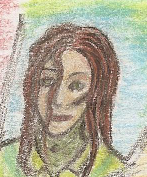
\includegraphics{sskreszta-portrait-alt-klein.png}
\caption{Sskreszta, altes Bild}
\end{figure}

\begin{quote}
\emph{Geschichte, Stichworte, noch 6 mal, dann wieder Prosa}

\end{quote}
\begin{itemize}
\item
  Gespräch im Schiff "Kalem kündigung, musste raus, Planung Rest)
\item
  Kalem zu Antriebstechnik, Wegen bestätigung von kündigung. Nicht
\item
  Nicht gekündigt, general degradiert, dafüentschuldigung an Kalem
\item
  Kalem zurück zum Schiff, Sskreszta fragt Kalem
\item
  In die Kneipe wegen ``Para'' finden (Ranmex, infiziert von Symbionten)
\item
  Kneipe

  \begin{itemize}
  \item
    Onyx-Türsteheer mögen Kalem und Jack nicht. Erst nach 400cr zahlung
    reingelassen (``machen Probleme'')
  \item
    Waffen abgeben
  \item
    Sskreszta saß am Tisch mit Logan
  \item
    Fox mit Ranmex gesprochen, ``Logan'' infos
  \item
    Andere spielen
  \item
    Sskreszat und Logan Spielen
  \item
    Kalem spielt vor den anderen, spielt nicht mit den anderen
  \item
    gemeinsamer Kampf im Spiel Logan, Sskreszta, Fox, Jack
  \item
    Anheuerung von Logan (2000cr für mitkommen)
  \end{itemize}
\item
  Nächster Tag: Treffen und Höhle

  \begin{itemize}
  \item
    Materialeinkauf
  \item
    Höhle unter Sand
  \item
    Etwas bewegte sich im Sand (Sskreszta Wahrnehmung aus Jäger)
  \item
    In den Tunnel hinunter
  \item
    Signal- und Lichtblocker (Statikfeld)
  \item
    Mit Seilwinde herunter, Kalem levitiert sich
  \item
    Flak unterm Sand beschießt Gleiter
  \item
    Sskresta hört es, als sie kurz raus geht
  \item
    Fox hoch, Kontakt mit Schiff, Rückzug + Gegenangriff
  \end{itemize}
\item
  Höhle

  \begin{itemize}
  \item
    An der Tür, gespräch mit paranoidem ``Para''
  \item
    Logan überzeugt ihn, dass wir rein durften
  \item
    Sskreszta und Logan rein, überzeugten ihn, dass die anderen rein
    durften
  \item
    Alle mit Waffen außer Jack, nur mit Rüstung, aber ohne Gauss
  \item
    Para sah sehr mitgenommen aus, teilweise verbrannt, manchmal grüne
    Augen
  \item
    ``Verhandlung''
  \item
    ``Para'' mit Symbionten, weibliches Wesen in ihm, er konnte es
    verdrängen
  \item
    Er hinter sehr dicker Glasscheibe
  \item
    Bei Erwähnung von Kalem als Psionikern, Raum abgedunkelt und Scheibe
    geschwärzt
  \item
    Später wieder hell, aber Scheibe blieb dunkel
  \item
    para mehrfach in ZWeifel gebracht wegen Vertrauen zum Symbionten
  \item
    Para hat erzählt, dass das Imperium die Rebellion kontrolliert
  \item
    Die unteren Eben wirklich gegen System,
  \item
    Obere Ebenen gehorchen dem System
  \item
    Psi nur eine Illusion: Krankheit, Viren die durch Licht übertragen
    werden, Von Xynoc geschaffen
  \item
    Para stimmte zu, mitzukommen, wenn er eine 5-er Leibwache mit
    Kortexbomben, 5 Panzer und 2 Jäger als Leibwache
    (\emph{tock.tock.tock})
  \item
    Zwei mussten drin bleiben
  \item
    Unsere Wahl.
  \item
    Kalem und Jack freiwillig (\emph{eg})
  \item
    Fox gibt Jack EMP-Granate (\#Teilpunkt für Fox)
  \item
    Sskreszta, Logan und Fox zusammen zu Rebellion
  \end{itemize}
\item
  Sskrszta, Logan, Fox in der Stadt (zur Rebellion)

  \begin{itemize}
  \item
    Logan durfte nicht rein, Zigarette geraucht
  \item
    Sskreszta, Fox, Anfrage wegen Eskorte (=\textgreater{} Eskorte von 2
    mit falschen Kortexbomben)
  \item
    Planung, Ideen: Magnesiumfackeln zum blenden (\#Teilpunkt für Fox),
    Seismischer Bohrer, Bomben in den Schacht werfen\ldots{}
  \item
    Fox: Hintereingang: Unterirdische Bahn (\#Teilpunkt für Fox)
  \item
    Einkaufen: Viel. Fox hat Top-Ausrüstung gekauft (Klettern, Luft,
    Seilwinde, 1t Zug, Selbstreplizierendes Seil, etc.)
  \item
    Auf den Weg zu Schienenbahn
  \end{itemize}
\item
  Kalem, Jack in der Höhle

  \begin{itemize}
  \item
    Langeweile für jack, Kalem zeichnet und fachsimpelt mit Para,
    bekommt Tipps für Antrieb
  \item
    Kalem wollte was praktisches machen, Para sagte, Kalem könnte St. 17
    Schild basteln, sollte aber erst Stufe 3 Schild probieren, wurde St.
    4.
  \item
    Angriff
  \item
    Wackeln,
  \item
    Rumpeln,
  \item
    Angriff von Säurebestie,
  \item
    Augenschuss von Kalem
  \item
    Weiterer Angriff
  \item
    Schießen beide, treffen Psi-Jäger (Gerade nicht durch Psi-Schild und
    Panzerung)
  \item
    Sskreszta Rückzug, V-Laser (illegal!) schießt, zerschießt
    Steingeschoss von sskreszta
  \item
    Biowesen kommen durch den Gang hinter dem Jäger (Bioelektrisches
    Feld kündikte sie an).
  \item
    Kalem und jack überreden para kurz Waffen auszuschalten,
  \item
    Sskreszta kommt vor, greift nicht nach Geist von para
  \item
    waffen wieder aktiv
  \item
    Jack hackt Tür
  \item
    Kalem in die Tür, Jack fliegt wieder raus
  \item
    Kalem belabert Para (\#Punkt für Kalem)
  \item
    EMP-Granate von Jack schaltet Elektronik aus
  \item
    Zugriff von sskreszta auf Paras Gehirn, block
  \item
    Kalem hotshotted Jacks Waffe
  \item
    Biowesen kommen an Jäger heran
  \item
    Werfe sie ineinander
  \item
    immer mehr, werden zu viele
  \item
    Sskreszta lässt die Decke einstürzen, Gang blockiert
  \item
    Vision, Jack, Kalem, Sskrezta: Gang Vision sskreszta: Gang, Tür,
    Dunkelheit, hineingetreten, von Hand in die Höhe gezogen, ins Licht
    =\textgreater{} Höhle mit Ei, Weiter weg: Insel, weiter weg: Planet,
    weiter weg: Von Planet weg (später wieder erkannt)
  \item
    Biowesen kommen wieder durch
  \item
    Jack schießt am Jäger vorbei
  \item
    Druckwelle, Jäger in Gang geworfen, Wesen tot, Jäger verschüttet,
    Psi schild fällt aus
  \item
    Kalem zu Para: Kuttenwesen (Mit Skelletthand)
  \item
    Wesen streckte Skellethand aus zu Para, Hand wurde grün, wurde
    fleischfarben, Überzog sich mit Haut, Wesen verschwand.
  \item
    Sskreszta wacht wieder auf, wieder Vision
  \item
    Versuche auf karte die Insel zu lokalisieren, gefunden Alle in
    Sicherheit
  \item
    Fox legt zweiten Zugang (Mittlere Laser verdampfen Stein, graben)
  \item
    Sskreszta: Freigesprengt (Telekinese)
  \item
    Plünderung :-)
  \item
    Gaus-Waffe von Jack zerstört
  \end{itemize}
\item
  Para zurückgebracht, Bezahlung erhalten
\item
  Logan angeheuert (500cr + Urlaub auf Tropeninsel)
\item
  Auf zu neuen Ufern
\end{itemize}
\emph{2 Punkte für Fox, 1 zus. Punkt für Kalem, 1 zus. Punkt Logan}

\section{Flammende Frosttunnel}

\begin{figure}[htbp]
\centering
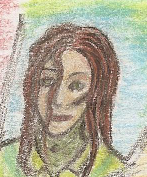
\includegraphics{sskreszta-portrait-alt-klein.png}
\caption{Sskreszta, altes Bild}
\end{figure}

\begin{quote}
\emph{Geschichte, Stichworte, noch 5 mal, dann wieder Prosa}

\end{quote}
\subsection{Rückkehr von dem Institut für Antriebstechnik}

\begin{itemize}
\item
  7,5kcr Belohnung erhalten, aller außer Kalem
\item
  Habe nach Infos für die insel gesucht
\item
  Geologisches Institut
\item
  Topologische Daten
\item
  =\textgreater{} Auftrag für die Daten: untersuchungen (Liste mit
  Tieren\ldots{})
\end{itemize}
\subsection{Reparaturen: 3 Wochen für Jäger}

\begin{itemize}
\item
  Sskreszta und Fox: Stadtbesichtigungen, Verschiedene Fotos
  geschossen\ldots{}
\item
  Kalem meistens unauffindbar
\end{itemize}
\subsection{Vorbereitung auf die Expedition}

\begin{itemize}
\item
  2 * Tropenausrüstungen (für 10kcr)
\item
  Macheten
\item
  Für Kalem: Nur Medkit für 3kcr)
\end{itemize}
\subsection{Flug zur Insel}

\subsection{Landungstest}

\begin{itemize}
\item
  300m über Boden kein Nebel mehr
\item
  200m über Boden kein Statikfeld mehr
\item
  Es sind Luftblitze, Statische Ungleichgewichte in der Luft
  (Ladungsverschiebungen)
\item
  bis 5m über Boden
\item
  Tiefenscan
\end{itemize}
\subsection{Demonstration von Schutzschild}

\begin{itemize}
\item
  persönliches von Kalem: Versuch Blaster gegen Schädel Kalems zu
  schlagen
\item
  Ins Schiff eingebaut
\item
  Test: mit kleinen Lasern auf Jäger geschossen. Schild hält 2 bis 3
  Laserschüsse aus.
\item
  Test Elektronik: Laserpistole an Seilwinde runtergelassen
\item
  Kalem: "Seilwinde nicht auf Schiffswand sondern auf Schrott: Material
  wird genutzt für Seil\ldots{} \#1 Punkt für kalem
\item
  2 Blitzeinschläge an Seil.
\item
  Laserpistole explodiert beim Einschalten durch Sskreszta (ESP\ldots{}
  kein Personenschaden)
\item
  mögl. durch Blitzeinschläge
\end{itemize}
\subsection{Höhlenscan am Berg}

\begin{itemize}
\item
  auf 3 mögl. eingegrenzt
\item
  An Seil runter
\item
  2 Fehlversuche =\textgreater{} Magnesiumfackeln kaufen geflogen,
  Rückkehr
  \begin{itemize}
  \item
    erste Höhle: Mit Jäger rein, Magmablase
  \item
    zweite Höhle:
  \item
    Fox erschoss Schlange durch Eis
  \item
    Sskreszta:
  \item
    Schlange gespürt (ESP):
  \item
    Plötzlich selbst raus, Schlange springt, erschossen
  \end{itemize}
\end{itemize}
\subsection{Dritte Höhle}

\begin{itemize}
\item
  3 Stunden am Seil durch die Höhle gewandert\ldots{} Langeweile\ldots{}
\item
  Einige Abzweigungen, nur aus Hauptweg Luftzug
\item
  In verschiedeneste Richtungen gegangen, immer dem Hauptgang nach
\end{itemize}
\subsection{Eisfläche}

\begin{itemize}
\item
  Statik
\item
  Statik hört auf
\item
  Sskreszta versucht Eis zu schmelzen

  \begin{itemize}
  \item
    ``Du willst Feuer?''
  \item
    Magmastrom aus dem Eis
  \item
    Angriff durch PsiWesen, sehr schnell
  \item
    Sskreszta weggeschleudert, Fox an Seil hinterhergerissen
  \item
    Mit Psischild über den Boden geflogen, stopp
  \item
    Kalem von Seil übers Eis geschleudert (pers. Schild)
  \item
    Gegen Wand geflogen
  \item
    In Loch eingebrochen
  \item
    3 Schlangen winden sich um Kalem (um Schild)
  \item
    \emph{pfrz} Schlangenköpfe gegrillt
  \item
    Sskreszta: aufgerichtet, Fox noch da, Kalem verschwunden.
  \item
    Wesen greift Sskreszta an der Schulter
  \item
    Schleudert S. übers Eis, Fox löst Seil
  \item
    Sskreszta richtet sich auf, weggerissen von Wesen (am Hals)
  \item
    Wesen Zerrissen von Schuss, Psischild im selben Moment gebrochen,
    Blitzerscheinung bei Wesen, verschwunden
  \item
    Kalem: ``War levitiert, hat Wesen erschossen.''
  \item
    Statisches Rauschen taucht wieder auf
  \item
    Wieder zusammengekommen
  \end{itemize}
\item
  Rast\ldots{} Sskreszta in Kokon, Kalem in Tropenzelt (warm), Fox
  Wache\ldots{}
\item
  Fox weckt Kalem: Statik verschwunden. Kalem Wache. \emph{--CUT--}
\end{itemize}
\section{Eisbrüche und Wassersuche}

\begin{figure}[htbp]
\centering
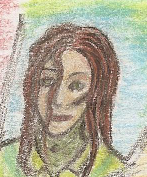
\includegraphics{sskreszta-portrait-alt-klein.png}
\caption{Sskreszta, altes Bild}
\end{figure}

\begin{quote}
\emph{Geschichte, Prosa, noch 4 mal, dann wieder Prosa}

\end{quote}
Gletscher bricht =\textgreater{} Fall in Gletscherspalte, Schlangen,
Gemeinsam am Seil hängen, Fox und Sskreszta \ldots{}\\ \ldots{}\\ Suche
in den Tunneln, Vision Sskreszta (Fall ins Wasser, weggetragen)
\ldots{}\\ \ldots{} Suche in Flüssen \ldots{}\\ \ldots{}\\ Graben im See

\emph{-cut-}

\section{Hö(h/l)lenspiele}

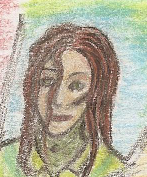
\includegraphics{sskreszta-portrait-alt-klein.png}\emph{Heute
nochmal außer der Reihe Notizen aus dem Gedächtniskristall. Warum außer
der Reihe? Schaut doch mal auf Datum und
Zeit\textsuperscript{\href{http://1w6.org/print/book/export/html/59\#fn:datum}{1}}.
Das konnte ich nicht verpassen! :)}

\begin{quote}
\emph{Geschichte, Stichworte, noch 3 mal, dann wieder Prosa}

\end{quote}
\begin{itemize}
\item
  Teile das Wasser (Sskreszta)

  \begin{itemize}
  \item
    Fox schießt durch das geteilte Wasser und zerbröselt den Boden
    =\textgreater{} Sehen Finden Gang, wie gegraben.
  \item
    Wir sind abgetaucht, kurz in den Gang geguckt, dann aufgetaucht
    (frustriert)
  \end{itemize}
\item
  Explosion am Wald (Nameless (Ghost, Nica) hatte schon die Zat gesehen,
  war unsichtbar geworden, Mine gelegt, geflohen)

  \begin{itemize}
  \item
    Fox und Kalem zum Schiff (Hangar), Sskreszta in den Kampf gg Zat
  \item
    Fox greift mit ein, Zat springen auf Gleiter, Fox: ``Guck, dass du'n
    Gurt findest'', Kalem: ``Zum festhalten'', Fox: ``Nein, zum
    Festschnallen!''
  \item
    Fox mit Gleiter, Kopfunterflug durch Baumwipfel, viel Spaß, Zat :)
    \#Punkt für Fox
  \end{itemize}
\item
  Sskreszta fliegt über Nameless, die unsichtbar schwimmt

  \begin{itemize}
  \item
    Zat springt auf Jäger, Psi-Angriff führt zu Splosch =\textgreater{}
    Säureblut
  \item
    Schnelles einladen von Nameless (sie wird im Jäger sichtbar),
    Tauchgang und Wirbel im Wasser (Sskresztas patentiertes
    Turbo-Waschgang-Manöver). \# Punkt?
  \end{itemize}
\item
  Fox watet durch Zat (Blaster gegen Zat\ldots{} )
\item
  Jäger zurück in den Hangar
\item
  Nameless steigt aus, Waffe in Hand

  \begin{itemize}
  \item
    Kalem in Hangar, Fox auch
  \item
    Sskreszta tritt von hinten aus dem Gleiter dazu: ``Bitte leg Waffe
    ab'', ``Wenn er es auch macht'' (zu Fox), ``Legt die Waffen ab'',
    ``OK''
  \item
    Verhör (Unsichtbarkeitsanzug (angeblich war es der Anzug),
    Personalien gesehen, angeblich Schiffbrüchige, wollte in Stadt,
    Agentin der Regierung in Finanzangelegenheiten, Auftrag in der
    Stadt, Chip mit dem Auftrag, Taxi in der Stadt genommen).
  \end{itemize}
\item
  In der Stadt Tauchausrüstung gekauft (aus 5000 pro Ausrüstung
  (Händler, Internet: 2000) wurden 4000 für alle). Dichtungsbeutel für
  Waffen gratis dazu (Fox).
\item
  Zum See, in den See getaucht

  \begin{itemize}
  \item
    Kalem nochmal hoch, Seil geholt. Kalem levitiert, schwimmt, in ihrem
    Element.
  \item
    Strömung wurde immer stärker, immer tiefer rein. Entscheidung einen
    Gang nach oben zu nehmen.
  \item
    Es gab viele Gänge, aus denen Wasser schoss, haben einen gefunden,
    aus dem es nur Plätscherte
  \item
    Kalem levitiert hoch, Fox und Sskreszta kämpfen sich hoch
    (irgendwann lev Sskreszta Fox, dann zieht er sie hinterher).
  \item
    Kalem zieht Seil ganz hoch, windet es um Stalagmiten. Fox und
    Sskreszta ziehen sich hoch.
  \item
    Kalem tritt in Schleim. Arne: ``Nein, ein Blob!'', Kalem: ``Zats''.
  \item
    Am Ende des Ganges größerer Blob (Schleimblase), blockiert den
    Wasserweg. Wir entscheiden se nicht zu zerstören\ldots{}
  \item
    Zatling taucht auf, Sskreszta schießt, levitiert ihn.
  \item
    Fox findet Blob, der die Wand imitiert, Wird weggebrannt. Sskreszta
    tötet Zatling (3 Schuss).
  \item
    Gang hoch, gestoppt, gerade bevor wir in einen großen Raum kamen
    (Abgrund)
  \item
    Kalem levitiert runter, an Seil, von Zat angegriffen
  \item
    Fox erschießt Zat
  \item
    Fußschritte hinter Sskreszta, dreht sich um, Stups\ldots{} langsamer
    Sturz rückwärts von Vorsprung \# SL-Punkt?
  \item
    Fox springt ein Stück zurück, wird geschlagen, Sturz
  \item
    Fox und Sskreszta, Sturz ins Wasser,
  \item
    Im Wasser schwammen Eier, Fäulnisgeruch, riesige Halle.
  \item
    Kalem und Sskreszta spüren Kälte. Eine Stimme ``Kommt zu mir''.
  \item
    Kalem versucht beide zu halten (mit Seil). Erste Panikprobe: Fox und
    Kalem panisch (Fox: Wunde von Zatschlag im Wasser dreckig,
    entzündet\ldots{} Kalem: Panisches am Seil ziehen um irgendwen zu
    retten, durch Psibelastung, Psischub).
  \item
    Sskreszta hakt sich aus, Fox auch, als die Panik bei ihm nachlässt.
  \item
    Finden uns durch Lichtsignale. Kalem zieht Sskreszta zum Rand
  \item
    Fox von Kalem gefunden, hakt sich ans Seil, vor rausziehen packt ihn
    etwas, erst ein Tentakel, dann etwas anderes (für Sskresztas
    Psikraft fühlte es sich wie eine große Hand an), Kalem zieht am
    Seil, Sskreszta zieht mit Psikraft.
  \item
    Sskresta bekommt Stein an den Kopf, KO.
  \item
    Kalem versucht Seil um Stalagmit zu binden, Stalag bricht, beim
    versuch um 2. zu binden Überlastung, Ohnmacht.
  \item
    Fox heruntergezogen,
  \end{itemize}
\item
  Aufwachen im Wasserbecken mit Wasserfall. Völlig klares Wasser, Steg
  außenrum.

  \begin{itemize}
  \item
    Ein Ausweg, folgen Steg aus der Höhle.
  \item
    ``Hatschi! Verdammter Schnupfen!'' - Mädchenstimme \# Punkt SL
  \item
    Fox riecht bekannten Geruch aus der Vergangenheit, Familie.
  \item
    Vorsichtiges hinterherschleichen. Leerer gang, Sskreszta wird
    plötzlich von Tatzen in Nische gezogen.
  \item
    Kalem tritt in den Gang, Mädchen aus dieser Nische schießt auf
    Kalem, keine Reaktion (Halber Schild verloren).
  \item
    Tatze auf Sskresztas Mund, als sie die Waffe auf Handgelenk richtet,
    ziehen die Krallen Blut, zweite Kralle auf Bauch. Waffe auf Mädchen
    gerichtet. Nimmt plötzlich die Waffe ab, springt, Psionisch gefangen
    (``Lass mich os, oder ich breche ihr auf sechszig Arten das
    Genick'').
  \item
    Kalem: Schuss auf die Decke zum Einbrechen (Grund: Moralische
    Bedenken, Hemmungen).
  \item
    Staub wallt auf, Tatze schlägt Sskreszta in den Nacken, stolpert
    raus, Griff verloren.
  \item
    Kalem feuert in die Nische\ldots{} Nische futsch.
  \item
    Sskreszta mit Psi-Sinn durch Staub gegangen, kein Mädchen/Tatzen.
  \item
    Kalem heilt Sskresztas Genick + Kratzer.
  \end{itemize}
\end{itemize}
\emph{Fox immer wieder Wahrnehmung, Punkt?}

\begin{itemize}
\item
  Engpass im Gang, Fox sieht von hinten zwei Minen. \# Fox Punkt?
\item
  Kalem und Sskreszta zurück. Sskreszta mit ganzer Psikraft und 1min
  Konzentration Minen mit höchster Geschwindigkeit weggeschleudert.
  Winzige Explosionen\ldots{} (Puff).
\item
  Dahinter Gang mit Sand. Formation (für Rest des Abends): Kalem vorne,
  Sskreszta in der Mitte, Fox hinten).
\item
  Kalem levitiert über Sand, Sskreszta tippelt an die Wand gedrückt um
  den Raum herum, Fox begutachtet Sand =\textgreater{} Sand = Asche.
\item
  Raum mit Säule. Rechter Gang (Gänge mit Brandspuren abgetrennt).
\item
  Fox überprüft Luft, Teil Links der Höhle feuchter und wärmer.
\item
  Links wahrscheinlich Geysir (heiße Quelle), doppelt abgetrennt.
\item
  Rechts zweimal durchstochenes Herz (erstes zentriert, fast vor linkem
  Gang), zweites vor einer Kuhle mit einer Pfütze (darüber auch ein
  Kreis eingebrannt).
\item
  Sand überprüft, seltsam trocken trotz Wasser. Wasser seltsam klar und
  dickflüssig.
\item
  Sand rausgeschaufelt. Unten wurde der Sand blutrot.
\item
  Sskreszta packt hinein, in Asche, die unten ist und sich weigert
  rauszukommen. undeutliche Visionen, Schmerzverzerrtes Gesicht, blass,
  nichtmenschlich. Beginnt zu schreien, fast im Schmerz verloren.
  Zurücktaumeln.
\item
  Wollten Raus. Plötzlich sieht Fox den Sand wieder reinfließen. Sand
  bildete eine Säule, dann eine Figur. Beginn zu schreien. raus. Bei
  übertritt der Linie endet das Schreien.
\item
  Mittelgang: Sackgasse.
\item
  Gang links: Niedriger Gang (Kindergang).
\item
  Durch, Wände wie Lebender Schleim. ESP sagt, einen Meter dahinter war
  Wand.
\item
  Hinten war eine Blase. Sskrestza berührt Blase, klopft Psionisch an.
  Kräftiger Gegenschlag.
\item
  Fox Kalem spüren Boden vibrieren, Sskreszta spürt, dass sich in Blase
  etwas tut, Fox spürt unter Boden etwas herauskommen.
\item
  Zatlinge und Hydralisken tauchen auf. Sskreszta aktiviert Psi-Schild.
\item
  4 Zatlinge greifen Kalem an, geht unter zweien zu Boden, dabei einer
  erschossen, Stab fährt aus.
\item
  Zwei Zatlinge greifen Fox an, einer erwischt ihn an der Schulter.
\item
  Hydralisk spuckt Sskreszta an, verfehlt.
\end{itemize}
Kampf:

\begin{itemize}
\item
  Reaktion: Sskreeszta 22, Fox, Kalem, 20, Zat 21.

  \begin{itemize}
  \item
    Sskreszta hält Hydralisk Blaster vors Maul und drückt ab. Hydralisk
    tot. \# Punkt Sskreszta?
  \item
    Zat: Zwei auf ihr liegende greifen Kalem an. Einer rutscht an
    Rüstung ab, anderer frisst Stabseite.
  \item
    Zat: Zatling greift Kalem von hintern an: Stabtreffer.
  \item
    Zat: Zatling gelingt es nicht Fox zu beißen, Fox gelingt es weniger
    schlecht zurückzuschlagen und er erschießt Zatling. Zweiter ebenso
    erschossen.
  \item
    Zat: 2 Zatlinge greifen Sskreszta an, einer verfehlt, zweiter trifft
    Psi-Schild, rutsch ab.
  \item
    Kalem: Erschießt Zatling und schießt auf Hydralisken =\textgreater{}
    H. brüllt.
  \item
    Fox: Tötet Zat, schwingt sich hoch (Boden) und schlägt Machete in
    die Wand um außer Reichweite zu sein. \# Punkt?
  \end{itemize}
\item
  Runde 2:

  \begin{itemize}
  \item
    Kalem: Verfehlt einen Hyralisken, auf zweiten: Kopfschuss.
  \item
    Hydralisk spuckt Säure auf Fox.
  \item
    Kampf zwischen Kalem und Zatlingen. erster Zat, Stabsitze, 2. Zat,
    anderes Stabende, Stab zu schwer\ldots{}
  \item
    Fox löst Anzug mit Knopfdruck, jetzt in Pilotenanzug. Einhändiger
    Kopfschuss Hydralisk.
  \item
    Sskreszta legt Zat--Hive Hand auf, Mental: ``Hör auf, du
    verlierst''.
  \item
    Zwei Zatlinge greifen Kalem an, schwingt sich über Stab und trifft
    sie zu Boden. \# Punkt Kalem?
  \end{itemize}
\item
  Runde 3:

  \begin{itemize}
  \item
    Sskreszta von zwei Zatlingen von hinten angegriffen. Bemerkt es
    gerade noch, dreht sich um. Ist schneller.
  \item
    Erster erschossen, zweitem den Blaster vorgehalten und grinsend
    nicht abgedrückt. Du kommst eh' nicht an. \# Fox, Kalem, Sskreszta
    Punkt?
  \item
    Zatling packt Fox am Bein.
  \item
    Fox tritt nach Zat, Zat weg. Fox zieht die Machete aus der Wand,
    lässt sich fallen, zieht im Fall die Waffen von der Schulter, legt
    mit beiden Händen an und erschießt den Zatling vor Sskrezta.
  \item
    Augenblick später durchpeitsche Schuss von kalem die nun leere Luft
    vor Sskreszta.
  \end{itemize}
\item
  Sskreszta legt Hand auf Zat-Hive. ``Gib auf, du verlierst''.
\item
  Zwei Zatlinge rennen vorbei (Fox hat bereits die Schutgun raus und
  damit zwei Waffen). Vier Schüsse aus vier Waffne erlegen zwei
  Zatlinge.
\item
  Quietschen von Hinten. Nochmal. Ultralisk kommt. Versuchen uns
  schießend zurückzuziehen, Fox beginnt Rucksackinhalte einzusammeln.
  (Auf noch zwei kl. Energiezellen und eine mittlerer Energiezelle
  darin).
\item
  Kalem Wirft volle Energiezelle und schießt darauf. Sskreszta schon am
  rauslaufen, dann sieht sie Fox, dreht sich um und wirft sich über ihn,
  Psi-Schild überladend. \# Punkt Kalem schon bekommen
\item
  Energiezelle explodiert. Nuklearexplosion?
\item
  Aufwachen, nicht fühlen, sehen, hören. Sicht kommt langsam zurück. Fox
  schwer verletzt, aus dem Bein ein Teil herausgerissen. Kalem schwer
  verletzt, beide Arme gebrochen, unbenutzbar, Rüstung gebrochen.
  Sskreszta schwer verletzt, tiefer Bauchschnitt. \emph{Anmerkung:
  Panikprobe, Kalem versaut sie.}
\item
  Sskreszta kriecht zu Medkit. Kalem versucht aufstehen, Fehler,
  Ohnmacht.
\item
  Sskreszta bekommt Medkit aktiv (Halb override). Erst Schmerzmittel und
  Stim dann Bauch halb geflickt.
\item
  Sskreszta heilt Fox, der gekommen ist.
\item
  Sskreszta drück Kalem auf den Boden, Heilt sie.
\item
  Sskreszta bricht zusammen. \# Punkt Sskreszta?
\item
  Kalem bricht vor Panik erneut zusammen.
\end{itemize}
\emph{Die Runde hatte lange Nachwirkungen, auf allen Ebenen.}

\begin{center}\rule{3in}{0.4pt}\end{center}

\begin{enumerate}
\item
  \texttt{2012-04-23 23:42:30}
  \href{http://1w6.org/print/book/export/html/59\#fnref:datum}{up}
\end{enumerate}
\section{Eiersuche-Wasserfall}

\begin{figure}[htbp]
\centering
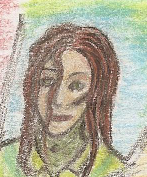
\includegraphics{sskreszta-portrait-alt-klein.png}
\caption{Sskreszta, altes Bild}
\end{figure}

\begin{quote}
\emph{Geschichte, Stichworte, noch 2 mal, dann wieder Prosa}

\end{quote}
\begin{itemize}
\item
  Nach Versorgung (med) zum Wasser
  \begin{itemize}
  \item
    Auf dem Weg ein Nieser gehört
  \item
    Sskreszta Ohnmächtig bis Wasser (von Kalem geweckt)
  \item
    Traumerinnerung (``Geistesblitz'')
  \end{itemize}
\item
  gegenüber der Nische, in der vorher die Mädchen und Ranmex standen,
  War Platte auf dem Boden (nach Graben von Kalem)
\item
  Kalem drück 4 Mal, 4 Zeichen leuchten (Feuer, Wasser, Licht/Energie, +
  4 andere zusammen)

  \begin{itemize}
  \item
    Barriere bricht ein, Sskreskat räumt es weg (erschöpfend).
  \item
    Licht kam aus dem anderen Ende des Ganges =\textgreater{} Sehen
    paradiesische Lichtung
  \item
    Barriere im Weg.
  \end{itemize}
\item
  Nach Graben auf dem Boden weitere Zeichnung (vier Pyramiden) von Kalem
  gefunden.

  \begin{itemize}
  \item
    Langes probieren (elemente nutzen schnell gefunden, aber dann lange
    kaum was geklappt)
  \item
    Ergab Hologramm in der Luft, bei Berührung wurde es invertiert.
  \end{itemize}
\item
  Fox schließt den Eingang zum Gang mit Platte innen (Felsen flogen
  zurück, er sprang noch durch).
\item
  Fox findet erstes Ei bei auseinanderfliegenden Steinen. Insgesamt
  finden wir 4 und Asche.

  \begin{itemize}
  \item
    Sowohl Ei als auch Asche waren halbmateriell/(halbreal
  \end{itemize}
\item
  Eier auf die 4 pyramiden (waren die Zeichen drauf)
\item
  Asche auf Eier =\textgreater{} Eier Platzen auf, zeichen drin (siehe
  Zeichnung)
\item
  Beide Arten von zeichen hintereinander auf die Pyramide, verschwanden
  jeweils bei wechsel.
\item
  Wesen aus Licht erscheint. Sagt etwas (s. Notizen)
\item
  Durch Paradies gewandert, Fußballfeldgroß, Wald

  \begin{itemize}
  \item
    See darin, darin Eier.
  \item
    Gingen an der Luft kaputt (in Sekunden) =\textgreater{} Kurzer
    Lichtschimmer/Lichtblitz
  \item
    Selber Lichtblitz beim zerscshlagen.
  \item
    Kalem am Wasserfall hoch. Gang in den Felsen, Zergwürmer im Wasser
    =\textgreater{} Kalem lebt, Zerg tot.
  \item
    Luftschoicht wurde zu schmal, Strömung zu stark =\textgreater{}
    Rückkehr.
  \end{itemize}
\item
  Gefäße für die Eier gebastelt, jeder eins.
\item
  Mit Seil in den Wasserfall.
\item
  Im Wasserfall:

  \begin{itemize}
  \item
    Sskresta stößt gegen Kalem, von kalem trotz heftigster Gegenwehr
    beatmet.
  \item
    Fox hat Atemmaske
  \item
    Sskreszta verliert ei. Kalem verliert Ei (Mehrere Stöße in die
    Rippen?)
  \item
    nur noch Fox' Ei
  \end{itemize}
\item
  An der Oberfläche. Im Meer unter Klippen

  \begin{itemize}
  \item
    An den Klippen hoch (Kalem levitiert, Rest hängt sich dran.)
  \item
    Oben ruft Fox den Gleiter =\textgreater{} Ei in Kryokapsel
    =\textgreater{} Rückkehr, schnell zurück (Sskresztas verschiedenste
    Stimpacks und Schmerzhemmer versagen langsam.
  \end{itemize}
\item
  Schwer überhöhte Geschwindigkeit über dem Stadtgebiet.
\item
  Polizei verfolgt uns ``landen sie'', Fox meldet Krankentransport,
  Polizei ignoriert
\item
  Landung vor Krankenhaus, Polizei kommt rein.

  \begin{itemize}
  \item
    Kalem mit Sskreszta raus. Sskreszta droht mit Psi, agiert. Kalem
    argumentiert (Sskreszta braucht Stütze)
  \item
    Sskreszta auf Bank vor Klinikum.
  \end{itemize}
\item
  Schwarze Limousine fährt vor.

  \begin{itemize}
  \item
    Generalin Jane steigt aus (die nicht bekannt ist).
  \item
    Sskreszta richtet Laser auf sie, warnt sie ``bleib stehen''. Arm
    wird lahm.
  \item
    Jane geht in den Gleiter.
  \item
    Kalem folgt ihr.
  \end{itemize}
\end{itemize}
Kalem: ``Als ich den Gleiter betreten wollte, konnten es sich diese zwei
Idiontischen Polizisten einfachnicht verkneifen, mich zu nerven. Da sie
mich nicht durchlassen wollten, warnte ich sie vor:''Lasst mich durch,
oder ihr spürt die Konsequenzen!``. Da sie nicht auf mich hören wollten,
legte ich sie flach und ging schnurstracks in das Schiff Ich beeilte
mich der Generalin zu folgen und bemühte mich dabei, nicht gesehen zu
werden. Während ich dem Gespräch zwischen der Generalin und Fox
lauschte, kamen von hinten schon wieder zwei Polizisten auf mich zu und
meinten, ich sollte doch bitte mit ihnen gehen und das Schiff verlassen.
Ich machte ihnen klar, dass ich von der Besatzung bin, doch sie wollten
nicht auf mich hören. Als ich ihnen sagte, sie sollten doch auf eigene
Gefahr versuchen, mich vom Schiff zu schaffen, versuchten sie doch
tatsächlich mich anzugreifen. Nachdem sich herausgestellt hatte, dass
die generalin Fox befreite und das rechtliche Regelte und damit mein
Verweilen auf dem Schiff gerechtfertigt war, schaute ich mitleidsvoll in
dei gesichter der armen, auf dem Boden liegenden Polizisten und meinte
nur:''Tut mir echt leid Jungs, ich hatte euch gewarnt``, und ging meines
Weges; zurück zu Sskreszta.''

\begin{itemize}
\item
  Jane aus dem Schiff. Sskreszta richtet Waffe auf sie und fragt über
  Funk bei Fox nach. Als das gespräch beendet ist,, fährt die Limousine
  gerade ab.
\item
  Sskreszta in Krankenhaus (wird reingeholt) =\textgreater{} 4 tage
  Aufenthalt. Rebellen übernehmen alles.
\end{itemize}
\section{Kampf den Göttern (Kapitel)}

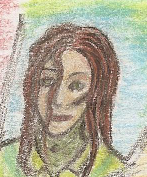
\includegraphics{sskreszta-portrait-alt-klein.png}\emph{Wir
stellen uns gegen die
\href{http://1w6.org/deutsch/welten/raumzeit/spezies\#xynoc}{Xynoc}
{[}7{]} selbst, um
\href{http://1w6.org/deutsch/kampagnen/w-chter-der-zeit/nscs\#etaros}{Etaros}
{[}8{]}' Seelengefährten zurückzuholen.}

\section{Planetbound}

\emph{Noch dieser und ein weiterer Eintrag in Stichworten, dann kommen
wir endlich wieder zu Prosatexten.}

`'Date: 2005-04-18 21:13:29 0200''

2 Wochen Pause:

\begin{itemize}
\item
  Psi-Training mit Kalem.
\item
  Kalem Rüstung repariert.
\item
  Sskreszta wird geheilt.
\end{itemize}
Kalem arbeitet noch. Erzählt von Leistungsfähigkeit des Schiffes (85\%,
nachdem sie anfangs bei 60\% war, nach Kalems Standard).

Fox erstellt eine Reparaturliste.

Fox geht Informationen suchen auf einer Orbitalstation. Holt sie aus
einem Mann an der Bar, der für 500 Creds Infos sucht.

Abendessen von Sskreszta mit Etaros.

Beim Frühstück Diskussion den Schrottverkauf. Kalem: ``Fox auch mal
wieder arbeiten'', Fox: ``Seit wann bin ich Händler? Na gut,
offiziell.''

Ende des Urlaubs für Sskreszta (waren nur 5 Tage). Allgemeiner Check.

Sskreszta kauft Trainingsmaterialien für das Psi-Training mit Kalem.

Fox verkauft den Schrott für 310.000 und verhandelt wie ein Listiger
Fuchs.

---1h Spielzeit---

Sskreszta bereitet ihr erstes Essen seit 6015 Jahren vor (liest kochen
für Anfänger) (großer Topf).

Fox bestellt einen Partyservice.

Fox kommt rein. =\textgreater{} ``Dein erster Versuch?'' ``Ja'' ``Dafür
ganz gut''.

Zugriff auf den Flugschreiber der beiden. Gestörte Daten. Kein Ton.
Manche Bilder wirklich verzerrt. Das Fell des Ranmex war auch schon
verbrannt, bevor wir ihn getroffen haben.

Deren Gleiter war auf dem Rückflug leichter als auf dem Hinflug. Teile
waren zerstört und weggeätzt.

Sskreszta sagt, dass sie sich bei den Polizisten entschuldigen sollten.

---1:27:00---

Etaros schreitet hinein (strahlt wieder Autorität aus).

Erzählt von seinem Plan:

\begin{itemize}
\item
  Es gibt ein Gegenstück zu dem Ei.
\item
  Will Hierund zurückholen.
\item
  Er wird auf einem Schiff gefangengehalten, einem Xynoc-Schiff.
\item
  Einem Xynoc Schiff in der dunklen Zone, in die nur Xynoc-Schiffe
  dürfen (und aus der noch kein Schiff zurückkam).
\item
  Xynoc kann man nicht sehen, weil der eigene Blick abgelenkt wird.
\item
  Und wir müssen dafür in der Nähe eines Xynoc-Zerstörers sein.
\item
  ``Hyperfluktuationsschilde'' können helfen. Bis auf Kalem hat keiner
  eine Ahnung davon.
\item
  Kalem erklärt sie: Hochfrequent phasenverschiebende Schilde mit
  imaginären Anteilen der Blase, so dass Sensorerfassungen fast
  unmöglich werden. Nachteil: Brauchen eine bestimmte Biomasse als
  Energiequelle. Sie verschieben die Materie um das Schiff herum in der
  Phase.
\item
  Verbrauchen die Biomasse, und sie kann nur auf einem Planeten besorgt
  werden.
\item
  Die Schilde brauchen etwa eine Cryokapsel von der Größe des
  Kantinentisches an Biomasse für einen Tag.
\item
  Etaros hat einmal einen Zerstörer im Einsatz erlebt. Kann ein Schiff
  mit einem einzelnen Schuss zerstören, und der Zerstörer ist sehr
  wendig.
\item
  Wir müssen ohne Sensoren fliegen.
\item
  Der Zerstörer braucht nach Alarmierung etwa 12h. Das Shuttle ist etwas
  größer als unser Schiff.
\item
  Alle Xynoc sind Psioniker, aber ihre Crew ist klein.
\item
  Um reinzukommen, müssen wir den Sprung initiieren, während der
  Beschleunigung können wir sie erwischen.
\item
  Xynoc-Schiffe sind von einer Blase (ein Feld) umgeben, in der ihre
  eigene Realität existiert. In der Blase wohl keine Schiffswaffen der
  Xynoc.
\item
  Sskreszta: ``Was können wir darin erwarten zu sehen'' - Weiß niemand.
\item
  Kalem: Können sichtbar gemacht werden, indem wir sie mit Nebel
  einhüllen. Wo sie stehen, sehen wir keinen Nebel. Sskreszta: Nur, wenn
  sie nicht unsere Sinnen sagen, dass wir sie nicht sehen können.
\item
  Zeigt uns Karten, 3 Ebenen und Antrieb.
\item
  Kalem: ``Was kriegen wir dafür?'' Sskreszta: ``Schildtechnologien''
\end{itemize}
\emph{PS: Hier hatte Sskreszta also mit Kochen angefangen\ldots{}
inzwischen (7 OffPlay-Jahre später) ist es der Normalfall, dass sie
kocht, und sie kann es gut.}

\section{Brot'n'Spiele}

Kalem von ihrem ersten Mal zurück.

Planungen - Kalem gesagt, dass ich Infos über ihren Planeten habe, aber
erst Training, Psi-Schild.

Danach Informationen vom zerstörten Planeten gezeigt, sie war fertig.

Kneipe - Schlägerei - Prostituierte rausgeholt

Ein weiterer Tag, Kalem bei ihrem Lover, Fox und Sskreszta Planen und
Trainieren.

Neue ID für Prostituierte besorgt (ihren Tod melden lassen
=\textgreater{} Asyl im Schiff). Abflug.

Meldungen vom Gildenschiff: Turnier. Kalem angemeldet.

Andocken an dem Mutterschiff. Entspannung. Fox findet Gespielin. Essen.
Infos von Etaros, Etaros Aura von Macht. Kalem wird zum Turnier
zugelassen.

Etaros erzählt Sskreszta, dass er mit seinem Gefährten, der entführt
wurde, so eng verbunden ist, dass er von ihm immer Schmerzen spürt und
wohl sterben würde (nicht unbedingt körperlich), wenn sein gefährte
sterben würde.

Etaros und Sskresta schwimmen, Wasser unter ihm verdrängen, Aura von
Macht vergeht. Dann Horrorkino, Psychoaktive Effekte, Sskresta bibbernd
vor Angst, Etaros kann seinen Psi-Blocker nicht deaktivieren.

Fox geht das turnier beobachten. Bietet 1000cr auf den Sieg Kalems, die
unter dem Alias ``Lost \& Lonely'' im Indianer-Sim kämpft.

Sskreszta sieht kurz schwarzes Fell aufblitzen, trifft den Ranmex in der
Kantine. Er knurrt wütend. Seine Gefährtin steht plötzlich hinter
Sskreszta (ESP, vorher gespürt, aber nur knapp). Die beiden
verschwinden. Sskreszta geht das Turnier beobachten, bietet auch 1000cr
auf Kalem für den ersten und 1000cr auf Kalem für den 4. Platz, dazu
1000cr auf Stahlkatze, einen anderen Kämpfer im schwarzen humanoiden
Katzensim.

\emph{(Kampfbeschreibung fehlt: war cool, sollte aber jemand anders
machen. Fazit: Wenn ich vollständige Logs haben will, muss ich sie
selbst schreiben :) )}

Kalem wird erste, ``Neo'' zweiter, Stahlkatze dritter. 200.000 cr sind
unser :)

Anmerkung: Stahlkatze gespielt durch Arne, Neo durch Jens, Kalem durch
Kalem durch Olli.

\section{Treffen unter Feinden}

\emph{Dieser Text hätte nach
\href{http://1w6.org/deutsch/kampagnen/waechter-der-zeit/gedaechtniskristall/brot-n-spiele}{Brot'n'Spiele}
{[}9{]} rausgehen sollen. Die Verwirrung der Zeitstränge tut mir Leid.
So ist die Geschichte wenigstens langfristig konsistent für alle, die
das
\href{http://1w6.org/deutsch/kampagnen/friedenszwang/aufzeichnungen/sskreszta-log}{gesamte
Log} {[}10{]} am Stück lesen.}

5 Tage Spielzeit insgesamt noch auf Gildenschiff.

Kalem bekommt ihr Preisgeld, tritt in einem schlichten Texturlosen
Chromsim auf.

Stahlkatze tritt auf Empore 3. Platz, verbeugt sich. Neo verbeugt sich
vor Stahlkatze tritt auf 2. Platz. Lost \& Lonely (Kalem) tritt auf die
Siegerstufe. Stahlkatze beglückwünscht sie (``gut gekämpft'' Antwort:
``du auch, diesmal'').

Kalem bekommt 5.000 Siegprämie, freien Zugriff auf Trainingsräume und 3
Tage Deluxe-Wellness-Zentrum. Die Wetten bringen: Fox und Sskreszta: aus
1.000 jeweils 102.000 (Sskreszta verliert noch 2.000 aus den
Nebenwetten) Kalem: aus 5.000 105.000.

Sskreszta sucht nach Ranmex und Mädchen, Mädchen bei Tanzwettbewerb,
tanzt fantastisch und mit Spaß daran, wird nur 2. (verliert gegen
Jungen, der ohne Spaß aber perfekt tanzt). Sskreszta gratuliert ihr, und
geht dann weg (Nervosität schaffen).

Kalem hört in Metalkneipe einen Aufschneider, der sich für Lost \&
Lonely ausgibt. Nachdem er sich weigert ihre Herausforderung anzunehmen,
fährt sie ihren Stab aus. Kalem trainiert mit dem Trainingspartner von
vor 3 Tagen, dessen Knöchel geheilt ist. Zwischendrin kommen
``Groupies'' in den Trainingsraum und rufen ``Lost \& Lonely'',
woraufhin sie sich niederschlagen lässt und mit dem Anderen versucht
wegzukommen (Ausreden wie „Ich kenne L\&L nur`` helfen bei einigen der
Groupies).

Sie schließen sich in einem Raum ein und an ein Medkit an, um ihre
Kampfwunden zu heilen (ein paar Rippenbrüche).

Sskreszta kommt dazu. Tritt durch die Tür, ein Psischild hält die
Groupies fest. Kalem schreibt währenddessen eine Fake-Nachricht, die
Sskreszta von anderen Terminals aus verbreiten will.

Sskreszta sucht in den Rechten des Gildenschiffes danach, wieviel Gewalt
sie anwenden kann. Schwächeres Psi ist in Ordnung (nur Niemanden
ernstlich verletzen), einfache Prügeleien auch.

Sie treibt die Groupies ein Stück zurück (Telekinese), dann sagt sie
„ihr werdet Lost \& Lonely hier nicht mehr finden``, und zu ihrer
Verblüffung zerstreuen sich die Groupies „wir werden sie finden,
aufteilen``.

Fox verbringt den Tag mit einer neuen Bekanntschaft (eine Ranmex im
Urlaub) am Strand und in schönen Restaurants.

Nächster Tag.

Sskreszta kontaktiert das Mädchen mit den Ranmex. Mail (von
Tanzwettbewerb): 19:30 Uhr in einem Restaurant: ``Sideway'' (oder
``Sidewise'' o.ä.).

Abend:

Sskreszta kommt 18:30 in Restaurant, lässt den Wirt schonmal vorbereiten
(5 Menüs, etwa 500cr, werden am Ende mit Getränken 1.000cr). Fox und
Kalem kommen 19:00 und 19:15.

Beginnen um 19:40 zu essen, genau als Fox den Ranmex riecht. Die beiden
setzen sich dazu.

Etwas gezwungene Gespräche. Ein paar Diskussionen über den Kampf
gegeneinander (Sskreszta: Du hättest mich töten können" Ranmex: ``Ich
finde es nicht gut, einfach so zu töten.'' Sskreszta: ``Ich würde es
auch nicht mehr tun''.)

Das Kind wurde Ranmex zugewiesen. Er kämpft erzwungen mit (war gefangen,
jetzt loyal (``Brot und Peitsche'').

Einmal muss Mädchen dringend wohin = Unterbrechung :)

Irgendwann Ranmex: ``OK, jetzt mal ernsthaft, für wen arbeitet ihr''.
Sskreszta: ``Eins für's andere''. schreiben es auf Zettel; Sskreszta:
``Rebellion und die Crew'', Ranmex: ``\ldots{} (Spezialeinheit für
\ldots{} und Antiquitäten von General \ldots{})''.

Mädchen muss ins Bett.

Gespräche werden etwas düsterer, Krieg, Zerstörung. Wir unterhalten uns
etwas darüber, woher wir kommen.\\ Ranmex macht sich auch bald auf den
Weg.

Nächster Tag:

Krisensitzung: Was ist das für ein General? Kalem bekommt sehr viele
Infos aus Computer heraus. Ist Sammler, war früher Leiter von
Militäreinsätzen, inzwischen relativ ungebunden, hat ein paar Planeten,
jetzt vor allem auf der Scuhe nach allen Arten von Artefakten.

Sskreszta beschließt Etaros nach dem General zu fragen.

Kalem wird in der Kantine von Mann angesprochen, der sich ``Herr
Berger'' nennt, und ihr sagt, dass er sie töten will. Versucht ihr mit
der Hand über den Hals zu streichen, sie wehrt ihn ab. Dann gibt er ihr
Geld, um ihr einen Drink zu spendieren, kalem wird des Credstick nach
ihm, er dreht sich ruhig um und tritt aus der Wurfbahn.

Sskreszta loggt sich in ihren Psi-Verstärker ein und ruft Etaros
(„Geflügelter``). Ihr Ruf hallt laut zurück. Ruft nochmal leiser,
diesmal mit Namen Etaros. Spürt eine Präsenz, die kurz ihre Barrieren
durchdringt, dann nicht mehr da zu sein scheint. Geht in
Wellnessbereich,''Gehirnmassage" (Gedankenmassage). Entspannt viel zu
viel. Spürt plötzlich Etaros, der Sskreszta warnt, dass sie bald Besuch
von der Gilde bekommen könnte („die mögen es nicht, wenn man auf ihren
Schiffen so rumschreit``). Sie fragt ihn über den General, er erzählt,
ihr, was sie bereits wissen. Dann fragt sie „Was ist eigentlich unser
wirkliches Ziel``. Antwort: „Nicht hier``. Sie gehen in die Kantine.
Plötzlich Ruf von Kalem und Fox.

Krisensitzung auf dem Schiff. „Wer ist nochmal `Herr Berger'?`` War
damals in dem Etablissenent, wollte wohl die Hintermänner hochnehmen,
hat nicht geklappt. Kurz zusammen gekämpft (bevor wir weiter sind). Er
hat jetzt grüne Augen, seine Hände sind seltsam und anscheinend schön
(haben ihn später wieder getroffen). Nebenbei: Sskreszta „Etaros ist ja
kaum da\ldots{}``.

Sskreszta zurück zu Etaros, Er hatte gewartet. Gehen in den Jäger.
Etaros in Psi-Verstärker. „jetzt können wir reden``. erzählt ihr von
einen Tor, durch das die Xynoc kamen oder gehen wollten, das aber
geschlossen ist, und von Artefakten, die nicht in ihre Hände fallen
dürfen. Sie erzählt ihm von Jodi-Crwon, und dass er sich für sie
geopfert hätte. Er erzählt, dass er sich für ganz anderes geopfert
hätte, er habe Jodis Aufzeichnungen gelesen (von vor 6.000 Jahren, im
Nebel vielleicht). Sskreszta weigert sich, ihm zu glauben.

Aus dem Verstärker, Gespräch beendet.

Etaros muss noch etwas erledigen, hat aber ab dem nächsten Tag dann mehr
Zeit.

Fox verbringt den Tag mit seiner Bekanntschaft. Kalem entspannt sich und
sucht währenddessen immer wieder nach Infos und trainiert. Sskreszta
entspannt sich, trainiert mit Etaros Psi.

Abends nochmal ein Abendessen mit Ranmex und Mädchen im selben lokal.
Werden offener. Sskreszta erzählt, dass sie auf einem primitiven
Planeten war, und dass sie als Göttin verehrt wurde. Mädchen sagt „will
ich auch``, sie antwortet: „solltest du nicht. wir nach 2 Monaten
einfach nur noch langweilig``.

Ranmex erzählt von sich: War im Widerstand gegen eine Diktatur, landete
im Gefängnis (Gefängnisplanet), 4-mal ausgebrochen, dann angeheuert.
Jetzt Mädchen zugewiesen. Reagiert hier sehr kalt auf sie (anders als
nach ihrem Tanzen, vielleicht Schutz für sie).

Mädchen muss ins Bett, Sskreszta lädt Ranmex und die Anderen dazu ein,
noch etwas trinken zu gehen. Fox lehnt ab (hat schon was zu tun, hatte
seinem Liebling versprochen Nachts da zu sein).

Als sie gerade rausgehen, taucht Herr Berger wieder auf, steht am
Tresen, beobachtet Kalem. Sie geht zu ihm, er rührt sich nicht, sagt
„wir kriegen dich``, „die anderen sind irrelevant``. Antwort Sskreszta:
„Sie gehört zu meiner Crew, ihr lasst die Finger von ihr``. Herr Berger:
„Dann töten wir euch auch``. Ruft den Kellner „Diese belästigen mich,
bitten bringen sie sie raus``.

Wir weigern uns, entscheiden, es vor der Tür zu besprechen (auf Station
sind keine Waffen erlaubt). Er trinkt noch aus, dann gehen wir raus.

Fox bleibt in der Kneipe, Anderer Ranmex (Schwarzes Fell) lehnt an der
Wand und schaut zu.

Fox sieht zwei Harithgard in dem Restaurant, beobachtet sie.

Herr Berger steht vor Sskreszta und Kalem, zu Kalem: „Werde euch in
eineinhalb Wochen wieder sehen, dann haben wir dich, und wenn wir dein
Gehirn rausnehmen müssen und es in jemand anderen verpflanzen``.
Sskreszta widerspricht „die ist immernoch zu stur\ldots{}``. Will
Sskreszta an der Kehle berühren. Sie schleudert ihn psionisch weg. Er
sagt noch im Flug „so schnell geht es``. Sskreszta fängt ihn auf, zieht
ihn zurück, lässt ihn schweben. Er droht noch, dann lässt Sskreszta ihn
fallen. Ein paar Meter Fall wie ein nasser Sack (aka ungeschickt wie
normaler Mensch gelandet). Geht auf sie zu, Sskreszta aktiviert
Psi-Schild, Kalem auch, kommt nur um sie herum. Geht nach hinten weg.

Schwarzer Ranmex hatte alles beobachtet.

Kalem und Sskreszta gehen mit dem schwarzen Ranmex trinken. Sskreszta
füllt Ranmex recht weit ab, landet mit ihm im Bett (sein Körper ist über
und über mit Narben im schwarzen Fell bedeckt (OT: Julian etwas
geschockt „geht mit ihrem Feind ins Bett``, aber es ist Sskresztas
Abgebrühtheit)). Am nächsten Morgen findet sie einen Kaffee, er ist weg.
Ansonsten wäre sie wohl weg gewesen und hätte ihm noch einen Kaffee
gemacht.

Harithgard folgten Herrn Berger.

Fox bereitet seine ``Bekanntschaft'' darauf vor, dass er in einem Tag
weg muss"

Nächster Tag, vorletzter Tag.

Fox verbringt den Tag mit seiner Bekanntschaft. Kalem entspannt sich und
sucht währenddessen immer wieder nach Infos und trainiert. Sskreszta
entspannt sich und trainiert mit Etaros Psi.

Abend: Sskreszta hat schönen Abend mit Etaros, Blick auf's virtuelle
Meer, Sonnenuntergang, Strandspaziergang.

Letzter Tag: Ausrüstungstag.

Viele Einkäufe, wenig Stress. Etwas Informationssuche.

Kalem kauft sich Wildnisausrüstung für ihre Panzerung. Sskreszta
überlegt sich, einen Gravitationsantrieb für den Jäger zu kaufen, legt
dann aber lieber 80.000cr mit für den Gleiter an, um ihm irgendwann
einen Schild kaufen zu können.

\textgreater{}\textgreater{}\textgreater{}Einfügen: was habt ihr
gekauft\textless{}\textless{}\textless{}

Kurz vor Abflug rennt Sskreszta zu einem Lift und kauft hektisch noch 6
neue Blaster (halten eh nicht wirklich lange :)).

Abflug.

\section{Schildforschung und Selbstschutz}

Ort: Planet zur Schildforschung, Systemplanet, abgelegen (nicht an einer
Grenze). Name: Styros.

\begin{itemize}
\item
  Während dem Anflug noch trainiert, Sskreszta hat die Regelungen und
  Gesetze des Planeten gelesen.
\end{itemize}
Unser Schiff wurde nach Ankunft auf dem Planeten in ein unterirdisches
Dock überführt. Vorher machte Fox noch einen Übungsflug, Etaros
verschwand und ich sah mich etwas um. Wenig interessantes. Dann habe ich
in einer Raumhafenkneipe gewartet, bis Fox von seinem Übungsflug zurück
kam und das Schiff wurde zusammen mit Kalem in den unterirdischen
Rebellenhangar überführt. Unsere Vorräte müssen wir noch aufstocken.

Fox und Sskreszta suchten sich ein Hotel und lebten sich etwas ein. Dann
sprachen wir mit Kalem (die arbeitete) und Sskreszta ging in eine
Kneipe, als da nicht genug los war, suchte sie nach Emulatoren, die im
Raumhafen für Adrenalinsüchtige Raumfahrer reichlich vorhanden waren und
kam mit noch zuckenden Fingern zurück ins Hotel.

Fox wurde derweil von Kalem gefragt (bliebt deshalb der Stadt fern), ob
und wie Daten des Schiffes rausgegeben durften, was er dann selbst
überwachen wollte, damit kein Bit zuviel an Informationen rauskam. Wir
bekamen zwischendrin alle drei das Angebot, die Minen zu besichtigen.

Sskreszta und Kalem kamen zur gleichen Zeit zurück. Viel zu spät Nachts.

Am nächsten Morgen ging Kalem wieder zur Arbeit und Abends ging es in
die Minen.

Schon auf dem Hinflug erfuhren wir, dass die Sicherheitsvorkehrungen
verschärft worden waren. Eine Nachfrage brachte die Antwort von
Unfällen, und dass keine Waffen darin erlaubt seien. Ein Gleiter brachte
uns hin und wir wurden schon darauf vorbereitet, dass der
Sicherheitsbeauftragte der Minen, der sich später als
Sicherheitsbeauftragter der ganzen Stadt ``Antov'' vorstellte, uns
begleiten und die Minen zeigen würde.

Er begrüßte uns, als wir aus dem Gleiter stiegen. Wirkte sehr ruhig, war
aber offensichtlich darauf bedacht, uns unsere Waffen komplett
abzunehmen. Ich gab ihm einfach meine Waffe. Was kann mir der Blaster
schon nutzen, wenn ich in den Rücken geschossen bekomme, sobald ich ihn
einsetze. Kalem verbarg ihre Waffe bei ihrem Schild, musste noch einmal
durch den Scanner laufen, der ihre Waffe aber nicht erkannte und Fox gab
seine Magazine ab, um seine Waffe behalten zu dürfen.

Später erfuhr ich, dass er eins behalten hatte. Wir waren auf dem Weg zu
einer Führung, nicht in Kampfgebiet, also war solche Vorsicht
übertrieben, außerdem bin ich meine eigene Waffe, wenn es sein muss.

In den nächsten Minuten kamen wir kaum aus Stress raus.

Anfangs fuhren wir einfach mit dem Aufzug runter, mehrere Ebenen nach
unten, und sahen uns die Stollen der Mine an, die von selbstleuchtenden
Streifen erhellt waren. Dann verschwanden alle Geräusche und die Stille
schien auch unsere Führer (den Syarchu, Leiter der Sicherheit, und
seinen Untergebenen) zu verunsichern. Zumindest warnte uns Fox
flüsternd, dass die beiden ihre Waffen bereit machten und schnell wieder
hoch wollten, und während wir unsere Waffen fertig machten, wurde es
unschön\ldots{}

\section{Krieg und Schutz}

Ich weiß nicht mehr vieles über die späteren Geschehnisse, vieles noch
vom Schock der Verletzung überdeckt.

Wir wurden in der Mine angegriffen, viele Zat und ``Berger'', der Agent
von dem Antriebsplaneten und dem Gildenschiff., Er will immernoch Kalem
haben.

Nach langen Kämpfen sind wir rausgekommen (durch einen Gang gerannt, aus
dem uns Zat-Horden entgegen kamen. Psionisch einfach nur zur Seite
gehalten, andere haben sie abgeschossen, durchgebrochen).

Auf obere Ebene gekommen, dort von Soldaten abgeholt worden, die uns
wegbringen sollten. Antov blieb da, wir stiegen ein.

Schiff flog in die falsche Richtung. Wir wurden misstrauisch, haben
gemerkt, dass es mit Leuten von Berger besetzt war (Militär für Berger?)
und haben es übernommen und kontrolliert zum Absturz gebracht.

Eine Zeit lang haben wir uns in einer Höhle versteckt, nachdem wir das
Schiff an uns gerissen hatten. Wir jagten unser Essen, Fox mit seinem
Gewehr, ich eher pragmatischer mit Telekinese, und irgendwann hatten
Kalem und Fox dort sogar einen Nahrichtenempfänger aufgebaut, aber nach
ein paar Wochen mussten wir zurück. Unser Schiff würde bald fertig sein.

Unser erster Weg führte uns in die Außenbereiche der Stadt, und mit
Antovs Hilfe gelangten wir in das Raumhafengebiet, wo wir den schwarzen
Ranmex finden wollten und auch fanden. Er hatte mit der Kneipen ein
Appartement angemietet und wollte uns verständlicherweise nicht rein
lassen.

Also kam er mit uns, und wir gingen zusammen in eine Bar.

Kalem spielte Dart und Billiard, ich habe nie vorher ein Dartspiel mit
geplanten abprallern erlebt, während ich mich mit Fox und dem Ranmex
unterhielt. Allerdings ging er nach kurzer Zeit wieder. Ich hätte mich
wohl um ihn kümmern sollen. Ich war mir nicht ganz klar, wie ich handeln
sollte, nach unserer Nacht auf dem Gildenschiff. Ich hätte sie gerne
wiederholt, aber ohne den Schutz des Friedenszwangs werden wir das beide
kaum wagen.

Während ihrem Dartspiel versuchten zwei Harithgard Kalem zu betäuben.
Obwohl sie ihren Drink nur mit den Lippen berührte, verlor sie fast die
Kontrolle über ihre Handlungen. Als sie erkannten, dass Kalem handeln
konnte, flohen die beiden Harithgard.

Kurz darauf versuchte ich noch einmal den Ranmex zu treffen. Ich sollte
lernen, dass unser Raumhafen in den Gildenschiffen liegt, nicht auf
Planeten. Schon auf dem Weg zu ihm sah ich in einer Seitenstraße einen
Mann, der von vier Berobten angegriffen wurde, und rannte direkt in die
Falle.

Der Angegriffene versuchte mich zu greifen und ich erkannte ihn als
Berger. Als ich ihn angriff blockierten die zwei der vier Berobten mein
Psi und Berger versuchte in meinen Geist einzudringen. Eine Weile konnte
ich widerstehen, dann gab ich den Widerstand auf und griff nach meinem
Blaster. Bevor ich den Schuss abfeuern konnte, war er in meinen Geist
eingedrungen und ich spürte meine Wunde am Hals erneut bluten, und ich
sehe noch heute in meinen Träumen das Bild Etaros', wie es aus meinem
Geist gerissen wurde, während Bergers Lachen meinen Geist erfüllte. Im
gleichen Moment traf ihn mein Blasterschuss in den Rücken, aber er hatte
seine Informationen, und er überlebte es.

Wären nicht Antov, Fox und Kalem in diesem Moment aufgetaucht, hätte er
wohl meinen Geist übernommen. Seine Telepathiefähigkeiten waren meinen
weit überlegen, und seine Berobten blockierten meine Kräfte.

Aber gerade als mein Blasterschuss seinen Rücken zerriss, kamen Kalem
und Fox aus der Hauptstraße, hinter ihnen ein Sicherheitstrupp.

Fox und Antov gaben Deckungsfeuer, während Kalem und Ich die Berobten
und Berger verfolgten, während sie vor dem Sicherheitstrupp flohen, der
natürlich auch auf uns schoss.

Mein Psi-Schild hielt die Treffer von Kalem und mir ab, auch wenn ich
ein Stim nehmen musste, um nicht von der Erschöpfung zusammen zu
brechen.

Sie flohen in eine weitere Abzweigung und wir sahen sie bereits mit
ihrem Schweber starten, als wir ankamen. Ein paar gezielte Schüsse
ließen sie abstürzen. Kurz darauf kletterten wir in das brennende Wrack
und sahen Berger und die derobten völlig verbrannt in den Resten liegen.

Ich heilte einen der Berobten, um noch herauszufinden, was er wollte.
Kalem heilte Berger. Später sagte sie, sie wollte wirklich sicher sein,
dass es Berger ist, bevor sie ihn tötet.

Wir gingen zu dem Appartement, in dem wir den Ranmex und das Mädchen
gefunden hatten, fanden sie dort allerdings nicht. Wahrscheinlich hatten
sie das einzig Logische gemacht und auf der Stelle die Wohnung
gewechselt.

Fox war derweil durch die Häuser geflohen, während Antov sich zu
erkennen gab und den Sicherheitstrupp anführte.

In dem Appartement hatten Kalem und ich den Berobten in die Badewanne
gelegt und gefesselt, während Berger ohnmächtig im Raum lag.

Nach einiger Zeit versuchte ich in den Geist des Berobten zu blicken.
Ich fand ein paar Fetzen, aber ein großer Teil verschloss sich mir, und
etwas wurde immer Stärker. Dieses etwas stellte sich als ein Angriff
heraus, mit dem er fast meinen Geist zerstört hätte. Zum Glück hatte ich
vorher Kalem gesagt, dass sie den Berobten erschießen soll, falls mir
etwas passiert, so dass er wenig Handlungsmöglichkeiten hatte.

Nachdem ich mich etwas erholt hatte, blickte ich in Bergers Geist. In
seinen Augen war keine Spuir von Grün mehr zu sehen, und ich war mir
sicher, dass der Harithgard in ihm gestorben war. Zu dieser Zeit stieß
auch Fox zu uns. Wir ließen Berger gehen, da er offensichtlich selbst
ein Opfer eines Harithgard gewesen war, dann erkannte ich, dass meien
Handlungen wenig Sinn ergeben hatten. Ich bin mir sicher, dass ich von
ihm kontrolliert worden bin, und ich habe meine Vermutungen, wie es
geschah.

Wir blieben noch in dem Appartement, und am Morgen war ich mir sicher,
dass meine Handlungen kontrolliert worden waren. Wir wurden geweckt, als
neue Bewohner in das Appartement kamen, anscheinend hatten der Ranmex
und das Mädchen ordnungsgemäß ausgecheckt. Wir schalteten die neuen
Bewohner aus, übergossen ihre Kleidung mit ihrem Wein und legten sie auf
die Betten. Dann erzählte ich Fox und Kalem von Bergers Kontrolle über
mich. Das war etwa die Zeit, als der Notstand ausgerufen wurde und wir
erfuhren, dass Berger gefunden worden war. Minuten später war ein
Sicherheitstrupp in dem Appartement. Wir hatten noch unsere Waffen unter
dem Boden verstecken und abschirmen können. Aber nur kurz darauf, stand
eine komplette Eingreiftruppe vor dem Haus und Antov kam alleine zu uns
in das Apartement. Er erzählte uns, dass wir inzwischen als Terroristen
behandelt wurden und wir nahmen ihn mit auf's Dach, um ihn als halbwegs
freiwillige Geisel zu benutzen.

\ldots{}

Nach vielen Kämpfen in Werft von Etaros gelandet. Von Etaros geheilt
worden (x*6). Barrieren niedergerissen, Kraft strömt freier, Psi-Puffer.

\section{Ins Feuer}

Ich habe mit dem Jäger Fox und Kalem in den Transportgleiter gebracht.
Kalem hat die Flugbots ausgeschaltet und einen Kabelbrand vorbereitet.

Als die beiden drin waren, kam Fox problemlos durch, während Kalem wie
zu aufgefallen ist, wie zu erwarten war. Von ihr wurde eine Genprobe
genommen, dann ihr ein Chip implantiert und ein Zimmer zugewiesen. Ihre
Spezies war den Wissenschaftlern unbekannt, aber sie gab die Gilde als
früheren Arbeitgeber an.

Währenddessen habe ich einen kleinen Transportschweber psionisch
gestoppt, allerdings erst beim zweiten Versuch. Ein kräftiger Druck auf
die Frontsektion brachte sie zum Gegensteuern, ein sofortiger Wechsel
des Drucks auf den hinteren teil des Schwebers ließ ih in die Luft
schnellen und landen.

Ich bin in den Laderaum und habe den Scanner beschädigt, Kabel
herausgerissen, und habe mich in einer Kiste versteckt.

Der Schweber hielt an und die beiden Fahrer diskutierten. Ich wartete.
Nach einiger Zeit kamen sie rein und begannen den Scanner zu reparieren,
was ich sabotiert habe. Dann wollte die Wache per Hand scannen
(Headware) und ich musste doch handeln. Habe ihm und dem Tech psionisch
aktives Gestein gegen den Schädel geschleudert, nachdem ich vorher
versucht hatte den Tech mit wegfliegenden Steinen abzulenken. Habe den
techkittel angezogen, bin rausgesprungen und habe mich selbst von einem
Stein treffen lassen, um die Ankunft der Wachmannschaft zu überstehen.
Hatten einen Psioniker dabei und waren kurz vor dem Schweber.

Ich bin fast zusammengebrochen, wurde untersucht und ein Chip
implantiert. Der Psioniker hat dabei gespürt, dass ich aktiv bin. Im
Wohnquartier Fox im Eingang gesehen, später erneut getroffen, war
zwischendrin beim Arzt (Stimpatch-Vergiftung, wie üblich, hatte einen
russischen Akzent). Fox hat später den Raum beim Arzt kartographiert, wo
die Fluchttunnel waren. Habe die Pläne mit Kalem auf meinem Quartier
angeschaut. Dann haben wir uns hingelegt, um am Abend handeln zu können.
Was nichts wurde.

Nach 4 Stunden haben Waachen Kalem und Sskreszta geweckt, Kalem sehr
viel aggressiver.

Alias-Namen:

\begin{itemize}
\item
  Sskreszta: Enea (aus Darrath)
\item
  Kalem: Kira
\end{itemize}
Auf dem Weg raus habe ich einen Kaffee verlangt, ihn auch bekommen (nach
etwas stressen). Dann kam Kalem aus dem Aufzug, flankiert von 4 Wachen.
Habe ihr den Kaffee gegeben und bin dann mit den beiden Wachen zusammen
mitgekommen, was uns beide in den Sicherheitstrakt brachte, allerdings
in getrennte Verhörzimmer.

Anfangs hat mich eine Wache verhört, die ich überzeugen konnte, dass ich
den Leiter der Einrichtung sprechen muss (vorher hatte ich mir eine
Schraube aus dem Boden geholt, mit der der Tisch festgeschraubt war).

bin auf und ab gelaufen, habe mich auf den Tisch gesetzt, bin wieder
aufgestanden, gabe der Wache das Knie zwischen die Beine gerammt, ihren
Blaster aus dem Holster gezogen und den Leiter des Sicherheitstraktes
damit bedroht. er versuche einmal aufzumucken, war aber schnell ruhig,
als ich reagierte, bevor er handeln konnte. Diskussion.

``Wo ist die andere?'' ``Was interessiert sie an ihr?'' ``Haben einen
Kaffee zusammen getrunken. Gesicht zur Wand. Finger zucken, wenn jemand
erschossen wird, und das werden sie kaum wollen.''

Mit der Schraube Chip aus der Handfläche geholt, während ich den Blaster
mit Psi gehalten habe. Bei Wache keinen Chip in der Handfläche gefunden,
mehrfach ins Gesicht getreten, damit er bei der Suche ruhig bleibt.
Dabei versuchte der Chef seine Mätzchen, schlotterte danach.

Er führte mich in den Gefängnistrakt, wollten Austausch er gegen Kalem.
Kalem lag erst nur auf der Pritsche, stand dann irgendwann auf und nahm
sich einen Schlagstock vom Chef (Huh? Kalem und Schlagstock?). Fragte
sie, ``Wie war die Nachtschicht'' und sie andtwortete ``Stressig'', was
Kalem nie sagen würde, zumindest nicht freiwillig. Hoch zum
Fahrstuhlschacht. ``Zum Gefängnistrakt, zum Echten.'' Im Fahrstuhl griff
mich ``Kalem'' an, dann der Chef. Habe beide mit PK ferngehalten. Kalem
war ein Klon.

Wurde kurz im Kreis geführt, Klon erschossen, durch die Tür gekommen,
als gerade ein Psioniker durch die Luft flog.

Kalem war viel rauer behandelt worden. Immer 2 Psioniker als Wache.
Wurde verhört, dann in die Zelle gesperrt, weil die Gilde sie nun haben
wollte und die Wachen sie für eine Rebellin hielten.

In allen anderen zellen saßen bewaffnete Gefangene, Psioniker und Wachen
kamen und wollten ihr etwas mit einer Nano-Nadel in den Hals injezieren.
Sie wehrte sich und der Psioniker flog.

Fox bereitete sich derweil ruhig vor.

\section{Kerker und Drachen}

Anfang des Abenteuers: Vor dem Zellentrakt von Kalem, den Leiter der
Sicherheit als Geisel, noch eine Lasertür zwischen uns.

Kalem hat den Arzt in die Wachen geworfen, die Wachen schießen, 3
treffen sie, und ihr Arm wird unbrauchbar.

Sskreszta schleudert eine der Wachen zur Seite, drückt bei einer anderen
den Selbstzerstörungsknopf. Die Wache deaktiviert ihn, bekommt dann die
Waffe in's Gesicht.

Sskreszta brüllt ``alle Waffen runter oder er stirbt!'' (steht hinter
ihm). Ein Schuss trifft den Leiter am Kopf, Kopf zerplatzt.

Kalem liegt wie tot da, Sskreszta zieht sich zurück, hinten kommt ein
Aufzug an.

Sskreszta gibt kurz Deckungsfeuer in den Gang, steht auf der falschen
Seite de Aufzugs. Dann kommt Deckungsfeuer vom Aufzug. Kurz darauf wird
sie von hinten beschossen (es gab einen Rundgang vom Aufzug aus, nicht
gründlich genug geschaut). Sie bricht zu Boden, drückt sich noch ein
Stim-Patch auf den Hals und bleibt liegen.

Kalem wird der Puls geprüft. Sie wirbelt hoch, greift greift an, tötet
die Wachen und zerschießt einen schweren Laser so, dass er in einer
anderen Zelle explodiert. Schockwelle, Feuerwoge, Strahlentod. Kalem ist
danach auch fast tot.

Sskreszta springt beim Klang der Schockwelle auf, aktiviert den
Psi-Schild und rennt zu den Zellen. Sie wartet hinter der Gangbiegung,
bis die schockwelle vorbei (und an ihrem Psi-Schild abgeglitten) ist,
rennt dann zu Kalem und zieht sie zu höheren Zellen. Der Psi-Schild hält
die schlimmste Strahlung ab, erschöpft sie aber. Zweites Stim. Heilt
Kalem teilweise, Kalem heilt Sskreszta teilweise.

Sie gehen an dem Aufzug vorbei zu einem zweiten Aufzug. Sskreszta hängt
sich an Kalem und sie levitieren neben dem Aufzug hoch, um die
Lasersperren zu umgehen.

Kalem hat versucht, den Aufzug vom Schacht aus zu rufen, indem sie mit
ESP durch die Wand zu schauen versuchte, um den Knopf dann mit PK zu
drücken (Tolle Idee!), was aber misslang (zu kurze ESP-Reichweite).
Sskreszta macht es.

Wir schauten nach dem Weg zur Administrativen Ebene; wieder nach unten.
Dort wurden wirvielleicht von Kameras gesehen, sind dann durch Gänge und
Sskreszta hatte noch 10min Stim.

Kalem wollte ein MedKit, Sskreszta war dagegen. Kurz darauf zerriss der
Donner einer Explosion die Stille und der Strom fiel aus.

Wir sind in den zentralen Raum des Stockwerks gegangen (Türen mit PK
aufgeschoben), dort in eine Kapsel.

Sskreszta tastete sie ab und spürte eine Präsenz (ESP: 4x5), die Präsenz
von dem, was auch immer sie am Hals erwischt hat. Sie greift sofort an,
spürt einen Schmerz. An ihrem Forscherkittel fließt Blut herunter, das
aus ihrem Hals kommt. Greift erneut mit ganzer Kraft an. Schmerzen im
Hals, Wunde reißt auf, stolpert zurück, stürzt.

Kalem findet ein Terminal, ohne Strom.

Kurz darauf geht das Licht wieder an. Eine runde Steinkapsel. Kalem
hackt sich in das Terminal (einige 6-er in Hacken) und kommt an den
Admin-Code des Systems.

Unten sind Kameras. Kalem kommt auf die Idee, Teile aus dem Terminal
herauszubrechen und als Spiegel zu verwenden, um die Kameras umzulenken.
Sskreszta führt die Idee aus, und sie kommen durch eine Tür in einen
Gang, hinter dem ein Schott ist. Sie melden sich. Drei Wachen öffnen das
Schott. Waffen zur Seite gestoßen, eigene Waffen gehoben, außer Gefecht
gesetzt. Dann haben wir ihre Rüstungen ``übernommen'' und sind in die
Haupthalle. Wo wir entdeckt und angegriffen wurden. Sskreszta versuchte
durch den Raum zu spurten, konnte sich vor den Schüssen gerade noch
hinter einen Tech retten (der zerfetzt wurde) und blieb liegen. Kalem
erledigte in 20-40 Sekunden 17 weitere Wachen aus Deckung heraus ohne
selbst mehr als einen Treffer einzustecken (traf ihre Arme, als sie kurz
aus der Deckung kamen, erwischte kaum sichtbare ungedeckte Stellen, ließ
Schüsse an Schilden entlanggleiten oder zerschoss die Hand und Waffe
derjenigen, die schießen wollten).

Sskreszta vor zusätzlich gesichertem Zentralraum: ``Bitte öffnen sie die
Tür''. Kalem öffnet die Tür mit dem Admin-Schlüssel, Sskreszta levitiert
beide Gewehre in den Raum, eine der Wachen lässt die Waffe fallen, die
andere erschießt Sskreszta mit Dauerfeuer in die Ecke, in der sie stand.
Später ließ Kalem eine der Wachen mit einem ``Buh!'' ohnmächtig werden,
der einzige noch stehende Tech ließ uns an die Konsole und wir
versiegelten alle Türen außer den für uns relevanten. Dann holten wir
uns die Pläne des Gebäudes; Notfall-Energieversorgung und Weg zum
Forschungstrakt. Kalem verriegelte alle Türen ausser denen auf unserem
Weg und öffnete alle die zu unseren Zielen führten.

Die Energieversorgung zu erreichen war Kalems Admin/Code nicht allzu
schwer. Die schweren Schotte öffneten sich für uns, und wir aktivierten
eine Abschaltung in 10 Minuten. Nach 10 Minuten würde die Energie
einfach in Verbraucherschleifen umgeleitet werden (große Plaströhre, in
der leuchtendes Plasma waberte, daneben ein Kontrollpult).

Wieder aus dem Raum heraus fanden wir auf der rechten Seite einen
Lagerraum mit verschiedenen Reparaturmaterialien. Dort standen Regale
mit den verschiedensten Chemikalien, Reparaturkits, u.ae., allerdings
keinerlei Energiezellen. Ich hörte eine Person hinter einem Stapel Boxen
in der hinteren linken Ecke, näherte mich leise, sprang auf die Kiste,
richtete den Blaster auf die dort versteckte Wache (ich hatte einen
Techniker vermutet) und sagte ihm, dass eine Bewegung eine sehr dumme
Idee wäre. Er fiel in seelige Ohnmacht und konnte uns daher keine
Informationen mehr geben.

Wir sind wieder zurück und haben auf einem Monitor die Landung eines
schwarzen Schiffes beobachtet, aus dem wir noch 6 Personen aussteigen
sahen. Definitiv eine Spezialeinheit, ein Grund die Aktion schnell
abzuschließen. Die offenen Türen könnten jetzt bei weitem zu viele
Informationen liefern.

Wir liefen also schnell den Gang zum Labortrakt entlang und ins Labor.
Wir fuhren noch mit dem Aufzug nach unten, dann fiel der Strom erneut
aus. Wir tasteten uns im Dunkeln durch den Keller des Forschungstraktes;
wo die Sprungkartuschen waren hatten wir nicht in Erfahrung gebracht,
also mussten wir suchen. Glücklicherweise kannte Kalem ihre Form,
schließlich hatte sie den Antrieb mit eingebaut.

Die Kartuschen waren in einem größeren Behälter und wogen etwa eine
halbe Tonne pro Stück, ich konnte also zwei davon gleichzeitig tragen.
Wir hoben sie auf einen Trageschweber, eine Antigravplatte mit
Steuereinrichtung und machten uns auf den Weg zu einem anderen Aufzug.

Nach nur Augenblicken blieb der Grav-Schweber stehen. Momente später
spürte ich Wesen um uns herum, einige an der Decke, andere am Boden. Ich
bereitete mich auf einen Angriff vor, wartete aber noch mit dem
Psi-Schild. Plötzlich schossen Nadeln von den Wesen auf uns zu und
trafen uns. Betäubungsgift. Ich gab Kalem ein Stim und nahm selbst mein
viertes Stim-Patch an diesem Tag und brach wider erwarten nicht
zusammen. Wir feuerten nach hinten, zerschossen die Wesen (Glitschige
Gelklumpen alias Blobs), aber der Wagen ließ sich nicht bewegen, Dann
warf Kalem eine überladene Laserpistole nach hinten und wir feuerten auf
eine Stelle wo wir den Angreifer vermuteten. (((wie haben wir ihn
entdeckt?)))

Der Wagen kam frei, aber wir hörten keine Explosion.

Wir fuhren grausam langsam aus dem Raum in einen Gang, wo uns der
Angreifer einholte; ein Wesen in Vollpanzerung, die wirkte wie ein Wurm,
vorne mit zwei Waffenporten, Autokanonen, auf beiden Seiten und oben
einem Raketenport. Ein Wurm, an dem vorne ein Mensch hängt, der schwere
Panzerung trägt oder ein Panzer, der so erscheinen soll.

Er kam in den Gang und erzeugte Nebel. Unsere Schüsse in den Nebel
hatten keine sichtbare Wirkung. Psionisch war er abgeschirmt. Dann schob
sich eine Rakete in seinen Raketenport. Ich versuchte sie erfolglos
psionisch zu fassen, doch Kalem erwischte sie mit einem direkten Treffer
und sie explodierte bei dem Gepanzerten. Unser Wagen brachte uns um eine
Gangbiegung und ich plazierte das Lasergewehr gerade an der Ecke und
stellte es auf 2 Schuss pro Sekunde, um uns Zeit zu verschaffen. Kalem
setze den Panzer auf ihre Todesliste.

Nach kurzer Zeit hörte das Gewehr auf zu feuern. Wir waren noch zu weit
vom Aufzug entfernt, um durch den Schacht fliehen zu können.

\section{Fähige Gegner}

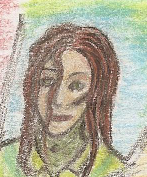
\includegraphics{sskreszta-portrait-alt-klein.png}\emph{Zu diesem
Abschnitt gibt es nur teilweise echten Aufschrieb (in
\href{http://1w6.org/deutsch/kampagnen/waechter-der-zeit/gedaechtniskristall/kerker-und-drachen}{Kerker
und Drachen} {[}11{]}). Daher erzählt hier direkt
\href{http://1w6.org/uzanto/drak}{Drak} {[}12{]}.}

Wir haben in den vorigen Abschnitten versucht, uns in eine
Hochsicherheitseinrichtung einzuschmuggeln. Kalem und Sskreszta wurden
erwischt, unsere DNA registriert (Kalem nannte sich eine Angestellte der
Gilde - was sich als großer Fehler herausstellte, denn die Gilde mag es
gar nicht, wenn man ihren Namen benutzt) und erstmal gefangengesetzt.

Dann haben wir uns mit roher Gewalt befreit, während Fox das Gelände
fast infiltriert hatte. Bis zum Kontrollzentrum konnten wir uns
vorkämpfen und wurden dann Zeugen, wie eine andere Gruppe Angreifer mit
einem schwarzen Schiff landete und ein fürcherliches Gemetzel
anrichtete. Kalem und ich flohen vor einem hummerähnlichen, Raketen
verschießenden und Psi-geschützten fast-Panzer in den Keller, haben drei
Tarnkapseln dort weglevitiert und sind nach oben entkommen.

Dort kämpften wir vor einer Lagerhalle mit einem Synachu und zwei
weiteren aus der Gruppe. Wir wurden fast niedergemacht, bis Fox mit
seinem Scharfschützengewehr eingriff. Dann warf Kalem eine Energiekapsel
und feuerte auf sie. Die Explosion verschaffte uns die Zeit zu fliehen -
und sie begann die Ära der explodierenden Energiekapseln, die mir später
noch tiefe Narben und Risse in meinem Psi-Schild einbringen würden - und
mehr als einmal unsere Leben retteten.

Seit diesem Tag sind eine Million Creds auf Kalems Kopf ausgesetzt (von
der Gilde) und eine halbe Million auf meinen, und unsere DNS ist als die
von Terroristen gespeichert. Von dem anderen Team wurde in den
Nachrichten nichts erwähnt, stattdessen wurde die vollständige
Zerstörung der Basis nur uns in die Schuhe geschoben.

\emph{(Das war gerade in einem Rutsch aus dem Gedächtnis - nach über
sieben Jahren. soviel also zu schlechtes Gedächtnis. Selektiv trifft es
wohl eher :))}

\emph{(und verdammt, war das ein Ritt!)}

\section{Ein Verlust im Subraum}

\emph{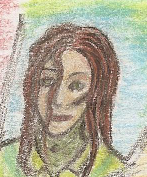
\includegraphics{sskreszta-portrait-alt-klein.png}°Sskreszta
schreit gequält auf. Dann sinkt sie nach vorne und ihr Kopf fällt auf
die breite Brust des Vogelmannes, der quer über ihrem Pilotensitz liegt.
Und trotz der schmerzverzerrten Züge liegt auf ihren Lippen ein leises
Lächeln, während der Brustkorb unter ihrem Kopf sich langsam hebt und
senkt.°}

Das ist eine Erinnerung an die ich gerne denke, auch wenn sie
schmerzhaft war. Heute werde ich meine Aufzeichnung sanfter führen und
meinen Kristall mit dem füllen, was passiert ist und was ich dabei
gefühlt habe, schließlich wird diese Aufzeichnung wohl keinen aus der
Flotte erreichen, und das sollte sie auch nicht.

Wir sind nicht mehr in dem Unterseeischen Hangar auf Styro, in dem unser
Schiff mit dem Tarnschild aufgerüstet werden sollte. Wir verließen ihn,
nachdem er angegriffen wurde. Unsichtbare Gegner tauchten auf. Als wir
sie erspüren konnten, waren sie schnell ausgeschaltet. Dann griffen uns
Space Marines an, waren aber den Schiffsgeschützen und meinem
Psi-Verstärker nicht gewachsen. Wir sind dann aus dem Hangar durch eine
dünne Wasserschicht geflogen. Kalem hatte die Hülle zum Glück bereits
wieder repariert, so dass wir durch kamen. Oben erwartete uns ein
interstellares Kampfschiff der Raumpatroullie, allerdings mit
deaktivierten Schilden. Der Pilot wird wohl seinen Job verlieren.

\emph{°Fox' Gleiter bricht aus der Wasseroberfläche. Direkt über ihm
füllt der düstere Schatten des Kampfschiffes den Himmel. Ohne
Verzögerung taucht der Gleiter wieder nach unten und jagt auf Höhe der
Wasserlinie davon. Ein Nebel aus Wasser füllt die Luft, als seine
Schilde das Wasser wieder berühren. Dann schießt Sskresztas Jäger aus
dem Windschatten nach oben, ein winziger Punkt gegen das interstellare
Schiff über ihnen. Der Jäger zuckt zur Seite, erreicht das Heck des
Schiffes und huscht zurück in den Windschatten des Gleiters. Augenblicke
später verstummen die Triebwerke des Kampfschiffes und es beginnt einen
immer schneller werdenden Sturz zu der Oberfläche des Sees.°}

Er hat versucht uns mit einem Traktorstrahl zu fixieren und so in
Reichweite zu halten. Zu unserem Glück hat er nicht gleich seine ganze
Kraft verwendet, ansonsten hätten wir kaum entkommen können. Er hätte
uns sonst mit in das Wasser hinein reißen können, was unsere gerade
reparierte Hülle wohl nicht lange ausgehalten hätte. Wer weiß, ob hinter
dem Fehler noch anderes steckte, immerhin sind auf Styros die Rebellen
aktiv.

\emph{°Ein Ruck geht durch den Gleiter. Er wird langsamer und die
Sensoren des Cockpits leuchten auf. Einen Augenblick später füllt ein
Schwarm Raketen die Luft über ihm, während er nur Meter über der
Wasseroberfläche entlang rauscht. Plötzlich taucht er etwas tiefer, und
feiner Nebel schießt in die Höhe, wo sein Rumpf den See berührt. Seine
Geschütze feuern und Raketen explodieren in der Luft. Durch die
Explosionen fliegt Sskresztas Jäger auf einen Punkt am Bug des Schiffes
zu, wo Fox in Sskresztas Cockpit die Quellen des Traktorstrahlt
aufstrahlen lässt. Drei kleine Explosionen glitzern auf der Hülle des
Schiffes auf. Dann schießt der Gleiter wieder nach vorne, als der
Traktorstrahl ausfällt. Augenblicke darauf berührt das Kampfschiff den
See und eine Wasserwoge rollt auf den Gleiter zu, während ein riesiger
Rumpf das Wasser des Sees verdrängt.°}

Wir flohen vor den Schiffen und wurden von 5 Stellarjägern angegriffen.
Ich versuchte mehrfach in ihren Geist einzudringen, aber sie hatten sich
jedesmal wieder unter Kontrolle, bevor ich etwas bewirken konnte. Kalem
saß an unseren Geschützen, während Fox Ausweichmanöver flog und ich im
Psi-Jäger die Angriffe der stellaren Jäger ignorieren konnte, da sie für
meinen Gefahrensinn bereits Sekunden im Voraus erkennbar waren.

Ihnen folgen allerdings 8 weitere, und als wir überlegten, ob wir uns
ihnen stellen sollten, berührte Etaros meinen Geist, ohne dass ich ihn
hätte eindringen spüren. Er gab uns Koordinaten, und wir machten uns
sofort auf den Weg.

Unterwegs griffen uns 16 kleine planetare Abfangjäger ab, von denen ich
die Hälfte im Gebirge vernichtete, während Kalem die Reichweite der
Geschütze ausreizte, um sie zu erreichen.

\emph{°6 Jäger fliegen eine weiter Kurve um einen Berggipfel. Direkt auf
der Flanke des Berges sitzt Ssksresztas Jäger unter einem Felsvorsprung.
Plötzlich gerät einer der Jäger ins Taumeln und vor dem Inneren Auge
Skresztas fließt Blut aus dem zerquetschtem Brustkorb seines Piloten
über die Konsolen im Cockpit. Als sich die Abfangjäger dem Felsvorsprung
zudrehen, wirbelt Schnee auf und der Psi-Jäger verschwindet nur
Augenblick darauf auf der anderen Seite des Hügels. Noch während die
Raketen den Felsvorsprung zerreißen, gerät der nächste der Abfangjäger
ins taumeln. Augenblicke darauf ziehen die Wände eines Gebirgstals an
Sskreszta vorbei, als ihr Psi-Jäger wieder am Heck des Gleiters von Fox
schwebt.°}

\emph{°Der Psi-Jäger fliegt in eine Höhle und hält abrupt vor der
Hochgewachsenen Gestalt Etaros'. Ein immer wieder hell flackernder
Psi-Schild umgibt den Vogelmenschen wie auch den Jäger, und Etaros
bleibt still stehen, als ein Überschallknall die Stille in der Höhle
zerreißt. Die Tür des Jägers fällt auf und Sskreszta wendet ihren Kopf
nach hinten. Wieder läuft ein Prickeln über ihre Haut, als die Präsenz
von Etaros sie einhüllt. Er faltet seine Flügel und tritt mit langsamen
Schritten in den Jäger. Sskresztas Augen hängen an seiner Gestalt. Ihre
Glieder scheinen gelähmt, ihre Lippen unmöglich zu öffnen. Dann nickt er
kurz. Sie wendet ihren Blick mit schwachem Zögern auf den
Hauptbildschirm und der Jäger schießt aus der Höhle. Die Luft in der
Höhle erzittert unter einem zweiten Überschallknall. Dann herrscht
Stille. Kein Laut dringt in die Höhle, und ganz langsam kehrt wieder
Ruhe ein. Dann lässt ein dritter Überschallknall Steinbrocken aus der
Decke brechen. Sskresztas Jäger steht erneut in der Mitte der Höhle und
verlässt sie einen Wimpernschlag später wieder mit 12 Sprungkartuschen,
die ihm hinterher schweben.°}

Ich habe die Kontrolle über meine Visualisierung weiter verloren als ich
dachte. Nachdem wir Etaros an Bord hatten, versuchten wir den Planeten
zu verlassen. Als wir die Scanner aktivierten, erkannten wir ein
Impulsnetz, dass den gesamten Planeten umspannte und uns eine Flucht
fast unmöglich machte. In der Kantine hatte dann Antov die Idee, das
Impulsnetz mit einem Psi-Schild zu schwächen, so dass wir durchbrechen
könnten. Um auf die nötige Geschwindigkeit zu kommen, beschleunigten wir
direkt oberhalb der Atmosphäre. Nach einer Stunde flug um den Äquator
zog Fox den Bug etwas nach unten, und wir prallten von der Atmosphäre
nach oben auf das Impulsnetz, um es an seiner schwächsten Stelle zu
durchstoßen.

\emph{°Verschiedene Kleinteile im Frachtraum reißen sich aus den
Verankerungen, als der Gleiter von der Atmosphäre in die Leere
geschleudert wird. Sskreszta lässt ihren Geist zu dem Impulsnetz
wandern, spürt den Flugweg des Gleiters. Sie greift in das Netz und
schafft einen von einem Schild umgebenen Kanal. Die Trajektorie des
Gleiters steigt, dann flucht sie. Die Darstellung des Impulsnetzes füllt
den gesamten Schirm, als sie ihren ersten Schild fällen lässt und erneut
ausgreift. Einen Augenblick später fliegt die Gleiter in den
geschaffenen Kanal. Anzeigen flackern, zeigen den
Geschwindigkeitsverlust, zeigen den Weg durch das Impulsnetz. Dann löst
sich der Gleiter aus dem Netz und die Sensoren eröffnen den Blick auf
die Weite des Alls. Und auf eine kleine Armada der Raumpatroullie.°}

\section{Was fehlt}

\emph{Das sind die Spielabende, zu denen wir wirklich keine echten
Aufschriebe haben. Sie bilden den Abschluss von
\href{http://1w6.org/deutsch/kampagnen/waechter-der-zeit/sskresztas-gedaechtniskristall/kampf-den-goettern}{Kampf
den Göttern} {[}13{]} und den Übergang zur
\href{http://1w6.org/deutsch/waechter-der-zeit/aufzeichnungen/sskreszta/piratenjagd}{Piratenjagd}
{[}14{]}. Insgesamt umfassen sie etwa 5 Spielrunden. Ich hoffe, ich
konnte die essenziellen Ereignisse hier zusammenfassen.}

\begin{itemize}
\item
  Durch die verbotene Zone. Kalem wird rausgerissen (durch das Jungh Ei,
  oder wegen ihm?). Sskreszta folgt ihr als Psi-Projektion: Bei dem
  Xynoc-Schiff trifft sie auf ein rotes Auge - und Kalem. Flucht zurück,
  mit Kalem.
\item
  Xynoc Schiff: Außen: Ebenen. Innen: Mehrere durch Gänge verbundene
  Räume. Fox kann sie durch sein Subraumgespür finden. Hieramel
  angekettet und in zwei Dimensionen geteilt. Fox schafft es im
  Kontrollzentrum, die Dimensionen zu verbinden. Spürt ankommende
  Sprünge: Rote Augen. Flucht raus. Mit unserer Gauss-Kanone aus dem
  Schiff die Xynoc beschäftigt. Protektor folgt uns: Rotes Auge.
  Protektor packt Kalem. Sie altert und bricht zusammen. Er packt
  Sskreszta. Dann erwischt ihn jemand (Fox? Etaros?). Sprung weg. Etaros
  bekommt von Kalem das Jungh-Ei auf die Brust gesetzt, um Etaros und
  Hieramel wieder zu verbinden. Das Ei verbindet sich mit ihm. Er wacht
  nicht auf. Aus ihm hervorpeitschende weiße Tentakel brechen durch
  unser militärisches Medkit. Viel Betäubung kriegt ihn ruhig.
\item
  Ruhepause:
  \href{http://1w6.org/deutsch/kampagnen/w-chter-der-zeit/orte/llovara}{Llovara}
  {[}15{]}. Auf Karren zum größten Tempel. Kyrië wiedergesehen: Ist
  Hohepriesterin und kämpft einen verdeckten Kampf gegen den Glauben an
  die Göttin (Sskreszta) und für Rationalität. Ein Jahr vergeht. Andere
  Reiche greifen sie an. Wir greifen ein, um die Stadt zu retten und
  zerstören damit Kyriës Erfolge („die Göttin greift ein``).
\item
  Seltsame Verwerfungen treten auf. Fox entdeckt eine Zat-Basis in einem
  dimensionsverschobenen Teil des Planeten. Wo in unserer Ebene einfach
  Terraner leben, existiert dort eine rapide wachsende Zat-Basis. Die
  Zat werden immer stärker und der Planet wird Stück für Stück
  vereinnahmt. Die Verschiebung löst sich auf und die Dimension mit Zat
  überdeckt die mit Menschen. Erdbeben erschüttern die Stadt. Wir
  fliehen, und diesmal kommt Kyrië mit. Der Boden draußen wird dunkel
  und bricht auf. Zat steigen daraus hervor und stürmen heran.
\item
  Fox ruft das Schiff. Ein Berobter taucht auf. Jodi Crown - ein
  Schatten der Vergangenheit \emph{(mein Charakter in der vorhergehenden
  Runde - noch aus der Schulzeit - und früherer Freund Sskresztas, der
  vor 6000 Jahren seine Existenz für ihr Leben gab und damit ihren 6000
  Jahre dauernden Kälteschlaf bewirkte. Er ist damals wohl doch nicht
  gestorben, aber irgendetwas ist passiert\ldots{})}. Er droht Sskreszta
  mit dem Tod. Wir kommen in letzter Sekunde in den Frachtraum. Etaros
  verändert sich. Weiß leuchtende Tentakel brechen aus ihm hervor und
  seine Psi-Kraft steigt ins Unermessliche. Er zwingt Sskreszta, sich
  zwischen ihm und Kyrië zu entscheiden. Sie entscheidet sich für Kyrië
  und wirft Etaros' Amulett aus dem Frachtraumtor. Kyrië stirbt. Etaros
  kämpft gegen den Berobten und wird schwer verletzt. Sskreszta geht
  nochmal raus. Fox schneidet mit dem Schiffsblaster durch Zat. Sie holt
  Etaros und das Amulett wieder rein („du wirst sie wiederholen``). Ein
  Zat-Schwarm beginnt sich zu manifestieren. Subraumkanäle öffnen sich.
  Kyrië steht wieder auf, wacklig, aber am Leben. Fox springt. Kyrië
  stirbt erneut. Sskreszta bricht zusammen.
\end{itemize}
Ab hier geht es weiter mit dem allzu realen Traum
\href{http://1w6.org/deutsch/welten/raumzeit/geschichten/piraten-und-zerg}{Piraten
und Zat} {[}4{]} und danach dem Kapitel
\href{http://1w6.org/deutsch/waechter-der-zeit/aufzeichnungen/sskreszta/piratenjagd}{Piratenjagd}
{[}14{]}.

\emph{Und mit diesem letzten der Texte vom Anfang unserer Reise ist das
gesamte
\href{http://1w6.org/deutsch/kampagnen/friedenszwang/aufzeichnungen/sskreszta-log}{Sskreszta-Log}
{[}10{]} online. 10 Jahre Spiel auf etwa
\href{http://1w6.org/print/book/export/html/59}{100 DinA4-Seiten}
{[}2{]} (chronologische Version), manches nur in Stichworten,
hauptsächlich aber als Geschichten. Ich hoffe, es gefällt euch!}

\section{Piratenjagd (Kapitel)}

Wir suchen die Piraten Gaia und Njillnor aus
\href{http://1w6.org/deutsch/welten/raumzeit/geschichten/piraten-und-zerg}{Piraten
und Zat} {[}4{]}, einem gemeinsamen Traum von Sskreszta und Kalem, um
mit dem Zat-Stab, den sie aus einem alten Tempel entwendet haben, Kyrië
wieder ins Leben zurück zu holen - Sskresztas tote Freundin, die während
dem größten Teil der Handlung in der Kryokapsel ihrer Kabine im Schiff
liegt.

\section{In der Tiefe der Baustation}

Wir sind mit den Gräbern nach unten, um zu prüfen, ob die Piraten dort
waren.

Dort bauten wir eine Woche lang ab und brauchten je drei Tage herunter
und hoch.

Am letzten Tag fand Fox einen zerstörten Bohrer. Ich ging gegen den
Protest der Leiterin runter und untersuchte ihn (es gab nur einen
Bohrer, der so tief kam. Wir mussten einen Ixitirit ausschalten, um ihn
nutzen zu können).

In dem Bohrer war eine Kiste. Als ich sie telekinetisch beührte,
explodierte sie. Vorher hatte ich noch den anderen Bohrer anbohren
müssen, damit ich nahe genug an die Kiste herankam (2m dicke Wände).

Mein Bohrer hing nach der Explosion plötzlich nur noch an seinem Kabel
und schwamm in flüssigem Stein. Ich konnte ihn langsam hoch schieben.

Vielleicht was es das Artefakt der Piraten, ich bezweifle es aber.

Wieder oben gingen wir in's Hotel zurück. Ich erwachte am nächsten
Morgen, weil ich von Feuer geträummt hatte.

Wir gingen um die Station herum. Auf der anderen Seite wurde ein Teil
der Außenhülle aufgeschweißt, und eine Polizeieinheit (wenig
Kampferfahren, sie fürchteten sich vor Schüssen) sprang hinein. Dabei
hat mich ein Psioniker berührt und wir hatten kurzzeitig fast Vakuum
(die Klimaanlage pumpe aus).\\ Wir konnten (hoffentlich) unerkannt
entkommen.

Das Hotel hatte gebrannt.

Am nächsten Tag sind wir zum Leiter der Sicherheit, ein Synarchu, der
uns nichts zum verschwundenen Mädchen sagen konnte und die
Geistergeschichten der Arbeiter für Humbug hielt. Er wollte mich
registrieren, und als ich mich weigerte legte er fest, dass wir nur
Starterlaubnis bekämen, wenn ich registriert wäre.

Wir verließen die Ebene, um uns das Gefängnis anzusehen und gingen dafür
zum Lagerraum, der direkt über den Zellen lag, in denen der Vater des
verschwundenen Mädchens gestorben war. Wir wollten vom Lagerraum aus die
Zellen mit ESP durchsuchen.

Im Lagerraum wurden wir mit Granaten beworfen, die ätzendes Gas
ausströmten. Wir versuchten die Angreifer erst zu finden, und als es uns
nicht gelange, flohen wir aus dem Raum in einen Gang, um mit dem Aufzug
runter zu gehen.

Als Fox, Antov und ich im Aufzug waren, stürzte der Aufzug nach unten.
Ich stieß die obere Klappe auf und sprang raus. Fox und Antov
verschwanden nach unten, und ich fing mich an einer weiteren Aufzugstür
im Schacht ab. Der Aufzug verschwand nach unten.

Später erst trafen wir uns wieder.

\section{Kämpfe in der Tiefe des Planeten}

Ich zwang eine Tür im Aufzugsschacht auf und lief durch den Gang
dahinter.

Nach kurzem hörte ich an einer Biegung die Stimme eines Mädchens und
folgte ihr. Sie verschwand im Gang dahinter, und ich rannte ihr
hinterher.

Der Gang führte mich in die Tiefen der Station. Weiter hinten neigte er
sich immer mehr dem Gravitationszentrum zu, und Nebel erfüllte ihn. Dann
sah ich einen SChatten im Nebel, mein Blaster schoss hoch, und ein
Geschoss jagte durch den Gang, verfehlte die gestalt jedoch. Im nächsten
Moment schälte sich dort Kalems Körperpanzer aus dem Nebel. Ich rief sie
an, und sie hielt ihr Feuer zurück. Vermutlich hatte sie mich schon
vorher erkannt.

Wir blickten den Gang hinunter und hörten das Mädchen schreien. Im
gleichen Moment spürte ich einen SChuss und trat zur Seite.

Eine unsichtbare Sonde griff uns an, Krallenspuren jagten über die
Wände, durchdrangen Kalems Schild und zerkratzten ihre Rüstung. Im
nächsten Moment wurde die Drohne von Kalem mit einem einzelnen
Blindschuss außer Gefecht gesetzt.

Dann fanden wir das Mädchen wieter hinten im Gang, wo die Schwerkraft
ausgesetzt hatte. Kalem holte sie, beruhigte sie und wir gingen zurück
in den Aufzugsschacht,um nach oben zum Shuttle zu kommen.

Kalem zog mich in dem Aufzugsschacht nach oben, als plötzlich Neben
auftauchte, und eine Salve Geschosse ihren frischn geladenen Schild
traf. Ich stürzte, fing mich an einem Zwischengeländer ab, und spürte
erneut schmerzhaft, wie viel mir verloren geht, weil ich mich mit meinen
Kräften selbst nicht erreichen kann.

Dann feuerten wir auf den Angreifer, der sich im Nebel verborgen hielt.
Meine Schüsse gingen weit vorbei, doch kalem gelang ein treffer. Ich
trat zur Seite, als ich spürte, dass gleich eine Salve Schüsse dort
einschlagen würde, wo ich gerade stand, dann ging ich zum Rand und ließ
mich auf die eins tiefere Wartungsebene fallen.

\emph{°Kalem schwebt am Rand des Schachtes. Plötzlich taucht vor ihr ein
schwer Gerüsteter auf, seine Faust schießt vor und zerschmettert ihren
Schild. Einem zweiten Schlag weicht Kalem aus. Sie packt den Angreifer
und schleudert ihn in die Tiefe, doch noch im Fallen schnappt seine
Faust zu und entreißt Kalem das Mädchen.°}

Er verschwand nach oben, doch wir feuerten beide, und Kalems Schuss traf
ihn schwer. Etwas weiter oben fanden wir das Mädchen tödlich verletzt
auf einem Geländer. Ich versuchte sie zu heilen, doch meien KRaft
reichte nicht, also zog ich mein Medkit aus der Panzerung und schloss
sie an.

Wir verließen die Station ungestört mit dem gepanzerten Shuttle und
trafen dabei Fox und Antov wieder. Unser Schiff konnte nach kurzem
Bequatschen der Verantwortlichen Wache starten, auch wenn ihm das Ärger
vom Sicherheitsoffizier einbringen wird, da ich nicht registriert wurde.
Ich plane auch, mich weiterhin nicht registrieren zu lassen.

Dann machten wir uns auf den Weg.

Nach den zwei verlorenen Wochen wollten wir eine Abkürzung durch den
Nebel nehmen.

\section{Gefangen (in Zeit und Raum)}

Nach dem Sprung wachte ich in meiner Kryokapsel auf. Der Computer
meldete mir auf Anfrage, dass Kalem an Bord sei, Fox aber das Schiff
verlassen hätte.

\emph{° Stille herrscht in dem leeren Gang des Schiffes. Das Kom knackt
und Sskresztas Stimme hallt von den Wänden zurück.}

\emph{``Fox? Fox? Hörst du mich? Bitte Antworten!''}

\emph{Nur Stille antwortet. Selbst der Schiffsantrieb ist verstummt. °}

Nach einem kurzen Essen machten wir uns auf die Suche nach ihm.

\emph{° Kalem tritt aus dem Schiff. Sskreszta folgt ihr, und hinter dem
Schott des Schiffes öffnet sich der Blick auf einen stählernen Hangar,
in dem ein einsamer Warpgleiter auf drei Stelzen steht. °}

Wir durchsuchten den Hangar und aktivierten die Terminals. Auf einem von
ihnen fanden wir einen PDA mit Karten und Codes von Fox. Dann
betrachteten wir den Gleiter. Er öffnete sich uns nicht, und in seiner
Mitte war ein Punkt, den meine Psionischen Fühler nicht erreichen
konnten, ein wießter Fleck für mein Psi.

\emph{° Sskreszta tritt zu dem Jäger. Langsam erweitert sich ihre
Wahrnehmung. Sie spürt, wie ihre geistigen Fühler durch die Wand des
Schiffes gleiten, über stählernen Boden und immer Tiefer in's Innere,
wie sie es erkunden, bis jeder Winkel des Innenraumes vor ihrem
geistigen Auge entstanden ist und ein Bild des Gleiters formt. Doch tief
im Herz des Bildes liegt eine Leere. Teif im Inneren, dort wo der
Antrieb sein sollte, ein Punkte, an dem ihre Fühler abgleiten wie von
geöltem Glas, einer Sphäre, die Sskreszta weder packen noch in sie
eindringen kann. Plötzlich verschwindet das Bild und Sskreszta schüttelt
den Kopf. ``Da ist etwas, aber ich kann es nicht greifen.'' °}

Nachdem wir es auch nicht schafften, ihn ohne Gewalt zu öffnen, ließen
wir ihn erstmal stehen und verließen den Hangar durch den linken von
zwei Ausgängen.

Nur wenige Schritte tiefer im Gang sahen wir uns einer massiven Wand aus
Eis gegenüber, die erst ein Blasterschuss zertrümmerte. Dahinter fanden
wir eine Abzweigung, und die Tür zum Kontrollraum 2. Sein Türschild
verriet uns den Namen. Mit den Codes von Fox konnten wir ihn öffnen und
fanden dort mehrere Sicherheitsterminals und noch einen PDA von Fox. Er
enthielt weitere Codes und die Pläne der gesamten Station.

*° Das Licht der Monitore flackert. Plötzlichn erfüllt eine Kinderstimme
den Raum:

``Ihr seid hier falsch. Geht wieder.''

Die Stimme verklingt, dann erscheint neben Kalem und Sskreszta das
flackernde Bild eines kleinen Mädchens.

``Was macht ihr hier?'' °*

Zwei Gänge führten auf eine Plattform, von der aus ich mit einem
Schwebewagen über ein Eisfeld und unter einem Himmel voller Eiszapfen zu
Asteroid Nummer 3 auf eine ähnliche Basis kam. Wir fanden dort zwei
weitere PDAs und den Energiekern der Station (an den wir mit Fox' Codes
rankamen).

Wie sahen ihn aber nur kurz an und gingen dann zu Basis 2. Auf dem Weg
dorthin erkannten wir, dass die Eiszapfen an der Decke gewachsen waren.
Dann und wann stürzten sie in die Tiefe.

In Basis 2 fanden wir einen weiteren PDA von Fox mit Infos, dass er hier
die Forscherräume gefunden hätte.

Als erstes stießen wir allerdings auf einen Hangar, in dem ein Roboter
auf Schwebedüsen seinen Wachgang schob.

Wir ignorierten ihn nach erstem Schrecken und sahen uns weiter um.

In einem weiteren Gang fanden wir leere Schlafquartiere, die erst
kürzlich verlassen wirkten und nicht aufgeräumt waren. In einem der
Betten lag ein Toter, wir konnten allerdings außer dem Ausdruck des
Schreckens auf seinem Gesicht keine Todesursache erkennen.

Hinter der zweiten Tür war die Forschungsabteilung, mit Terminals,
ungeräumten Schreibtischen, und auf einem der Stühle einer Frau in
weißem Kittel, in deren Gesicht sich tiefstes Grauen eingegraben hatte,
die jedoch kein Zeichen der Verwesung zeigte.

Bevor wir dort weitersuchten, gingen wir in die Tür am Gangende, die wir
mit Fox' Codes öffnen konnten. An der Konsole dort saß ein
Wissenschaftler, auch der mit dem Ausdruck des Schreckens auf dem
Gesicht und lange tot, aber eingeloggt.

Wir nutzten sein Terminal, um Daten der Station zu erhalten, bis
plötzlich die KI neben uns stand, in Gestalt des Mädchens ``Lyra''. Sie
fragte uns, was wir machten, und nachdem wir herausfanden, dass es eine
Subraumbarriere gab, die nur aus dem Kontrollraum in basis 1 zu lösen
war, und für die wir die Schlüssel fanden, gingen wir wieder raus. Lyra
begleitete uns.

Die Frau, die tot im Forschungsgereich saß, nannte Lyra ihre ``Mutter'',
als wir sie fragten, wer es sei, und wir fanden Käfige mit
Versuchstieren, und natürlich Computer und Tech, aber das war für uns
kaum wichtig.

Wir wanderten durch die Station, das Schiff verschwand aus einem Hangar
und tauchte im anderen auf, wir wurden von einem Roboter mit
Gravitationswaffen getoetet und wachten unverletzt wieder auf. Ein
Psi-Wesen, das wie ein Kind sprach, saugte mir einen groszen Teil meiner
Kraft aus, und es erschien uns in der Gestalt der verletzten Kyrie, die
ich zu heilen versuchte. Als ich zusammenbrach gab Kalem ihre ganze
Kraft und riskierte ihren eigenen Tod, doch es war nicht Kyrie, die wir
heilten.

Kalem begann dann ploetzlich zu fauchen wie ein Zergling, riss die
Kontrollraumtuer auf und verschwand schlagartig.

Zwischendrin trafen wir Fox wieder, liefen ueber die Auszenseite der
Station (die Teils in einem in drei Stuecke gebrochenen Meteoriten war),
sahen dort Zerg, schalteten vom Kontrollraum aus den Strom aus (Etaros
meldete sich ueber einen PDA und sagte uns, wir sollten es tun), so dass
die Subraumsperre zerfiel.

Kalem lag im Schiff, als wir wieder gestoppt wurden. Sie wachte
auf,waehrend psionische Blockaden entstanden.

Ich sprang raus, doch ich hatte kaum mehr Kraft seit das Psi-Wesen mich
ausgesaugt hatte und konnte nur hilflos zusehen, wie Eis die Station
ueberzog.

Dann blitzte eine Erinnerung in meinem Geist auf: Jodi Crown, der sich
über mich beugte.

\emph{° Ein Gesicht, scharfe Gesichtszüge und irisierende Augen, ein
zartes Lächeln, dann berühren sich Lippen. Wärme und ein Beben im
Inneren breiten sich aus.}

\emph{``Ich für sie'' °}

Im gleichen Moment erkannte ich um mich und an mir Stränge und Fäden aus
psionischer Kraft. Ich riss mein Psi-Schild in die Höhe und spürte
erneut meine ganze Kraft, und mehr. Ein warmes Gleißen erfüllte mich,
und es zerschnitt mühelos die Fäden, die mich gefangen gehalten hatten.

Ich konzentrierte mich auf die Bilder von Jodi und rief auch die Bilder
von Kyrie hervor, von den schönen Zeiten auf Llovara, und das Gleißen
nahm zu.

Gleichzeitig spürte ich Gestalten um mich, Wissenschaftler, alle mit
leuchtenden Fäden an ein Wesen gebunden, das ich nur als Lichtschimmer
sah und das selbst nicht allzu stark wirkte.

Ich versuchte einmal, alle Faeden gleichzeitig zu zerreißen, doch dafür
reichte meine Kraft nicht. Also befreite ich die Wissenschaftler
einzeln. Kaum hatte ich den ersten losgeschnitten verschwand er und die
anderen wurden real. Wo sie standen wuchsen sich bewegende Statuen aus
Eis aus dem Boden, die versuchten mich anzugreifen.

Im nächsten Moment sprangen die Schiffslaser an und Kalem eröffnete mit
ihrer Stabwaffe das Feuer auf die Eisgestalten.

Wären Kalem und Fox nicht gewesen, wäre ich dort gestorben, doch so
levitierte sich Kalem zu mir, ich fluchte einmal wieder, dass ich zwar
tonnenschwere Lasten heben, aber mich selbst nichtmal anstupsen kann,
und sie trug mich in's Schiff. Beim Abflug meldeten unsere Sensoren,
dass ein riesiger Eisbrocken, der fast schon die Station umhüllt hatte,
schnell schrumpfte. Wir sind sicher, dass dort Etaros war. Dann
aktivierte Fox den Sprungantrieb.

Es war viel zu früh für einen kontrollierten Sprung, doch er sagte, in
der plötzlich wieder existierenden Sprungbarriere sei ein Riss, der sich
gerade schließen würde, und er hätte nur diesen Moment. Wir sagten ihm
er solle springen und schafften es gerade noch in die Kryokapseln.

Nach dem Sprung erwachten wir wieder und fanden Fox schwer verletzt im
Cockpit, nachdem die Spannungen im Subraum ihn fast zerrissen hatten.

Stichwörter: Mit Etaros Blick in die Vergangenheit des PDAs versucht
-\textgreater{} Fast gefangen, Verschlüsselung in der Zeit.

Etaros sagte, dass es eine Chance für Kyrie gibt: Die Jungh.

Es schien ihm sehr schwer zu fallen.

\section{Ranmex, Tempel und Schatten}

\emph{°Dunkle Schatten stürzen aus dem Himmel.}

\emph{Dunkle Schatten steigen aus dem Waldboden.}

\emph{Ein Schatten schwebt in der Luft, ein rotes Stielauge öffnet sich
weit.}

\emph{Eine grauschwarze Hand hebt sich.}

\emph{Die Zeit fließt wie träge Masse.}

\emph{Ein Sog entreißt das Leben und Haut und Knochen werden brüchig und
schwach.°}

Raus!

Dieser Eintrag ist für mich. Die Raumflotte wird ihn sowieso nicht mehr
lesen und welche Nachwelt sollte sich schon für uns interessieren, wenn
wie hier mitten im Sturm der Zerg von Protektoren ausgelöscht werden?

Aber ich schreibe jetzt seit Jahren, und ich werde nicht einfach
aufhören, nur weil ich durch Kalem die Rufe der Zerg gehört habe und
dieser ganze Planet gegen uns steht und Fox für einen Verräter an deinem
Clan hält. Und er ist jetzt tot, auch wenn sie ihn nicht angerührt
haben.

Es sah noch gut aus, als wir auf der Außenstation von Ashar gestartet
sind.

``Faria'', die Abgesandte des D'sol Clans, hatte uns offiziell
angestellt, um dem Transporter des Clans Geleitschutz zu geben, und auf
der Meteoriten der D'sol haben wir Kontakt zu 3 Zergwissenschaftlern
bekommen, die uns als Wachen und Pilot für ihr Projekt in einem für
Wissenschaftler zugänglichen Tempel etwa 1000 km nördlich unseres Ziels
anstellten.

Vorher konnten wir auf der Station noch unser Schiff reparieren, nachdem
wir den Dockplatz eines Kapitäns erhielten, für den wir zwei seiner Crew
gerettet hatten, die bei einem Piratenangriff verletzt worden waren
(auch wenn wir noch immer nicht ganz sicher sind, ob sie nicht selbst
die Piraten waren).

Einem war der Großteil seiner Haut und Lunge verbrannt, dem anderen der
komplette Bauch aufgeschnitten.

Während ich mich um die Verletzten kümmerte, reparierte Kalem
Lebenserhaltungssystem, Hülle und GRavitationskontrolle des Schiffes.

Die Verletzten lagen beide in Kryokapseln, und der Körper des
Verbrannten reagierte gut auf meine Kraft. Seine Haut, Lunge und
verflüssigte Augen regenerierten sich, und er sollte schon in ein paar
Tagen wieder einsatzbereit sein.

Als ich mich nach seiner Heilung kurz entspannte und den Kapitän nach
Wasser fragen wollte, fand ich ihn in völligem Schockzustand im Cockpit.

Kalem heilte ihn, und als er wirklich realisierte, dass über die Hälfte
seiner Crew tot war, ließ ich ihn von seinem Medkit ruhig stellen.

Danach knackte Kalem seinen Bordrechner und gab mit Befehlszugriff.
Später passte ich dann die Berechtigungen so an, dass die Befehlsgewalt
automatisch an den Kapitän zurückgehen würde, wenn er wieder
handlungsfähig würde, und gab auch Kalem, Fox und Antov vollen Zugriff.

Dann kam Fox mit unseren Panzerungen und darin meinem Medkit, so dass
ich mich um den zweiten verletzten kümmern konnte. Um sicher zu sein,
dass seine gefährlichsten Verletzungen zuerst geheilt würden (seinen
aufgeschnittenen Darm), griff ich direkt in seine Bauchhöhle, schob die
zerschnittenen Darmteile zusammen und ließ erst dann meine Kraft
fließen. Sein Körper nahm die heilung weitaus schwächer an, als der
seines Schiffsgefährten, aber es genügte, um sein Leben zu retten. Seine
Organe sind wieder verschlossen.

Wieder auf dem Schiff erhielten wir die Bestätigung des Schutzauftrages,
wir mussten allerdings noch persönlich vorbei. Zusätzlich bekamen wir
das Angebot von 1,5 Millionen creds, wenn wir einen bestimmten
Forschungskomplex maximal beschädigen würden. Leider lag der Komplex
weit von unserem Ziel entfernt, und wir haben auch jetzt noch nicht
entschieden, ob wir annehmen.

Der D'sol Clan war deutlich auf Rache aus, denn sie wurden von dem Clan
``Kinder Thanos'' fast vollständig ausgelöscht, obwohl sie verbündet
waren.

Die ``Kinder Thanos'' experimentieren gerüchteweise mit Ranmex Biestern,
und später erfuhren wir, dass der D'sol Clan wohl starke Anlagen zu
Biestern hat.

Als wir Zwischenstation auf dem Meteoriten unserer Auftraggeber machten
udn mit ihnen aßen, kamen die ersten Probleme:

Sie hatten Fox erkannt. Da wir in ihrem Auftrag da waren, gab das
Clanoberhaupt Fox 12 Stunden, dann würde der gesamte Clan erfahren, wer
Fox ist. Unter den Ranmex gilt er als Abtrünniger im Exil, und viele
würden ihn gerne tot sehen.

Die Tochter des Clanoberhaupts hat ihn seitdem mit unverholenem Hass
behandelt, und als ich während eines Übungsfluges mit ihr im Cockpit
war, habe ich sie gewarnt, dass Fox mein Kapitän, Besitzer des Schiffes
und Teil meiner Crew ist, und dass ich sie auf der Stelle töten würde,
wenn sie ihn angreifen sollte.

Am Abend, noch vor Ablauf der 12 Stunden, waren wir in einer Disko und
Kalem hat getanzt, bzw. Kampfbewegungen an den Rhythmus der Musik
angepasst, während ich mich auf jede Gefahr für Fox konzentrierte.
Obwohl ich ein paar mal falsch reagierte und einmal einer der anderen
Gäste durch den Raum flog, als er aussah, als wollte er eine Waffe
ziehen, wurde Fox kein einziges Mal angegriffen. Das Clanoberhaupt hatte
wohl Wort gehalten, und niemand hatte Informationen rausgelassen.

Am nächsten Tag trafen wir auf die Zergwissenschaftler, mit denen wir zu
dem Tempel in der Nähe unseres Ziels kommen wollten.

Einer der Zerg war schlacksig mit vielen Armen, die ihm wie vergrößerte
Rippenbögen aus den Seiten wuchsen, der zweite ein psionisch begabter
Zergling und der dritte war fast menschlich, bis auf das zweite extrem
muskulöse Armpaar, das ihm aus dem Rücken wuchs und um seine normalen
Arme herum nach vorne ragte.

Sie alle trugen weiße Forscherkittel, und die Versuchung, ihr Aussehen
zu kommentieren war für uns alle kaum auszuhalten, aber es waren unsere
Arbeitgeber. Zerg in laborkitteln wirken sehr seltsam.

Wir kamen auf den Planeten und schmuggelten Etaros und unsere Waffen (4
meiner Blaster wurden gefunden. Ich hoffe, die zwei übrigen reichen -
einer ist während ich diesen Eintrag hier aufzeichne bereits an die
Schatten des Waldes verloren gegangen). Ich half Etaros unter der Plane
der schweren Geräte der Zerg bis zum Tempel zu kommen.

Im tempel setzten meine Augen fast aus. Er strahlte psionisch so massiv,
dass ich meine Kräfte blockieren musste, um überhaupt wahrzunehmen, und
ein Teil des Tempels schien nur psionisch zu existieren. Ich sah den
Teil und konnte ihn telekinetisch berühren, nicht aber körperlich.
Vielleicht kann es Kalem, wenn sie ihren Körper psionisch auflädt. Nach
Informationen von Etaros gibt es wohl auch Teile des Tempels, die nur im
Subraum existieren. Fox sollte sie wahrnehmen können.

Drei recht ereignislose Tage später entschieden die Wissenschaftler
endlich, dass sie nicht mehr auf, sondern unter dem Tempel forschen
wollten, so dass wir endlich in die Gänge kamen, mit denen wir hofften
zum anderen Tempel zu kommen.

Wir fanden in einem der Gänge mit den Wissenschaftlern eine
verschlossene Tür, bei der Fox Subraumschwingungen anregen konnte. er
sagte vorher, er würde eine Welle spüren. Kalem und ich steigerten das
psionische Abbild dieser Wellen auf meine Idee hin zu einer immer
stärkeren Welle. Als die Welle brach, hätte sie uns fast zerrissen. Wir
waren für Momente ohnmächtig, und die der Bruch hinterließ Wunden in
meinem Geist.

Kurz darauf rief uns Etaros. Er sprach aus größerer Entfernung so leise,
dass nur Fox ihn hörte. In einem Seitengang fanden wir ihn vor einer
weiteren verschlossenen Tür. Er war grausam geschwächt, als müsste er
ständig kämpfen, er nahm wohl zu viel wahr, und er sah alt aus, bis er
seine Flügel um sich legte und sich binnen Augenblicken verjüngte.

Fox starb bei dem Versuch, die Tür des Raums über den Subraum zu öffnen,
und es blieb nur eine Hülle von ihm. Alle inneren Organe sind
verschwunden, aber die Tür öffnete sich.

Wir brachten ihn \ldots{}

\emph{°Wellen durchziehen den Tempelraum.}

\emph{Er weitet sich, verengt sich, weitet sich erneut. Dann kippt er.}

\emph{Fox stürtzt zu Boden, Sskreszta springt zu ihm und fängt ihn bevor
er den Boden berühren kann.}

\emph{Fox ist zu leicht.°}

Raus! Ich hasse es, die Kontrolle über meine Visualisierungen zu
verlieren, und ich will nicht noch mehr daran denken!

Es war bereits früher morgen, als Kalem den PSI-Verstärker der Zerg an
mich angepasst und ich ihn heruntergebracht hatte, und wir entschieden,
erst am nächsten Tag zu versuchen den anderen Tempel zu erreichen.

Doch vor dem Rückweg blickte ich mit dem Psi-Verstärker in die zukunft.
In Kalems Weg sah ich Dunkelheit, die durch Licht ersetzt wurde. In der
von Etaros sah ich nichts als Schatten. Er verbirgt sie.\\ Als letztes
sah ich nach dem Weg, fand drei Motorräder und danach eine Vision von
Schatten, die vom Waldboden aus anderen Schatten aus dem Himmel
entgegentraten.

Etwas sagte uns dann, wir sollten nicht mehr los, und er und ich gönnten
uns etwas Entspannung.

Als ich aufwachte war er verschwunden, hatte aber eine Nachricht
hinterlassen: Wir sollten ihm nicht folgen. Aber dass wir ihn alleine in
den Tod gehen lassen kann er vergessen, und verdammt, ich hasse es,
morgens neben einer dampfenden Tase kaffee aufzuwachen!

Kalem und ich nahmen (d.h. stahlen) die zwei verbleibenden Motorräder,
unsere SchiffsKI ``Lyra'' knackte die Codes für uns und wir fuhren mit
mehr als 1000 km/h mit Autopilot los. OHne meinen alten Psi-Verstärker
geht auch mein Blick in die Zukunft nicht weit genug, um bei der
Geschwindigkeit zu steuern.

Wir waren nur noch ein paar Kilometer von dem anderen Tempel entfernt,
als die Schatten aus dem Himmel zu fallen begannen, sich als Protektoren
herausstellten und damit meine schlimmsten Befürchtungen bestätigten.

Der Rest des Fahrt ist verschwommen. Ich weiß noch, dass ich meinen
Geist mit Kalems verschmolzen habe, und dass mein Blick in die Zukunft
weit genug ging, um Protektoren treffen zu können. Ich wünschte, wir
hätten ``Future'' aus meiner alten Einheit dabei gehabt. Sie hätte es
mit den Protektoren aufnehmen können. Vielleicht wurde sie deswegen
ausgelöscht.\\ Am Ende verschwanden die Protektoren, als wären sie nie
da gewesen, und wir fuhren weiter zum Tempel.

Doch noch bevor sie verschwanden spürte Kalem den Ruf der angreifenden
Zerg, die sich dem Planeten näherten, und durch ihren Geist spürte auch
ich ihn.

In Sichtweite des Tempels traten uns die Schatten des Waldes entgegen,
einer davon ein riesenhaftes Monster. Dann hörten wir einen Schrei, der
wie Etaros unter schrecklichen Schmerzen klang, und etwas riss uns in
eine Halbwelt, in der wir immer älter wurden, je realer die Halbwelt
wurde, Haut und Knochen brüchig schienen und kaum Kraft im Geist
verblieb.

Wir sahen nur Nebel, aber ich fand Etaros. er lag auf dem Bauch, seine
Flügel über ihm, und kroch unter seine Schwingen, um zu sehen, ob er
noch lebte. Ich war überglücklich, als ich seinen Puls spürte.

Etwas brach in der Realität und wir erwachten auf weißen Betten. Ich war
froh, dass ich den Gedächtniskristall mitgenommen habe, und dass ich
zumindest die Kraft habe, diesen Eintrag aufzuzeichnen.

Was auch immer geschieht, es geht weiter, und wir werden sehen wohin.

\section{Aus der Zelle in den Kerker, Teil 1}

Als ich nach mehrfachem Erschöpfungsschlaf wieder erwachte, wandten sich
verschiedene Schläuche und Drähte von meinen Körper zu einem Punkt in
der Decke.

Ich war froh, dass ich keine Schmerzen spürte, wusste aber dass ich das
nur harten Drogen zu verdanken hatte.

Kalem lag auf einem Bett neben mir und war ebenso fast in Drähten
eingesponnen.

Schon der Versuch aufzustehen war anstrengend, und wir schliefen
mehrfach wieder ein bevor unsere Körper sich soweit erholt hatten, dass
wir auf eigenen Beinen stehen konnten.

Gleichzeitig hingen mit jedem Aufwachen weniger Schläuche an uns, und
ich träumte in jeder Nacht von einer dunklen Gestalt. Schon da glaubte
ich \emph{Aro} wiederzuerkennen.

Meine Psi-Kräfte kehrten ebenso zurück, doch ich bemerkte auch einen
Drogenport an meiner Seite, dessen Licht bei jedem Einsatz von Psi etwas
weiter vom Grünen ins Rote überging. Auf dem Tischchen neben dem Bett
(das fest in die Wand montiert schien) fand ich passende Drogenpatches,
und als ich sie zu ignorieren versuchte, erfuhr ich, dass es diese
Drogen waren, die die Schmerzen zurückhielten.

Als nur noch ein Draht an meinem Körper hing, im Nacken, schaffte ich es
zur Tür zu gehen. Die Tür öffnete bei Berührung ein Fach in der Wand, in
dem ein Pad eingelassen war. Auf Sprachbefehl zischte die Tür auf.

Wir waren in einem medizinischen Zellentrakt, dessen Wände psionisch
geschirmt. Hochsicherheit.

Die nächsten zwei Wachzeiten verbrachten wir mit dem Versuch, den Trakt
zu verlassen. Es waren ein gutes Dutzend leere Zellen, verbunden durch
einen Gang, der in zwei massiven Schotts endete, und wir hatten an den
Pads ungenügende Zugriffsrechte, um den Ort zu erfahren.

Am Ende gelang es mir, die geschirmte Glasscheibe vor einem der Pads mit
einem telekintisch beschleunigten Wassertropfen reißen zu lassen, so
dass Kalem sie vollends aufbrechen konnte.

Ich merkte auch, dass die Droge schneller aufgebraucht wird, wenn ich
Psi einsetze. Und ich muss lernen, mit meinen gewachsenen Kräften
umzugehen. Ich nutze immernoch meine Ausbildung aus der Raumflotte, aber
meine Kräfte sind seitdem um ein Vielfaches gestiegen. Meine
Feinkontrolle reicht lange nicht mehr aus, um sie effizient zu nutzen.

Die Patches hab ich mir mit abgerissenen Streifen des Krankenhauskittels
an Arme und Beine gebunden.

Nachdem das Pad aufgebrochen war, gelang es Kalem uns Sicherheitszugriff
auf die internen Systeme zu geben, so dass wir die Schotts öffnen
konnten.

Wir wanderten durch einen weiteren Zellengang, bei dem in einer Zelle
die Rückwand wie von Klauen aufgerissen war. Da es auch die Schirmung
der Wand durchbrechen musste, müssen dahinter enorme Kräfte gewesen
sein. Ich will dem Wesen nicht gegenübertreten, das hier gefangen war.

Das nächste Schott führte uns durch eine Schleuse in normale graue
Bereiche, durch einen Aufzug in eine demolierte Beobachtungskanzel, die
durch Kraftfelder getrennt war, und dort zu \emph{Aro}, der uns in
voller Panzerung entgegentrat.

Wir folgten ihm in seinen und \emph{Aikas} Unterschlupf, einen Raum, den
\emph{Aro} mit einem tonnenschweren Trümmerstück verschlossen hatte. Die
Servos in seiner Panzerung wären der Traum der alten Raumflotte gewesen.

Er legte die Panzerung ab und sein verbranntes Fell kam zum Vorschein.
Es sah ein Stück weit geheilt aus, aber weit weniger als ich es nach den
Monaten, die wir uns nicht gesehen hatten, erwartet hätte.

Dann kam \emph{Aika} von einem Erkundungsgang zurück. Ich verstehe
immernoch nicht, wie das System Kinder für seine Aufträge nutzen kann,
aber zumindest von ihren Fähigkeiten her überflügelt sie die meisten
Erwachsenen.

Wir erholten uns kurz, dann ging Aro auf einen Erkundungsgang und ich
folgte ihm den ersten Teil. Er begleitete mich wieder zurück, bevor er
weiterging. Das Trümmerstück vor dem Unterschlupf wäre mir selbst mit
ganzer Kraft zu schwer gewesen, und meine Psi-Fähigkeiten waren
immernoch nicht wieder ganz zurückgekehrt.

Später gingen Kalem und Aika zu einem der Kontrollzentren, um sich ins
Computersystem des Komplexes zu hacken. Bevor sie zurückkamen brach im
Unterschlupf die Hölle los.

Aro wurde schwer von Gaußgeschossen getroffen, wir sprengten den
Unterschlupf, dann flohen wir durch einen Wartungsschacht, den ich mit
einem Blaster im Selbstzerstörungsmodus unter uns verschloss.

Ich hob Aro durch den Gang nach oben und kletterte dann selbst eine gute
Stunde die Leiter hinauf, bis ich völlig fertig ankam. Das sind die
Momente in denen ich Kalem darum beneide, dass ihr sie ihre Psi-Kräfte
auch auf sich selbst richten kann.

Oben angekommen, versuchten wir vom Komplex in den umliegenden Wald zu
fliehen. Etwas zog mich in den Wald in Richtung Tempel. Nach wenigen
Schritten wurden wir aber von einem Panzer aufgehalten und es gelang mir
gerade noch Aro von mehreren tödlichen Treffern durch Kampfdrohnen des
Panzers zu heilen und die Erde unter uns aufzureißen um uns zu
verbergen, bevor ich ohnmächtig zusammenbrach.

Als ich erwachte stand der Wald in Flammen und der massive Fels hinter
dem wir in Deckung geflohen waren lag in zwei Stücke geborsten. Von dem
Panzer war keine Spur zu sehen. Aro blieb ohnmächtig, und ich spürte
keinerlei Sog mehr vom Tempel.

Die nächsten Stunden sind eine verschwommene Mischung aus Erschöpfung,
Schmerz und Durst. Ich trug Aro durch den brennenden Wald, während immer
wieder Hitzestöße durch die Risse in meinem Psi-Schild drangen und meine
Kraft immer weiter erstarb.

Eine Nacht verbrachten wir in einer Grube, die ich im Waldboden aushob,
dann ging der Weg scheinbar endlos weiter.

Doch irgendwann sah ich die riesigen Flammen am Rand des Brandes und wir
kamen hinter ihnen auf noch grüne Wiesen. Ich riss den Boden viele Meter
tief auf, bis Grundwasser in die Grube sickerte. Dann hob ich das Wasser
heraus und trank, und gab auch Aro zu trinken, soweit ich es in seinen
Mund bekam.

Als ich ihm Wasser ins Gesicht schüttete schien er endlich zu erwachen.
Seine Augen zuckten und ein Grollen entwich seiner Kehle. Als er sich
langsam auf vier Beine aufrichtete und sein Blick meinen traf wusste
ich, dass die Erzählungen über Ranmex Bestien wahr sind.

Sein Körper begann zu wachsen und seine Augen schienen zu glühen,
während er langsam auf mich zutrat.

\emph{° Dumpfes Grollen lässt den Boden erbeben. Das Feuer der Raserei
brennt in dn Augen des Ranmex inmitten des schwarz verkohlten Fells
seines Gesichtes. Seine Krallen graben sich in den Boden, als er sich
Sskrezta langsam nähert.}

\emph{Sskreszta tritt einen einzelnen Schritt zurück. Das einst weiße
Krankenhaushemd hängt in verbrannten fetzen um ihre Schultern und die
feinen Schuppen auf ihren Körper sind trocken aufgesprungen und
stellenweise verkohlt und schwarz wie Aros Fell.}

\emph{``Beruhige dich Aro!''}

\emph{Er kommt näher, dann beginnt er Sskreszta zu umkreisen. Sie bleibt
stehen und blickt ihn an.}

\emph{``Ich habe dich aus dem Wald getragen!''}

\emph{Sein Kreisen stoppt, dann tritt er langsam, lauernd auf sie zu.
Sskreszta bleibt stehen. Ihre Hände zittern, doch ihre Stimme bleibt
fest.}

\emph{``Erinner' dich an die Nacht auf dem Gildenschiff.''}

\emph{Aro verharrt. Seine Muskeln spannen sich und sein Kopf senkt sich
eine Handbreit nach unten. Seine Augen fixieren Sskreszta.}

\emph{Plötzlich entspannt sich Sskreszta vollständig. Ihre Hände öffnen
sich und ein sanftes Lächeln breitet sich auf ihrem Gesicht aus, während
sie auf Aro zutritt. Ihr Blick wandert über seine Brauen und seinen
Körper.}

\emph{Aro verharrt momentelang, während Sskreszta sacht über seine Wange
streichelt.}

\emph{Dann richtet er sich auf die Hinterläufe auf, seine massiven
Kiefer öfnnen sich und ein düsteres Grollen erfüllt die Luft. Seine
Klauen schlagen nach Sskreszta, sie zuckt zurück und ihr Psi-Schild
flimmert an den Spitzen seiner Klauen, die sich langsam durch den Schild
nach unten zu ihrem Brustkorb schneiden.}

\emph{Dann trifft ein kleiner Schatten Aro an der Schulter, und er wird
zur Seite geschleudert.}

\emph{Sskreszta bricht langsam in die Knie.}

\emph{Nach ein paar Augenblicken reißt sie ein Patch unter den Bändern
um ihren Arm hervor und presst es auf den Port an ihrem Bauch. Die
Anzeige am Port Port wechselt von rot auf grün, dann entspannt Sskreszta
sich langsam. °}

Aika hat Aro niedergerungen, ich weiß immernoch nicht wie. Er schien sie
einfach nicht packen zu können.

Kalem war mit ihr gekommen, hatte sie vermutlich getragen. Als ich nach
ihr sah, genoss sie ein Bad in dem Wasserloch.

Nachdem wir uns erholt hatten, hob ich für Aro und Aika eine Höhle aus,
in der sich Aika um ihn kümmern wollte. Uns gab sie einen Chip mit Daten
und Glückwünsche mit auf den Weg.

Jetzt sind wir am Rand eines Waldstücks vor einem schwerbewachten
Eingang zum Forschungskomplex, Kalem hat mir erzählt, dass der Tempel
jegliche Kraft verloren hat, und von rechts kommen vier Gestalten auf
den Eingang zu.

\section{Aus der Zelle in den Kerker, Teil 2}

Wir spähten aus dem Wald und sahen vier Gestalten auf den gesicherten
Eingangsbunker zu kommen: Zwei Wachen in Kampfpanzerung und zwischen
ihnen Kira und Antov, der Synarchu mit schwer beschädigtem Exoskellet.

Wir dachten nicht lange nach. Ein kurzes Nicken, Kalem wählte ihr Ziel,
dann zählte ich von 3 runter, während ich einen kleinen Stein neben dem
Bunker schweben ließ.

Augenblicke später lagen die Wachen am Boden, eine mit von dem Stein
durchschlagener Panzerung, die andere mit zerschossenem Knie und ohne
Waffe. Ich packte Antov und Kira telekinetisch und zog sie in den Wald,
während sich die zwei Kampfroboter am Eingang in Bewegung setzten und
mit Plasmastößen meterlange, schwelende Gräben in den Boden schnitten.

Als ein Plasmastoß Kalem und mich fast erwischte, ließ ich Antov und
Kira fallen und wir flohen getrennt in den Wald.

Ich hielt mich an Kalem fest und sie levitierte zwischen den Bäumen
hindurch. Nach einer knappen halben Stunde fanden wir Antov und Kira
wieder.

\emph{° Antov und Kira laufen zwischen den Bäumen. Antov hält inne und
lauscht.}

\emph{Kurze Zeit darauf teilen sich die Äste des Unterholzes und die
Silouette einer Menschenfrau schält sich aus dem Dunkel.}

\emph{Einzelne Lichtpunkte streifen über ein zerrissenes und verbranntes
Krankenhaushemd, unter dem feine grüne und schwarz verkohlte Schuppen
zum Vorschein kommen. Ihre bloßen Füße bewegen sich langsam über den
Waldboden. Dann ruft sie:}

\emph{``Antov, Kira, alles in Ordnung?''}

\emph{``Sie sind noch 50 Meter entfernt'', Antov.}

\emph{In diesem Moment schwebt Kalem in ihrer Chromsilbern glänzenden
Panzerung über das Dickicht hinweg. Sskreszta packt ihrer Taillie und
die Schuppen an ihrem Hals öffnen und schließen sich langsam, während
Antov und Kira in die Luft gehoben werden.}

\emph{Dann schweben alle vier durch den Wald davon. Kurz darauf treten
die Stahlfüße des Kampfroboters tiefe Löcher in den Boden der Lichtung.
°}

Nach einiger Suche betraten wir einen von mehreren Steinbögen, denn die
Bunkereingänge waren deutlich zu gut bewacht.

Im Inneren war in einem hohen Raum eine früher wohl blockierte Tür,
davor ein Reliefkreis im Boden, der vor dem Energieverlust des Tempels
die Kraft gelenkt haben wird. Über ihm war ein schwarzes Loch in der
Decke, durch das wir psionisch nichts spüren konnten.

Jetzt konnten wir die Tür einfach mit der Hand aufstoßen. Dahinter
führte eine Wendeltreppe in die Tiefe in einen weiteren Raum, aus dem
auch eine Tür heraus führte. Das Relief war hier jedoch an der Decke und
das Loch im Boden, und die Tür bewegte sich nicht.

Ich konzentrierte mich kurz und erweiterte meine Wahrnehmung, dann
konnte ich durch die Tür spüren. Sie war von der anderen Seite mit
Stahlstangen blockiert. Ich schob die Stangen beiseite und die Tür
öffnete sich nach leichtem Druck.

Dahinter war ein massives, Psi-geschirmtes Tor. Antov entzog ihm die
Energie, dann konnte ich mit großer Anstrengung durchgreifen und den
inneren Öffnungsknopf aktivieren.

Hinter dem Tor waren zwei Kameras, die Kalem instinktiv zerschoss, und
zwei Waffensysteme, die nach innen gerichtet waren. Wir zerstörten auch
sie, denn Alarm war sowieso ausgelöst. Dann machten wir uns auf die
Suche.

Wir gingen zum Forschungsbereich, nahmen eine Wache gefangen, wurden im
Medizinbereich vom Medizinischen Hologramm verraten (damit hätten wir
rechnen können) und konnten gerade noch in einen Aufzugschacht
entkommen, als uns die Wachen angriffen und die Ebene mit langsam
betäubenden und später tötenden Gas fluteten; die gefangene Wache starb
in dem Gas.

Dann wanderten wir etwa einen Tag lang durch Aufzugsschächte, bis wir
einen Ausgang in verlassene Bereiche fanden.

Wir kamen in eine große, von Gitterebenen durchzogene, kugelförmige
Halle, auf deren Boden sich eine dünne Schicht Wasser gesammelt hat.
Kalem warf sich sofort auf den Boden und rollte sich über den Stein, um
ihre völlig vertrocknete Haut wieder zu befeuchten.

Hinter einer kleinen Tür fanden wir einen Gang mit mehreren Zimmern. In
einem der Zimmer fanden wir ein Becken mit Wasser und haltbares Essen.

Nach ein paar Stunden Schlaf folgten wir dem Gang und kamen durch einen
weiteren Aufzugschacht in einen noch benutzten Forschungstrakt. In dem
Trakt wehten Flocken aus beinahe kondensierter Psi-Kraft durch die Luft
und wurden von Schächten in der Decke angesaugt und abtransportiert. Um
die erste Ecke sahen wir eine Gestalt, die in einer Tür verschwand, und
4 vollgepanzerte Space Marines mit zwei Flugdrohnen, die die Tür
bewachten.

Der Rückweg war uns verschlossen, denn die letzte Abzweigung des
Fahrstuhlschachtes war fast einen Tag Laufen entfernt. Wir überlegten
gerade, wie wir an den Space Marines vorbeikommen könnten, als die
Drohnen den Gang hinunter verschwanden und die Space Marines ein paar
Momente später folgten.

Die Gestalt, die in den Raum getreten war hielten wir für einen
Wissenschftler, also folgten wir ihr, um an Informationen zu kommen. Wir
hofften ein Wissenschaftler würde umgänglicher sein als eine der Wachen,
und vor allem weniger gefährlich.

\emph{° Die Tür des Raumes öffnet sich. In zwei runden Plastglasvitrinen
rechts und links der Tür schwabbt eine Flüssigkeit, und in der Linken
schwimmt ein Ranmex, aufrecht, nackt und schlafend.}

\emph{Am anderen Ende des Raumes stehen zwei Harithgard und zwischen
ihnen ein Mensch. Als er sich langsam umdreht zuckt Sskresta zusammen.}

\emph{``Berger!'' °}

Er erzählte uns, dass er uns erwartet hatte und bedankte sich für unser
Geschenk, obwohl er nicht wüsste, wie wir es geschafft hätten, die
Energie abzustellen.

Dann sagte er, dass er Etaros in kleinen Stücken mitgenommen hätte, dass
wir uns in zwei Stunden wiedersehe würden und ging einfach raus.

Unsere Schüsse verschwanden in der Luft und Kalem versuchte zwar, die
Abzugschächte zu blockieren, damit das zu große psionische Feld Berger
blenden würde, aber er ging mit den Harithgard aus der Tür, bevor sie
fertig wurde.

Dann traten die vier Space Marines hinein und die runde Vitrine mit dem
Ranmex bekam Risse.

Ich versuchte noch rauszukommen, aber ein Spacemarine packte mich
einfach und schob mich in den Raum zurück. Dann richteten sie die Waffen
auf Kira, Antovs Schützling.

Der Körperschild der Space-Marines war etwa eineinhalb Meter von ihrem
Körper entfernt, und als ich erkannte, dass ich im Schild des einen war,
der mich zurückgeschoben hatte, stellte ich meinen Blaster auf
Überladung nach drei Sekunden und ließ ihn hinter den Rücken des
Space-Marines schweben.

Er versuchte noch den Blaster zu zerdrücken, konnte ihn aber nicht
greifen. Dann warnte ich Kalem und Antov, und wir warfen uns auf den
Boden, als der Blaster den Space-Marine einfach zerriss. Grausige
Schmerzen schossen durch meine Beine, aber ein Stim ließ mich das
vergessen.

Die verbleibenden Space-Marines ließen sich nicht irritieren und
brachten ihre Waffen in Anschlag, einer schleuderte mich durch den Raum.
Antov warf sich über Kira, Kalem machte sich Kampfbereit.

Dann erstarrte die Zeit.

Über Kira erschien eine berobte Gestalt, die Gestalt mit Knochenhand,
die Zeit beherrschte und schon die Piraten gerettet hatte; und die auf
Llovara mit Etaros und Jodi gekämpft hatte.

Sie sagte mir in vielen unklaren Worten, ich solle ``ihn'' töten, weil
er mich töten würde. Dann verschwand sie und die Vitrine zerbarst.

Kalem und Antov hatten von den Worten nichts gehört und Kira war bereits
ohnmächtig.

Wir flohen aus dem Raum während die Space-Marines langsam wieder in
Bewegung kamen und ein schreckliches Grollen den Raum erschüttern ließ.

Als wir den Gang erreichten, hörten wir ein schreckliches Platschen, wie
Wasser, das auf Felsen zerspringt. Wir sahen bei einem Blick zurück
keine Spuren der Space-Marines während wir den Gang hinunter flohen.
Dafür bebte der gesamte Trakt, und etwas verließ den Raum. Wir kamen um
die Ecke, bevor es die Augen auf uns richtete.

Hinter der Ecke erwarteten uns zwei Flugdrohnen. Kalem lief über die
Wände, Antov wurde getroffen und ich beging den Fehler, meine Beine
anzusehen. Die Explosion meines Blasters hatte teilweise das Fleisch bis
auf die Knochen abgerissen, und zum ersten Mal seit ich die Rippen der
Wache auf der Systemstation als Waffen genutzt hatte ließ mir mein Magen
keine Wahl.

Nach dem Kampf heilte ich Antov. Kalem war unverletzt.

Ich kann noch zwei Stim Patches nehmen, habe also noch etwas mehr als
zwei Stunden, bis ich zusammenbreche.

Hinter uns tauchte nun das Ranmex-Biest auf, und die Wände bogen sich wo
er stand.

Dann sahen wir 2 Space-Marines um die Ecke treten. Bei ihren ersten
Schüssen konzentrierte ich mich auf die Fäden der Zukunft und zog Kalem
zur Seite, als sie ansonsten getroffen worden wäre. Dann schlug die Wand
selbst nach ihnen aus und zerqütschte sie.

Um die Ecke sahen wir danach 6 weitere Space-Marines aus einem Aufzug
treten.\\ Kalem levitierte sich dann, ich hielt mich an ihr fest und
trug Antov und Kira, dann flogen wir über die Space-Marines in den
Aufzug.

Wo wir gestanden hatten explodierte eine Granate, dann ignorierten uns
die Space-Marines, denn das Ranmex-Biest kam um die Ecke.

Wir fuhren nach oben und versuchten auf den Empfang vorbereitet zu sein.
Gerade öffnen sich die Fahrstuhltüren und 4 verdutzte Wachen sehen uns
an.

Es geht weiter.

\emph{Anmerkung des Spielers: Antov und Kira (siehe Anfang) waren
freiwillig mit den Soldaten gegangen\ldots{} aber was man nicht sieht
;)}

\section{Durch die Schatten}

° \emph{Schwärze} °

Kalem wurde von einem Spacemarine eingesperrt. Sie hat auf den Boden
geschossen, bis der Generator des Schildfeldes in der Tür auf dem
geschmolzenen Boden gekippt ist.

Dann hat sie uns im Gang gefunden, von Gas betäubt und dem Tod nahe. Sie
hat uns in einen sicheren Raum gebracht, mich mit letzter Kraft geheilt
und mir ein Stim gegeben, so dass ich die Kraft hatte, die anderen zu
heilen.

° \emph{Schreie. Kyrie!} °

Augenblicke später wurde Kalem von den Az besessen. Sie hat Antov
angegriffen, einen Bauchschuss von Fox einfach regeneriert und wurde
psionisch immer stärker. Ich habe mein Medkit auf sie geschleudert,
während ich sie telekinetisch gegen die Wand gedrückt habe, solange
meine Kraft dazu reichte. Das Kit hat sie getroffen und betäubt. Es
brauchte volle 7 Dosen, bis Kalem ohnmächtig wurde.

Wie die Az von ihr Besitz ergreifen wissen wir nicht. Es geschah das
erste Mal, als wir den mutierenden Az in der Kryokapsel hatten. Sie
wurde von einem Az Vernichter beinahe getötet, während wir unser Schiff
gegen einen Teilschwarm Az verteidigten. Statt zu sterben geriet sie in
Rage und schlachtete die Angreifer mit einer Wut, wie ich sie von ihr
nie gesehen hatte.

Wir sind mit dem Aufzug zum Notausgang (ich habe Kalem telekinetisch
getragen), und oben waren die Wände endlich nicht mehr psionisch
isoliert. Die einzigen Wege führten dort um die Station herum. Wir
folgten dem nach Rechts.

° \emph{``Meine Hände brennen! Meine Augen! Bitte Nicht!''} °

Dort landeten wir in einem Zwischenstück mit einem Ausgang und einem
weiterführenden Schott. Vor dem Ausgang stand ein Spacemarine. Wir
hatten seiner Kampfpanzerung wenig entgegenzusetzen und wussten nicht
wie wir weiter kommen konnten, daher warteten wir. Es dauerte nicht
lange, bis aus dem Gang hinter dem Spacemarine schwarze Wesen stürmten
und der Spacemarine sich mit einem Laserschwert auf sie stürzte. Wir
gingen weiter.

° \emph{``Sskreszta! Sie\ldots{}'' eine Frauenstimme.}

\emph{Kyrie.}

\emph{Sie bricht.} °

Im nächsten \ldots{} Im nächsten Raum gefror die Zeit fast vollständig
als ein Protektor auftauchte. Er hätte uns getötet, wenn nicht schwarze
Wesen um ihn aufgetaucht wären. Sie griffen ihn an und es gelang uns zu
entkommen.

° "\emph{Willst du mit den Toten sprechen? Sehe sie erneut leiden!"} °

Der nächste Raum brachte uns zwar raus, aber erst nachdem wir beinahe
von drei schwarzen Wesen getötet worden wären.

° \emph{``Ich für sie. Deine Freunde für mich. Alle!''} °

Antov stürzte sich mit seinen Psi-Klingen auf sie und schwächte sie
deutlich. Am Ende vereinten sich die Wesen und feuerten psionische
Geschosse auf uns. Eine Weile lang habe ich die anderen immer zur Seite
gezogen, bevor sie getroffen werden konnten. Dann umhüllte mich
plötzlich Dunkelheit. Reiner Schrecken. Ich sah alle sterben. Immer
wieder.

Ich werde nicht weiter daran denken.

\emph{(Wie immer freuen wir uns über konstruktive Kommentare -
\href{http://1w6.org/uzanto/drak}{Drak} {[}12{]} )}

\section{Raus aus dem Kriegsgebiet}

\emph{°``Ich verrate niemanden, mit dem ich das Bett geteilt habe.''}

\emph{Eine Synarchu kracht gegen die Decke. Stechender Ozongeruch
erfüllt die Luft, als eine ihrer Rippen bricht und Spuren ihrer Atemluft
zischend austreten.}

\emph{``Ich mag ihn erschießen, wenn wir auf unterschiedlichen Seiten
stehen'', der Körper der Synachu kracht gegen die Wand, ``oder seinen
Planeten einäschern, wenn es ein Auftrag verlangt'', die Synachu kracht
gegen eine Tischkante und Verstrebungen ihres Exoskellettes brechen mit
metallischen Krachen, ``aber ich verrate ihn nicht.''°}

Verdammt, wie gerne würde ich das jetzt machen. Stattdessen sitze ich
hier, grabe meine Fingernägel in die Handflächen und zeichne meine
Gedanken auf, um sie nicht unüberlegt umzusetzen.

Wir hatten noch gestern zusammengesucht, wo wir überall waren, und was
alles geschehen ist. Dass wir heute hier sitzen und von einer Synachu
und einem Harithgad wegen einer verlorenen Schlacht erpresst werden,
hätten wir nicht erwartet.

Dabei hatte es schon auf Ashar angefangen schiefzugehen. Nachdem sich
Etaros für uns geopfert hatte und Aro den Kampf gegen sein Biest verlor,
fand uns Berger in den Tiefen der Forschungsstation und statt der Platte
brachten wir nur schwere Verletzungen an die Oberfläche zurück.

Nicht einmal Kyrie konnten wir erhalten, auch wenn sie kurz wieder am
Leben schien. Nachdem der Berobte, der einmal Jodi war, verschwand und
unsere KI Lyra alleine und dem Zat-Angriff ausgeliefert blieb, starb
Kyrie ein drittes Mal in meinen Armen. Ich hatte gehofft, das nie wieder
erleben zu muessen.

\emph{° Schluchzer schütteln Sskrezta, als Kyries toter Körper in ihren
Armen hängt. Sie hebt ihr Kinn und küsst ihre kalten Lippen. Dann blickt
sie in die toten Augen ihrer ehemaligen Gefährtin und bricht weinend in
die Knie. °}

Wir flohen von Ashar, und sammelten die zwei Transporter des D'Sol Clans
auf, der uns für unseren Schutz den Weg nach Ashar geebnet hatte. In
unserem Frachtraum hatten wir Frachtcontainer mit hunderten weiteren
Ranmex in Kryogel. Natürlich stand die Sprungblockade weiterhin, so dass
wir erst aus dem Kriegsgbiet entkommen konnten, als wir ein kleines
Schiff entdeckten, das für unsere Sensoren fast unsichtbar war. Es
öffnete trotz Blockade einen Weg durch den Subraum und Fox
synchronisierte uns mit dem geöffneten Kanal. Eine kurze Verfolgung
später sahen wir das Schiff an einer Station andocken.

\emph{°``Computer, Karte''}

\emph{Sskrezta taumelt noch als sie in der Kantine ankommt. Ein
Sternenfeld zeigt sich auf dem Schirm. Als der Computer die Vergrößerung
aktiviert, taucht schlagartig eine wie eine Sanduhr geformte Station
auf.}

\emph{In ihrer Landebucht verschwindet ein winziges Shuttle.°}

Wir durchsuchten die Station. In einem Frachtraum fanden wir einen
beschädigten Psi-Verstaerker, viele Halterungen, aus denen hastig
irgendwelche Geräte ausgebaut wurden und Kisten, die über die letzten
fünfzig Standards hier angeliefert worden waren. Während ich unsere
Tranportplatte holte, entdeckte Fox die Lieferscheine. Die letzte Kiste
war vor gerade mal 4 Tagen angekommen.

Ich levitierte den Psi-Verstärker auf die Platte, doch wir entschlossen
uns, den Rest der Station zu durchsuchen, bevor wir etwas ins Schiff
luden. Es wäre unschön, wenn uns der Besitzer dabei zuschauen würde.

Außer dem Dock und dem Lagerraum gab noch eine Ebene. Die für uns
einfach zugänglichen Teile, die nur einfache Türen vom Gang abgrenzten,
waren eine fast leergeräumte Krankenstation und Schlafquartiere für
hundert Leute. Die Betten waren alle frisch bezogen und alle
Schließfaecher geleert, doch Fox roch, dass die Arbeiter aus den
verschiedensten Spezies gekommen waren. Danach machten wir uns an den
gesicherten Teil: Eine verriegelte Schleuse.

\emph{° Vor Sskresztas inneren Augen wird das massive Schott fast
durchsichtig, während ihre geistigen Fühler vorwärts tasten. Sie
durchdringen das Schott und gleiten aus dem Stahl in freie Luft. Langam
wenden sie sich um und tasten über die Oberflache, bis sie einen
breiteren Knopf ertasten. Ein sachter Druck aktiviert ihn, und das
Schott fährt zischend auf. °}

\emph{° Eine grausame Gewalt reißt Sskreszta zu Boden. Sie hört ihre
Rippen knacken, als ihr Rücken aufschlägt. Fox und Kalem stehen noch
neben ihr, doch ihre Panzerungen knistern unter der Belastung. Sskreztas
Kraft greift aus und kompensiert die Last der anderen, doch ihr eigener
Atem geht pfeifend und als die nächste Schmerzwelle ihren Körper zucken
laesst, senkt sich Schwärze über sie. °}

Irgendetwas hat die Gravitation in der Station Schritt für Schritt auf
das Zwanzigfache der Normgravitation erhöht. Ich lebe nur noch, weil
Kalem und Fox mich zum Schiff zurueck geschliffen haben.

Kalem heilte mich, soweit sie es konnte, und baute dann binnen vier
Stunden drei unserer Transportplatten in tragbare Gravkompensatoren um.

Dann holten wir den Psi-Verstärker ins Schiff und wandten uns danach
wieder dem Gang hinter dem Schott zu, diesmal mit improvisierten
Sprengkapseln.

Zwei Stunden später entschieden wir uns, die Kapseln einzusetzen,
nachdem das Schott allen psionischen und elektronischen Mitteln
widerstanden hatte. Eine einzelne Sprenkapsel genügte, um den
psionischen Schutz des Schotts zu beschädigen, dann bog ich es
telekinetisch auf.

Dahinter war die Kommandozentrale. Wir beobchteten, wie irgendetwas von
der Station aus sprang und Wesen griffen uns an, die verschwanden, als
wir sie angriffen.

Nach dem fremden Sprung fiel die Gravitation wieder auf 1g, und die
Wesen waren schnell besiegt. Leider aktivierte sich ein
Zerstörungsmechanismus, so dass wir von der Station fliehen mussten.
Kalem konnte uns durch Energieumleitung noch genügend Zeit erkaufen,
dass wir das winzige Sprungschiff in unseren Laderaum reiszen konnten,
dann bereitete Fox den Sprung vor und ich sprach noch einmal mit unserer
Auftraggeberin.

\emph{° Eine Ranmex mit dunkelbraun getigertem Fell steht im Schott,
Faria Eraso, Tochter des Leiters des D'sol Clans. Sskreszta tritt auf
sie zu und reicht ihr die Hand. ``Ich will ihnen eine Geschichte
erzählen. Kennen sie die Biester, die in jedem Ranmex schlummern?''}

\emph{Faria blickt misstrauisch ``das sind uralte Märchen.''}

\emph{Sskreszta lächelt und setzt ich entspannt auf den Boden. ``Wir
haben sie nicht nur gesehen, sondern geweckt. Tief in der
Forschungsstation standen transparente Säulen, in denen Ranmex in
Nährloesung schwammen. Als sie zersplitterten, stürzte einer der Ranmex
darin auf den Boden und begann zu wachsen. Während wir flohen, zerriss
er fünf Space-Marines, Wände bogen sich um ihn zur Seite und seine
psionische Kraft ließ seine Gestalt verschwimmen. Wir konnten in einem
Aufzug verschwinden, während er wütete und die Struktur der Realität
selbst zerstörte.''}

\emph{Noch immer misstrauisch antwortet die Ranmex ``dafür haben sie
keine Beweise'', als Kalem eingreift ``Nach der Zerstörung des
Tempels\ldots{}''}

\emph{``Ihr habt einen Tempel zerstört?!'' brüllt die Ranmex fast und
ihre Zähne blitzen unter zurückgezogenen Lefzen während sich ihr ganzer
Körper zum Kampf spannt.°}

Wir konnten sie mit viel Mühe überzeugen, dass der Tempel im Krieg
zerstört wurde, und dass wir damit nichts zu tun hatten (auch wenn ich
selbst mir nicht sicher bin. Das Timing passte etwas zu gut, schließlich
hätten wir ohne die Zerstörung des Tempels nicht überlebt).

Nachdem sie uns versprochen hatte, dass sie uns die Million Creds
überweisen würde, verschwand sie noch immer wuetend in ihrem Schiff.

Eineinhalb Stunden später starteten wir bedeutend reicher den ersten von
zwei Sprüngen zur \emph{Hibiti}-Station.

\emph{° Mitten in einem Asteroidenfeld taucht eine Station auf. Zwischen
zwei riesigen Gesteinsbrocken eingezwängt öffnen sich die Docks der
Station in den leeren Raum. Kurz darauf schließen sie sich hinter dem
Schiff und tauchen es in Dunkelheit. Dann flammen Lichter auf und
enthüllen die von tausenden Zeichnungen und Rußflecken bedeckten
Innenwände des Docks. °}

Der erste Weg führte uns zu \emph{Coda}, fuer den wir aus dem Tempel der
Ranmex eine Platte hätten holen sollen. Wir mussten ihm zu sagen, dass
wir erfolglos geblieben waren und nur durch viel Glück noch lebten.

Ich schreibe später weiter. Wir müssen kämpfen.

\emph{° Eine Synachu beugt sich über den kleinen Tisch einer Kneipe und
blickt Sskreszta an.}

\emph{``Ich glaube, wir müssen deutlicher werden. Wo sind Aro und
Aika?''°}

\section{Hakus Paradies}

\emph{Soviel zu sehen, soviel zu tun, und nichts bekommt man auf geradem
Weg.}

\paragraph{Kurznotizen: Von Hibiti zu Hakus Paradies:}

\begin{itemize}
\item
  Synarchu und Harithgad ausgeschaltet. Waren nur physisch halb
  existente Trugbilder.
\item
  Kalem von Harithgad-Arzt geheilt.
\item
  Wanzen aus dem Schiff getilgt.
\item
  Den Piraten folgen: Sind auf einem Transporter, vor zwei Tagen
  aufgebrochen (Info).
\item
  Von Systemschiff verfolgt worden.
\item
  Einen Piraten gegen das Systemschiff verteidigt (Kalem mit
  Handfeuerwaffen und Sprengladungen gegen Schiffe).
\item
  Von Pirat den Weg zu Hakus Paradies erfahren.
\end{itemize}
\begin{center}\rule{3in}{0.4pt}\end{center}

\paragraph{Hakus Paradies}

Für den, der ein Ziel erreichen will, ist Hakus Paradies Himmel und
Hölle in einem. Ich bin froh, dass ich jetzt endlich mal wieder Zeit
habe, unsere Erlebnisse aufzuzeichnen.

\emph{°Kälte und Schmerz°}

Nachdem unser Schiff in einem Vor-Asteroiden gelandet war, wurden wir
über eine von Hakus Paradies gestellte Fähre auf die Hauptstation
gebracht. Eine Schleuse brachte uns in ein riesiges, fast leeres Dock,
in dem uns Kinder von weit oben mit Kleinzeug bewarfen und auslachten.
Ein paar Gänge weiter landeten wir auf einem Marktplatz. Es gibt keine
Waffeneinschränkungen und keine echten Gesetze, aber wenn man dem
falschen auf die Füße tritt, treten wohl sehr viele zurück. Dass wir neu
waren muss sehr deutlich gewesen sein, denn uns sprach gleich ein
kleiner Junge an und nannte sich Hochtrabend Informationshändler. Für
ein paar Creds beschrieb er uns den Weg zu einem sicheren Hotel.

Was er nicht beschrieb, war dass der Weg dahin über Wände und Decken
ging (zum Glück war die Schwerkraft angepasst), und dass kurz vor dem
Hotel ein Stück einfach fehlte. Davor saß dann auch schon der zweite
Händler. Fox und ich kauften von ihm Platinen, mit denen wir über die
Lücke springen konnte. Kalem dagegen hatte keine Lust Geld zu
verschwenden und levitierte hinüber. In diesen Momenten hasse ich es,
dass ich mich nicht selbst beeinflussen kann. Dem Händler einfach den
Hals umdrehen wollte ich auch nicht. Ich bin zwar sicher, dass er für
den kaputten Weg verantwortlich ist, aber das wäre kein allzu guter
Anfang im Paradies gewesen. Der erste Sprung lief mäßig, aber er brachte
mich über die Lücke.

\emph{°Langsam erhebt sich Sskreszta wieder. Der rechte Fuß steht nur
halb auf der Kante und die Ferse hängt in der Leere, doch der Linke
steht stabil. Langsam wandert ihr Blick nach oben.}

\emph{Am Ende des grauen Stahl-Stegs wachsen farbige Wände aus dem
Boden, bilden Bögen und Fenster und verschwinden weit oben in der Decke.
Wo sie den Weg berühren, entfaltet sich aus einem Riss in der Wand eine
sanft wabernde, weiße Tür.°}

Am Empfang nannte uns eine Frau die Kosten und sagte uns, dass wir bei
jeglichen Wünschen einfach ``Heinzel'' fragen sollten. Den haben wir
zwar bis heute noch nicht gesehen, aber wenn wir ihn rufen, hören wir
seine Stimme antworten, und er kann von unseren Konten abbuchen. Danach
sollten wir beschreiben, was für Zimmer wir wollten. Wir sollten völlig
frei entscheiden, allerdings würden Extrawünsche extra kosten. Da wir
noch fast eine Million auf den Konten hatten, entschieden wir, dass sich
jeder hier Luxus für 10.000 Creds gönnen könnte, und unsere Zimmer
wurden entsprechend.

\emph{°Fackelschein erleuchtet einen Marmorgang. Weiter hinten tauchen
die letzten Strahlen der untergehenden Sonne ein mit weißen Schleiern
verhängtes Bett in goldenen Schimmer.}

\emph{Langsam sinkt Sskreszta zwischen die Schleier und ein
melancholisches Lächeln umspielt ihre Lippen.}

\emph{Lange Zeit später steigt sie wieder aus den Schleiern und wendet
sich noch immer lächelnd der Marmortür gegenüber des Bettes zu. Die Tür
öffnet sich in ein Wasserbecken. Ihre Schwelle endet direkt auf einem
wasserumspülten Stein, neben dem Kalem im Wasser treibt und mit einem
Laser ein Metallstück bearbeitet.}

\emph{Kurz darauf bringen sie ein paar Sprünge über Felsen zu einer
weiteren Tür. Kalem steigt aus dem Wasser und sie betreten gemeinsam ein
karges Zimmer, durch dessen Fenster der Duft von Sommerwiesen
hereinweht. An einem Schreibtisch sitzt Fox und blickt auf die Wiesen
hinaus.°}

Nachdem wir uns etwas entspannt hatten, riefen wir Heinzel, um zu
erfahren, wo wir Informationen zu den beiden Piraten und dem Stab
erhalten konnten. Er verwies uns an eine Informationshändlerin tiefer in
der Station und beschrieb uns den Weg. Fox ließ sich außerdem die
Adresse eines Schiffsdocks geben, um unser Schiff endlich aufzurüsten.
Nach der langen Zeit, die wir technisch völlig unterlegen waren, wird
uns die Aufrüstung sehr gut tun.

Der Weg zur Informatonshändlerin war typisch für Hakus Paradies: Lang,
kompliziert und von Verrückten besetzt. Aber immerhin gab es keinen
Wegzoll mehr, den wir zahlen mussten.

\emph{°Mit vorsichtigen Schritten steigen Sskreszta und Kalem eine frei
schwebende Treppe empor. Das obere Ende schwankt in der Luft zwischen
mehreren verschiedenen Wegen, und an einem steht eine Gruppe Kinder und
wirft einem Mann Geld zu. Das Treppenende schwankt zu ihnen. Als es den
Weg berührt klappen die Stufen ein, und die Kinder rutschen johlend an
Sskreszta und Kalem vorbei, die sich am Geländer festhalten. Nachdem die
Treppe wieder Stufen hat, blickt Sskreszta wütend nach oben und die
feinen Schuppen an ihrem Hals beginnen sich rhythmisch zu öffnen und
schließen, während sich die Treppe langsam und unter ihrem
telekinetischen Zugriff knarrend dem richtigen Weg zuneigt.°}

Die Zieladdresse entpuppte sich als auf dem Kopf stehende, rotiernde
Pyramide. Eine einzelne Tür brachte uns durch einen Aufgang nach oben
und über einen Gang in einen nach Weihrauch riechenden Raum, in dem uns
die Händlerin über eine Kristallkugel gebeugt erwartete. Und wir wären
nicht in Haku Paradies gewesen, wenn sie uns gleich gesagt hätte, was
wir wissen wollten. Ihr Preis war, dass wir ihr einen Chip aus der Höhle
bringen sollten. Was auch immer die „Höhle'' oder der „Chip'' sein
sollten. Da es vermutlich nicht ohne Widerstand ablaufen würde,
entschieden wir uns, erst einen Arzt für die psionischen Strukturen
meines Geistes zu suchen, damit ich nicht zwischendrin zusammenbrechen
würde.

Natürlich würde uns das nochmal Zeit kosten, aber das gilt für fast
alles in Hakus Paradies. Außerdem hatte die Händlerin uns gesagt, dass
der Status der beiden Piraten sich die nächsten 24 Stunden nicht ändern
würde. Hätten wir geahnt, dass es deutlich länger dauern würde, hätten
wir den Arztbesuch verschoben, egal wie hoch das Risiko gewesen wäre.
Immerhin sind die Piraten die einzige Möglichkeit, Kyrië wieder zum
Leben zu erwecken, da kann mein Leben zurückstehen. Kalem wäre
allerdings anderer Meinung.

\begin{center}\rule{3in}{0.4pt}\end{center}

\paragraph{Weitere Kurznotizen: Der Arzt, die Kiste und neue
Schwierigkeiten}

\begin{itemize}
\item
  Um den Arzt aufzuspüren mussten wir erst in eine
  Pseudomittelalterliche Holo-Umgebung (Kalem in Arbeiterklamotten,
  Sskreszta in Adligengewandung). Ein reicher Pseudo-Adliger wollte
  einen Aufrührer geschnappt haben, damit er uns sagt, wo wir den Arzt
  finden. Xenophob (alle anderen Spezies sind schlecht).
\item
  Den Aufrührer aufgespürt, als er ein Lagerhaus angreifen wollte. Von
  ihm psionisch beeinflusst worden - mit ihm den Angriff geführt,
  abgebrochen, als es aussichtslos war. Wächter der Lagerhalle hat sich
  uns angeschlossen (hätte verheizt werden sollen). In Lagerhalle neu
  geplant, Leute ausgebildet und erneut angegriffen.
\item
  Der Aufrührer ist Ekkarion und mächtiger Telepath -\textgreater{}
  Einflüsterung.
\item
  In Lagerhalle gekommen, Kiste gefunden (psionisch geschirmt, beim
  Öffnen massive Psi-Kraft zu spüren, wahrscheinlich Zat-Stab). Kiste
  wurde irgendwie abgenommen (war plötzlichw eg und wir ohnmächtig).
\item
  Aufrührer betäubt, dafür Wohnort des Arztes/der Ärztin erfahren.
\item
  Kalem hat sich analysieren lassen und wir haben die Reste des
  Protektors dort gelassen (irgendwas mit Alterung - vermutlich
  Jungbrunnen), dafür wurde Sskreszta geheilt (Protektor gesehen, in
  mich selbst gezogen, dann Ohnmacht; Protektor doch entfernt).
  (?Spezies von Arzt?)
\item
  Von Heinzel (Ver-)Kleidung für die „Höhle'' bekommen - Schmerz- und
  Todes-Erfahrungs-Club.
\item
  In Club: Teufel auf verschmolzenen Menschenleichen als Begrüßer. Innen
  eine Bühne, auf der junge Frauen sich selbst angezündet haben und
  gestorben sind - später erfahren: Replikanten - ein Gast wollte
  ``echte Terraner'', eine Bedienung sollte ihm zum Opfer fallen. Wir
  wollten sie retten. Bedienungen kamen aus dem Nebel an den Rändern.
  Löcher im Boden, durch die man in andere Bereiche kamen.
  ``Erlebnisse''. Kalem hat ertrinken erlebt, Sskreszta den Weg in die
  Kontrollzentrale gefunden.
\item
  Der Chip war in einem gesicherten Raum, vorher waren wir durch
  Schleusen und Wachräume gegangen. Techniker bedroht, einer hat sich
  ergeben und uns den Weg in den Raum gezeigt. Die Gerettete lag vor
  einer Tür, als wir angegriffen wurden, konnten sie nicht mitnehmen
  (war sie es, oder war es einer der Techniker?).
\item
  Im Raum tiefste Temperaturen. Chip aus Kältesystem rauslevitiert und
  in eine Tasche.
\item
  Auf Rückweg Wüstenhitze. Beim Weg raus Todeserfahrung. Interne
  Abwehrdrohnen. Sind entkommen, die Drohnen nicht. Den Teufel beim
  Abschied gegrüßt; hatte noch nichts von dem Kampf innen mitbekommen
  oder es nicht gezeigt.
\item
  Auf der Treppe wieder hoch hat sich der Chip durch Sskresztas Tasche
  gebrannt. Zum ersten Mal seit langem Kryokinese genutzt, Chip gekühlt.
\item
  Chip zu Informationshändlerin. Dort wollte uns jemand treffen - mit
  der Kiste.
\item
  Synachu ( \emph{„Mirel''} ), wollte Etaros Amulett für die Kiste.
  Haben ein späteres Treffen ausgemacht und schwere Waffen gekauft.
\item
  Haben uns in einem Kindergarten getroffen. Versucht, ihr die Kiste
  abzunehmmen. Sie war so schnell, dass wir sie nicht gesehen haben. Hat
  mir beide Arme abgeschnitten (trocken: „Stim.''). Dann ist sie
  verschwunden.
\item
  Dann hat Kalem die Präsenz von Zat gespürt und Fox mehrere ankommende
  Sprungschiffe. Wir mussten weg.
\end{itemize}
\section{Feinde}

\emph{°Organische Zat-Schiffe jagen durch einen Asteroidenschwarm. Von
schimmernden Psi-Schilden umhüllte Kreuzer der Synarchu treiben ihnen
entgegen und pulverisieren jeden Gesteinsbrocken in ihrem Weg.}

\emph{In der Mitte beider Flotten schwebt ein riesiger Asteroid, schwarz
und zernarbt. Um ihn schwärmen Zat, und Säure lässt einen Nebel aus
zerfressenem Stein ins All treiben. Dann reißt ein Fenster in der
Oberfläche des Asteroiden auf und zwei Dutzend Synarchu-Jäger schießen
in die Leere, um sich den Zat im All entgegenzustellen.}

\emph{Während sie unter den organischen Schiffen wüten, schert einer der
Jäger aus, steuert auf einen kleinen Asteroiden zu und verschwindet
schlagartig in der Frachtraumluke eines alten Transporters, der sich aus
einer Höhle des Asteroiden erhebt.}

\emph{Nach einer Stunde unter vollem Schub weg vom Schlachtfeld zündet
der Transporter seine Sprungspule und verschwindet im Subraum.°}

Nachdem Kalem und Fox Bedrohungen gespürt hatten, die für uns alleine zu
groß waren, schickten wir Heinzel auf die Suche nach Mirel. So wie sie
uns zugesetzt hatte, würde sie eine große Hilfe sein, und da die
Synarchu sie jagten, hatten wir mit der Möglichkeit, sie wegzubringen,
eine gute Verhandlungsposition.

Also haben wir Heinzel nach ihr suchen lassen, während wir uns selbst
weiter ausgerüstet haben. Unsere Probleme untereinander konnten wir auf
eine Zeit verschieben, in der uns nicht sowohl Zat als auch Synarchu die
Haut wegätzen wollten.

Kalem saß derweil bei dem anderen Ekkarion und überzeugte ihn, dass er
nur eine Chance hätte, nach Ekk zurück zu kommen, wenn er sich von
unserem Geist fern hielte. Nach einer Weile hat er eingesehen, dass sie
Recht hatte, und dass er besser dran war, zu tun, was wir sagten. Hätte
er es erneut versucht, hätte ich sobald ich es gemerkt hätte, dafür
gesorgt, dass er bis Ekk in der Kryokapsel liegt. Aus Rücksicht auf
Kalem, die sicher nicht froh wäre, wenn ich ihn direkt ausschalten
würde. Fox hätte ihn vermutlich gleich erschossen; für ihn ist schon die
normale Telepathie zu viel, die Kalem und ich nutzen.

Heinzel hat uns dann einiges an Geld aus der Tasche gezogen (wir wissen
bis heute nicht, ob er eine KI oder ein Lebewesen ist, und wofür er Geld
braucht) und erst eine Nachricht an Mirel weitergegeben, nachdem wir ihm
angeboten haben, ihm dafür Daten zu der Bedrohung der Station (Zat
wusste er, von den Synachu nicht) und einen kompletten psionischen Scan
des anderen Ekkarion zu geben; mit der Bedingung, dass er es nur unter
an Leute weitergeben durfte, die damit Ekk nicht schaden würden. Wir
waren in Schwierigkeiten, und zahnlose Sicherheit ist besser als keine.

Nachdem wir ihm dann noch versprochen haben einige seiner Freunde in
Sicherheit zu transportieren, hat er uns in Kontakt mit Mirel gebracht.

\emph{°Sskreszta enthüllt einen Datenkristall. „Hier sind deine Daten.
Bring uns zu Mirel.''}

\emph{Nachdem sie den Kristall in eine Öffnung in der Wand gelegt hat,
herrscht einen Moment Stille. Denn wird eine Wand des Raumes transparent
und Mirel blickt aus dem Nebenzimmer herüber.}

\emph{Die Stille wird tiefer, während die Gesichter von Sskreszta und
Fox ein Zeugnis vieler stummer Flüche gegen Heinzel abgeben.°}

Während Heinzel die zu Rettenden in sein Haus holte, saßen wir Mirel
gegenüber und mussten uns davon abhalten, ihr an die Kehle zu gehen.
Nach einigen Diskussionen sah sie ein, dass sie mit unserer Hilfe viel
einfacher der Synachu-Flotte entkommen würde. Immerhin war die Flotte
wegen ihr hier. Und sie sah ein, dass Etaros' Amulett nicht Teil des
Handels sein würde, wenn auch widerwillig.

\emph{°Farbige Wände schrumpfen in sich zusammen, falten sich und lösen
sich auf, bis als einziges Überbleibsel nur noch die weiße Tür steht.
Dann lösen sich auch ihre Ränder auf und sie verschwindet, während sie
von unzählbar vielen Nanobots zerlegt wird.}

\emph{Sskreszta, Kalem, Fox und eine Terraner-Familie betrachten das
Schauspiel. Als der letzte Rest des Hauses verschwunden ist, bricht
plötzlich Dunkelheit über die Station herein und ein Alarm geht los.°}

Es dauerte keine 10 Minuten, bis der erste Trupp aus der Vorhut der
Synachu bei uns ankam. Mirel suchte bereits in den Tiefen der Station
nach einem sicheren Weg zu einem Hangar und wir warteten auf ihre
Nachricht. Um die Zeit sinnvoll zu nutzen, versuchten Kalem und ich
einen Weg in Etaros Anhänger zu finden. Es musste Gründe geben, warum
Mirel ihn wollte. Fox sicherte uns.

\emph{°Sskrezta berührt das Amulett um ihren Hals durch ihre Uniform.
Ihre andere Hand berührt Kalem.}

\emph{Die kleine schwarze Kugel wächst langsam in ihrem Geist. Die
Oberfläche nimmt Konturen an und psionische Muster zeigen sich. Fäden
der Kraft winden sich unter der Oberfläche, verflechten sich zu Knoten,
lösen sich und verflechten sich erneut. Doch in dem Chaos bleiben einige
Formen bestehen, wandern von Ort zu Ort, während die Muster um sie
tanzen.}

\emph{Sskreszta streckt ihre geistigen Finger aus und streicht über die
Muster. Die Oberfläche nimmt mehr und mehr Strukturen an, und die
Strukturen erhalten Bedeutung und Tiefe. Dann flüstert sie leise „bitte
lass uns hinein, Etaros'' und gleitet durch die Muster in das Innere der
Kugel. Kalem folgt auf ihrem Pfad.°}

Wir tauchten in einem Raum voller Falltüren, aber ohne Wände und ohne
Ein- oder Ausgänge auf. Unter den Türen war ein Raum der genauso aussah,
und wenn wir im Raum darunter eine Tür öffneten, sahen wir wieder den
ersten Raum. Wir brauchten eine Weile um herauszufinden, dass der zweite
Raum uns einen Weg zeigte, wenn wir uns darauf konzentrierten, wohin wir
wollten. Dann traten wir durch eine auftauchende Tür „zu Etaros'',
hinter der sich eine Treppe nach oben in die Leere erstreckte.

Etwas jagte uns dort und erschütterte die Wirklichkeit des Amuletts,
auch wenn wir es nie wirklich sahen, und wir flohen nach oben, bis uns
eine weitere Tür in einen Raum brauchte, der uns unsere größte Angst
zeigte. Zu unserem Glück waren wir zu zweit, denn alleine wären wir kaum
wieder heraus gekommen.

\emph{°Volles grünes Gras bedeckt einen Hügel. Als Sskresta über den
Hügel geht, kommt dahinter eine Stadt in Sicht; die Stadt der Priester
in Llovara. Aus dem Tor der Stadt kommt ihnr eine Gestalt entgegen. Als
sie die Gestalt erkennt, beginnt Sskreszta zu laufen. Ein Lächeln
strahlt auf ihrem Gesicht, und ihr Ruf „Kyrie'' hallt bis zu den Mauern
der Stadt.}

\emph{Doch während sie rennt, überzieht Schwärze den Himmel, Blitze
zucken in der Dunkelheit und Zat-Geflechte ziehen sich durch das Gras.
Während sich Kyries Gesicht in Schrecken verzerrt, taucht aus der
blitzdurchzuckten Dunkelheit eine berobte Gestalt auf und schwarz
dampfende Tentakel schießen auf Kyrie zu.°}

Ich schaffte es, mich aus den Fängen der Vision zu lösen, als ich
merkte, dass Kalem nicht da war. Wäre ich alleine hier gewesen, wäre ich
wohl noch immer in de Alptraum. Dann zerriss ich das Konstrukt, das
Kalem gefangen hielt. Was sie erlebte, hat sie mir nicht erzählt und ich
habe nicht gefragt.

\emph{°Kalem und Sskreszta stehen in einem kahlen Raum. Hinter ihnen
führt eine schmale Tür zur Treppe zurück. Vor ihnen erhebt sich ein
doppelflügliges Tor, über das sich vielfarbige Runen winden. Als sie auf
das Tor zutreten, erbebt der Raum. Die Wände bröckeln, der Boden knackt,
und durch die plötzlich durchscheinende Decke blickt das Gesicht eines
Synachu mit glühenden Augen.}

\emph{Sskreszta blickt wütend empor, ihre Sinne greifen aus und erfassen
die Struktur des Synachu. Sobald sie Kontakt aufgebaut hat, flüstert sie
„wir brauchen noch Zeit''. Dann packt sie den Synachu und drängt ihn aus
dem Amulett.°}

Wir erfuhren später von Fox, dass ein Trupp Synachu zu uns gekommen war,
und er den Templer lange aufhalten konnte. Doch irgendwann drohte der
Templer, uns einfach zu töten, und Kalem und ich reagierten nicht.

\emph{°Sskreszta berührt die Tür und sie öffnet sich in einen
vielgeschmückten Raum. Lichter erhellen lebendig erscheinende
Verzierungen an den Wänden, und Bänder ziehen sich über den Boden zur
Mitte hin. Wo sich die Bänder treffen, stehen drei identische,
hochgewachsene Vogelmenschen, und ihre Aura der Macht erschüttert
Sskreszta wie das erste Mal, als sie Etaros auf der zerbrechenden
Station traf. Sie setzt gerade zu einer Frage in, als der Raum bebt und
das Gesicht des Synachu erneut erscheint.}

\emph{Sskreszta blickt nach oben, dann greift sie nach ihrer gesamten
Kraft, ruft „Raus!'' und schleudert den Synachu mit Gewalt aus dem
Amulett.°}

Als der Templer dann das dritte Mal kam, habe ich ihn in das Amulett
gerissen, und er verfing sich in seinen eigenen Schrecken. Dann sprachen
wir kurz mit den drei Etaros. Sie sagten uns, dass wir dorthin kommen
müssten, wo er wirklich sei, doch als wir dem Weg dorthin folgen
wollten, tauchten Protektoren auf und wir verschoben das auf eine andere
Zeit. Dann holten wir den Templer aus seinem Alptraum (eine schwarze
Kugel, die ihn wieder und wieder abstieß, während er versuchte, sich mit
ihr zu verbinden; Synachu haben seltsame Ängste, Antov würde es wohl
verstehen) und verließen das Amulett.

Die restlichen Synachu wollten sich gerade mit Fox anlegen, und da die
Station schon von ihnen überlief und es nur mehr werden würden, hätte
das für uns nicht gut geendet. Der Templer konnte sie überzeugen, dass
wir nichts Böses wollten. Außer natürlich die eine Synachu rausholen,
weswegen sein Aufgebot überhaupt hier war, aber das wusste er
glücklicherweise nicht.

Nachdem der Synachu-Trupp weg war, kontaktierte uns Mirel wieder. Sie
hatte Schleichwege und Versorgungstunnel gefunden. Also machten wir uns
mit den Zivilisten auf den Weg zum Hangar.

Kurz darauf hingen wir in einem klapprigen, viel zu engen
Versorgungsschacht unter einem der Docks der Station, hinter uns eine
fast hysterische Familie (Zivilisten können nerven) und vor uns Synachu
Einsatztruppen bei ihren Kampfjägern.

Wir entschieden, einen Jäger zu kapern und hofften, dass ich ihn fliegen
könnte. Antov wäre das sicher leichter gefallen, aber er kümmerte sich
auf unserem Schiff um Kira.

Dummerweise war Mirel hinten, und um nach vorne zu kommen schnitt sie
die Oberseite des Schachtes auf. Die Zivilisten reagierten wie erwartet
völlig hysterisch, und hätte Kalem nicht ihre Schwäche für Kinder
entdeckt, hätte uns das Geschrei der Jüngsten wohl verraten (die Eltern
hielten still, nachdem ich ihnen sagte, dass ein falscher Laut von ihnen
ihren Tod bedeuten würde). Dann kletterten Mirel und ich in einem
unbeobachteten Moment aus dem Schacht und ich hielt mich an ihr fest.

Unendlich scheinende Augenblicke später übergab ich mich im inneren
eines Jägers und konnte noch den letzten Synachu Krieger lautlos zu
Boden sinken sehen, während sich mein Schwindel und die Übelkeit legten.
Mirels Geschwindigkeit ist schon unwirklich. Sollte ich ihr nochmal
feindlich gegenüberstehen, will ich eine Feuerfeste Rüstung und einen
Plasmawerfer, der einfach alles in der Umgebung einäschert und
Psi-blockenden Staup versprüht.

Ich folgte Mirel in die Pilotenkanzel, wo der Pilot ohnmächtig in dem
Pilotensitz saß, die Verbindungsplatten noch über Kopf und Armen.

\emph{°Bläulich leuchtende Wände schwanken um Sskreszta, während sie
sich hinter einer großgewachsenen Synachu durch das Schott zur
Pilotenkanzel schleppt. Noch immer unsicher auf den Beinen blickt sie
über bläulich schimmernde Konsolen. Als sie den Raum betritt, erfassen
ihre Augen den Pilotensitz des Schiffes. Wie zu Kunstwerken verwobene
Stränge winden sich aus dem Boden und fließen in einen aus feinsten
Filamenten geflochtenen Sitz. Filigrane Streben scheinen aus dem Boden
zu wachsen und sich selbstständig zu verweben. Die Beine des Piloten in
ihrem Exoskellet wirken wie eingepasst, als würden die Filamente des
Stuhls sich an die Streben des Exos schmiegen und es beinahe
festhalten.}

\emph{Auf den Sitzlehnen liegen die erschlafften Arme des Piloten,
eingehüllt in seine stahlschimmerne Panzerung, die nur die Hände
freilässt. Seine Finger scheinen sich an dem Sitz festzukrallen.}

\emph{Wo die Schultern den Hals berühren, zeigt die Panzerung kleine
Sprünge und Abdrücke von bloßen Fingern, und der Kopf hängt schlaff zur
Seite, nur noch gestützt vom Geflecht des Sitzes und gekrönt von der
Verbindungsplatte über seinem Kopf, die an grellblau glühenden Fäden von
der Decke hängt. Einen Augenblick bleibt Sskreszta stehen, dann streicht
sie sacht über die schimmernden Verbindungsplatten über den Armen des
Piloten.°}

Um möglichst wenig Risiko einzugehen, legte ich mich einfach über ihn
und schob meine Hände und meinen Kopf unter die Platten. Ich bin
verdammt froh, dass das Schiff mich angenommen hat. Sonst wären wir in
dem Hangar wohl gestorben. Nichtmal Mirel hätte lange gegen alle Synachu
in dem Hangar bestehen können.

Über den Rest gibt es nicht mehr viel zu sagen. Ich ließ das Schiff Über
den Schacht schweben, dann starteten wir mit der nächsten Staffel und
drehten ab, als die Kampfhandlungen begannen. Antov holte uns dann
mitsamt Synachu-Jäger in's Schiff.

Und jetzt sind wir auf dem Weg nach Ekk, um ein Versprechen zu erfüllen
und zu verhindern, dass aus schlechten Neuigkeiten eine Katastrophe
wird.

\section{Ekk in Gefahr}

\subsubsection{- Gedächtnis-Aufzeichnung -}

\emph{„Gerüchten zufolge sollen die Rebellen gedroht haben die großen
Meere auf Ekk zu verseuchen. Sollten sie diese Drohung wahr machen, so
ist die Befreiung von Ekk gescheitert.''} -
\href{http://1w6.org/deutsch/welten/raumzeit/netfeed-archiv/netfeed-flag-news/local/netfeed-289472-befreiung-von-ekk-gesc}{NETFEED
2.894,72: Befreiung von Ekk gescheitert?} {[}16{]}

\emph{Als die Aufzeichnung verhallt ist, seufzt Sskreszta leise.}

Sieht nicht gut aus.

Wenn wir Kalems Heimatort vor der Zerstörung durch das System bewahren
wollen, sollten wir bald und effektiv handeln - oder uns vollständig
fern halten, um die Stimmung nicht endgültig zu kippen. Unsere
Anwesenheit führt leicht zu Eskalationen.

- internes Kom aktiviert -

Kalem, Fox, Antov, was denkt ihr, wie wir weitermachen sollten?

\emph{Statisches Rauschen beantwortet seit Stunden jegliche Funkanfragen
an Kalem\ldots{}}

Fox? Könnte sein, dass wir ein Problem haben.

\emph{Sskreszta packt ihren Blaster, wirft ihren Frühstücksteller halb
voll in den Reiniger und macht sich auf den Weg in den Frachtraum.}

Kalem! Wann hast du die Nachricht bekommen?

\emph{Sie öffnet kurz die Tür zu ihrem Quartier und packt ihre blaugrüne
Kampfpanzerung.}

Kalem! Verdammt! Warum bei den Sonnen hast du dich nicht gemeldet?
Scheiße passiert, aber was hast du vom System anderes erwartet?

\emph{Während sie läuft, schält sie sich aus ihrer Uniformjacke und
lässt sie achtlos auf den Boden fallen. Dann zieht sie sich ihre
Kampfpanzerung über die Schultern und entsichert ihren Blaster. Mit
einem letzten Handgriff versichert sie sich, dass ein Stimpatch stabil
und nicht aktiviert an ihrem Hals anliegt.}

\emph{Dann öffnet sie die Innenschotts zum Frachtraum, in der linken
Hand die Beine ihrer Kampfpanzerung, in der Rechten ihren entsicherten
Blaster.}

Kalem! Das ist nicht die Zeit für Alleingänge! Dafür steht zu viel auf
dem Spiel, und nicht nur für dich!

\emph{Das Innenschot schiebt sich nach oben und gibt den Blick auf den
Frachtraum frei. Im Raum verteilt liegen Bauteile mit Brandspuren und
wild verteilt Werkzeuge, Kabel und anderes Material, alles mehr oder
weniger zerschossen und verbeult. Im Zentrum des Chaos an der Seite des
Raumes sitzt Kalem vor einem Display und starrt teilnahmslos auf den
Artikel über ihren Planeten. Von den Knöcheln an ihren Handrücken tropft
Blut, Abdrücke neben dem Display machen die Ursache deutlich.}

\emph{Sskreszta entspannt sich langsam wieder, lässt die Panzerung
fallen und sichert ihren Blaster.}

Du solltest deine Knöchel desinfizieren. Nimm nicht das schwache Zeug,
sondern das was brennt. Wird dir gut tun.

\emph{Sie löst das Medkit aus ihrer halbangezogenen Panzerjacke, geht
näher zu Kalem und reicht ihr ein dampfendes Tuch.}

Kannst du dir vorstellen, dass irgendjemand von Ekk wirklich die Meere
vergiften würde?

\emph{Kalem dreht den Kopf zu Sskreszta und fixiert sie mit gelb
leuchtenden Augen. Ohne das Dampfende Tuch zu beachten schüttelt sie
langsam den Kopf. Mit jeder Bewegung wird das leuchten ihrer Augen
schwächer. Danach senkt sie den Kopf und alle Farbe scheint aus ihrem
Körper heraus zu fließen. (Wer Psionisch wahrnimmt: Kalem scheint auch
hier langsam an ``Farbe'' zu verlieren)}

\emph{Einen Moment bleibt Sskreszta verdutzt stehen und Unsicherheit
tanzt über ihre Augen. Dann verhärten sich ihre Gesichtszüge
schlagartig.}

Du lässt also Ekk sterben?

\emph{Sskreszta dreht sich um.}

Wenn du dich entscheidest, dass dir dein Heimatplanet wichtiger ist als
dein Selbstmitleid, dann komm in die Kantine.

\emph{Ohne ein weiteres Wort geht sie mit zackig-militärischen Schritten
aus dem Frachtraum und das Schott schließt sich zischend hinter ihr.}

\emph{Als das Schott geschlossen ist. bleibt sie stehen, dreht sich
abrupt um und rammt ihre Hand gegen die Stahlwand. Für einige Momente
flackert ihr Psi-Schild auf und die Wände des Ganges ächzen metallisch.
Dann aktiviert sie ihr Kom.}

Fox, Antov, Mirel: Wir müssen nach Ekk. Ich weiß nicht, was sonst mit
Kalem passieren wird. Fallen euch Alternativen ein? Mirel, ich weiß, wir
hatten gesagt, wir lassen euch bei der nächstmöglichen Station raus,
aber so wie es aussieht ist die nächstmögliche Station bei Ekk, sonst
hatten wir einmal eine Schiffsingenieurin. Kalem ist in ernster Gefahr.

\emph{Als das Schott sich schließt leuchten Kalems Augen kurz auf, dann
trübt sich ihr Blick und wandert ins nichts\ldots{}}

\emph{3 Stunden später tritt Sskreszta wieder in den Frachtraum.}

\emph{Ohne sich umzusehen fragt sie}

Hast du dich jetzt entschieden? Kommst du mit uns Ekk retten, oder
sollen wir dir eine Raumstation suchen, die dich aufnimmt, bis wir
zurück sind?

\emph{Zunächst regt sich nichts im Frachtraum, dann rumpelt es irgendwo
hinter einer Wand. Aus einem Loch kriecht Kalem zurück in den
Frachtraum. Sie wirkt ausgezehrt, doch ihre Augen zeigen ein minimales
hoffnungsvolles Glühen.}

Wie\ldots{}?

\emph{Sskreszta blickt zu Kalem hinüber und ihre Lippen zucken kurz.
Dann wird ihr Blick härter.}

Mit Etaros können wir die Rebellen erreichen und Mirel könnte eine große
Hilfe sein, wenn wir ihr dafür Entsprechendes bieten können. Das Gift
muss irgendwoher kommen, also können wir es stoppen, und verdammt, wir
haben den Krieg auf Ashar überlebt, ganze Zat-Horden niedergemacht,
selbst in unserem eigenen Frachtraum, den
Hochsicherheits-Forschungsbereich auf Styros bestohlen und den Planeten
trotz Ausnahmezustand unbeschadet verlassen, da wird ein durchgedrehter
Systemoffizier mit Angst vor Ekk auch kein größeres Problem darstellen.

\emph{Ihre Stimme folgt ihrem Blick und wird militärisch kalt.}

Aber komm' erst in die Kantine. Hier ist kein Ort zum Reden, und du
brauchst etwas zu Essen.

Mirel: Das Amulett wirst du nicht bekommen. Überleg' dir, was dich sonst
interessiert. Ich kann dich in das Amulett bringen, wenn du versprichst,
Etaros nicht zu schaden.

\emph{Sie dreht sich schlagartig um und verlässt den Frachtraum.}

\emph{Für einen Augenblick flackert ein Hoffnungsschimmer über Kalems
Gesicht. Plötzlich verdreht sie die Augen und bricht hinter Sskreszta
zwischen ihrem Werkzeug zusammen\ldots{}}

\emph{Als Sskreszta Kalems Werkzeug klappern hört, stockt sie kurz und
dreht sich dann langsam um.}

Kalem\ldots{}?

\emph{Nach einigen Herzschlägen geht sie zurück in den Lagerraum. Als
sie Kalem sieht, hastet sie durch den Lagerraum, geht neben ihr in die
Knie und legt Zeige- und Mittelfinger an Kalems Hals, um ihren Puls zu
prüfen.}

\emph{Nach kurzen Augenblicken richtet sie sich wieder auf, atmet
langsam aus und geht wieder zurück zum Gang zur Kantine. Während sie den
Frachtraum verlässt, beginnt Kalem zu schweben, ihre Werkzeuge rollen
über den Boden und sie driftet durch den Frachtraum hinter Sskreszta
her.}

Fox: Kalem ist zusammengebrochen. Ich hänge sie an unser Medkit.
Immerhin kann sie wieder handeln.

\emph{Fox an Sskreszta:}

„Ich war gerade beschäftigt, ich komme in die Kantine da können wir
reden."

\emph{Als Fox die Kantine betritt wechselt seine Mimik von Ernst zu
Besorgnis, Sskreszta machte einen sehr unruhigen Eindruck. Er setzt sich
gegenüber von ihr an den Tisch.}

"Was ist mit Ekk und welches Problem hat Kalem damit?``

\emph{Sskreszta sieht Fox für einen Moment an, und Unsicherheit spiegelt
sich in ihren Augen. Dann aktiviert sie den Schirm. Ein blauer Planet
schwebt in der Leere, das Bild einer Synachu daneben eingeblendet. Unter
dem Standbild läuft ein Ticker: Eine Verschärfung der Operationen auf
dem Planeten könnte nicht nur die Drohung der Rebellen wahr werden
lassen, sondern auch das empfindliche Klima unter der Bevölkerung zum
Kippen bringen.}

``Ekk war gerade in den Nachrichten. Das System behauptet, dass auf Ekk
Rebellen drohen, die Meere zu vergiften. So wie ich Kalem kenne ist das
etwas, das Ekkarion niemals tun würden, ähnlich wie kein klar denkender
Terraner seinen Heimatplanet nuklear verwüsten würde.''

\emph{Sie deaktiviert den Schirm wieder.}

``Kalem hält sich für verantwortlich und ist gerade vollständig
zusammengebrochen. Wenn wir nichts machen, ist von ihr vielleicht bald
nur noch eine tote Hülle übrig. Du weißt, wie gerne sie sich selbst
angreift. Erinnerst du dich noch, als sie das letzte Mal nicht mehr
reagiert hat? Sie ist erst wieder zu sich gekommen, als sie fast im
sauerstoffarmen Wasser in der Kryokapsel ertrunken wäre. Und diesmal
sieht es schlimmer aus.''

\emph{Sskreszta seufzt hörbar.}

``Aber wenn wir auf Ekk landen, bringen wir den Planeten vielleicht erst
recht in Gefahr. Schau dir nur an, was aus Styro wurde, nachdem wir da
waren.''

\emph{Der Bildschirm flackert und zeigt einen Bericht über Styro im
militärischen Ausnahmezustand.}

``Das könnte Ekk auch drohen, wenn wir versuchen die Situation zu
verbessern. Wenn wir aber nichts tun, könnte die Situation ohne uns
eskalieren und Kalem würde noch mehr Schuldgefühle haben.''

``Und auch wenn ich vorhin noch dachte, ich wüsste was zu tun ist - nach
Ekk gehen und die Situation klären - weiß ich nicht, was wir wirklich
tun können, das nicht alles schlimmer macht. Kalem sollte das allerdings
nicht erfahren. Zu wissen, dass Ekk verloren sein könnte, egal was wir
tun, könnte sie endgültig aufgeben lassen. Weißt du einen Weg ihr zu
helfen, bei dem wir nicht nach Ekk fliegen?''

\emph{Fox' löst sich vom Schirm.}

``Wir sollten erst mal versuchen echte und verlässliche Informationen
über die Lage auf Ekk zu bekommen. Momentan wissen wir ja nur was das
System alle glauben lassen will! Ich werde versuchen ein Paar meiner
alten Informanten aus Schmugglerzeiten zu erreichen und werde zusätzlich
noch etwas mehr mit anderen Händlern wie mir funken.''

\emph{Er versucht ein zuversichtliches Gesicht zu machen, was ihm aber
nicht gut gelingt}

``Wenn wir mehr wissen können wir vielleicht leichter eine Entscheidung
treffen. Aber ich denke das wir nach Ekk müssen, es geht um Kalems
Heimat. Ich glaube nicht das sie den Verlust oder ihre fehlende
Initiative überstehen würde!''

\emph{Fox lässt sich auf dem Schirm die Sprungrouten in Richtung Ekk
anzeigen.}

\emph{Sskreszta schüttelt den Kopf.}

Verdammt, du hast natürlich recht.

Bringt uns wenig, wenn wir den Nachrichten des Systems glauben, während
wir versuchen die Systemflotte aufzuhalten. Ich weiß nicht, wo wir ohne
dich reingeraten würden\ldots{}

Meldest du dich, wenn du etwas findest? Ich überprüfe, ob es Kalem
inzwischen besser geht.

\emph{Sie steht auf und geht zum großen Medkit.}

\emph{Als sie das Medkit mit Kalem erreicht, hallen neue Meldungen durch
das interne Komm des Schiffes:}

\emph{„Der Angriffkrieg des Zat- Clusters C1039-O (auch Marto- Cluster
genannt) auf Ashar wird immer mehr zu einem festgefahrenen
Stellungskrieg. Nach knapp 14 Syonen haben sich die Zat tief in den
Planeten eingenistet und leisten den Verteidigern erbitterten
Widerstand. Es ist nicht abzusehen wie lange der Konflikt noch andauern
wird.''} -
\href{http://1w6.org/deutsch/welten/raumzeit/netfeed-archiv/netfeed-flag-news/politics/netfeed-289474-fornten-auf-ashar-v}{NETFEED
2.894,74: Fronten auf Ashar verhärtet} {[}17{]}

\emph{Sskreszta aktiviert ihren Funk.}

Ich bin verdammt froh, dass wir nicht mehr da sind. Immerhin wissen wir
jetzt, dass die schwarzen Biester Zat waren. Wenn das der Zat-Schwarm
ist, der uns seit Llovara immer wieder begegnet, bin ich froh, dass sie
vorher nicht ihre wirklichen Kampfmaßnahmen aufgefahren haben.

Aber ich persönlich hätte auf keinen Fall zwei Zat-Bruten auf den
Planeten gelassen. Wofür hat das System die Raumflotte, wenn sie gegen
diese Art Bedrohung nicht ihre ganze Macht aufbringen kann? Und dass
jetzt ganz Ashar in Gefahr ist gefällt mir nicht wirklich.
Möglicherweise können wir Ashar helfen, indem wir einen psionischen
Abdruck des Schwarms in einem früheren Entwicklungsstadium liefen -
anonym. Ich müsste noch ein paar saubere Spuren in meinem
Gedächtniskristall haben. So ist der zumindest zu etwas nutze.

Computer: Bereite einen größeren, gesicherten Datentransfer vor.
Zugriff: Sskreeszta, Kalem, Fox, Antov.

Fox: Weißt du, wie wir eine Botschaft komplett anonym verbreiten können?
Oder zumindest wo wir Leute finden, die das können?

\emph{Während sie neben Kalem am großen Medkit sitzt, schließt Sskreszta
Sonden aus ihrem kleinen Medkit an ihren Schläfen an. Mit kleinen
berührungen trennt sie einige Strähnen ihrer Haare an den Wurzeln ab und
plaziert Sonden auf ihrer Kopfhaut.}

Medkit: Invasive Sonde der Gehirnströme vorbereiten.

\emph{Sie zuckt zusammen, als feiner weißer Nebel an den Sonden entsteht
und sich unsichtbare Fäden durch ihre Kopfhaut in ihr Gehirn vortasten.
Als das Medkit leise summt, nimmt sie ihren Gedächtniskristall zur
Hand.}

Medkit: Aufzeichnung der Gehirnströme. Direkte Weiterleitung an unseren
Schiffscomputer. Übertragungsname: ``Psi-Charakteristik des neuen
Zat-Schwarms, frühes Entwicklungsstadium''. Verschlüsselung des
Computers akzeptieren. Beginn der Aufzeichnung.

\emph{Als das Medkit erneut summt, nimmt sie aus ihrer Uniformtasche
einen fingerdicken, irisierenden Kristall. Ihre Augen fixieren den
Kristall, während sich ihre Gesichtszüge entspannen.}

\emph{Vier Stunden später schließt sie die Augen und steckt den Kristall
zurück in ihre Brusttasche.}

Medkit: Aufzeichnung beenden. Kontakt trennen. Sonden entfernen.

Schiffsmedkit: Kalem wecken.

Computer: Empfänger der Übertragung benachrichtigen.

\emph{Sie öffnet noch einmal die Augen, der Blick unfokussiert. Dann
flattern ihre Lider, ihre Hand rutscht zu Boden und sie sinkt in sich
zusammen.}

\emph{Ein leises Zischen ertönt, als das Medkit Kalem einen Stim-Patch
verabreicht. Kurz darauf öffnen sich langsam ihre Augen. Nachdem sich
eine erste Verwirrung im Blick wieder gelegt hat richtet sie sich mühsam
unter stöhnen auf. Graue schlieren auf ihrer Haut beginnen in Richtung
der Gravitation abzusinken und wirken wie ein Nebel, der auch in ihren
Augen sichtbar ist.}

\emph{Als sie Sskreszta bemerkt versucht sie aufzustehen, bricht aber
sofort wieder auf dem Fußboden zusammen und bleibt reglos liegen.}

\begin{center}\rule{3in}{0.4pt}\end{center}

\emph{20 Minuten später zucken Sskresztas Finger. Ihr Kopf ruckt zur
Seite, dann reißt sie die Augen auf. Der Boden knackt unter ihr, als sie
zurückspringt und Panik flackert in ihren Pupillen.}

\emph{Einen Augenblick später öffnet sie langsam die zu Krallen
verkrümmten Hände und die feinen Schuppen an ihrem Hals legen sich
wieder. Mit noch unsicheren Schritten geht sie zurück zum großen Medkit
und betrachtet den Riss an der Stelle, an der sie gelegen hatte. Dann
schüttelt sie den Kopf und legt eine ihrer Hände auf das Kalems
Brustkorb. Mit der freien Hand legt sie Kalem die Sonden des Medkits
wieder auf die Haut.}

Medkit: Ausführlicher Statusbericht.

\emph{Ein paar Minuten später seufzt sie leise und gibt den Befehl,
Kalem ausreichend Antidepressiva zu injezieren, um ihre Psyche erstmal
zu stabilisieren. Danach lässt sie die Aquatische erneut aufwecken.}

Kalem, wir haben einiges zu tun. Es gibt inzwischen zwei Planeten zu
retten, und wir haben in beiden Fällen nicht viel Zeit. Und unser Status
als Terroristen wird es uns nicht gerade leichter machen. Fox sammelt
bereits Hintergrund-Informationen, damit wir auf stabiler Basis handeln
können.

Ich habe zusätzlich ein paar Daten der Zat aufgezeichnet, die im Kampf
um Ashar helfen könnten. Schau die Übertragung besser nicht jetzt an.
Ich bin so tief wie möglich in mein Unterbewusstsein eingestiegen, um
die Daten des Gedächtniskristalls zu ergänzen, und einige Erinnerungen
sind unschön.

Ich bin sicher, du hast die letzten Stunden viel darüber nachgedacht,
wie wir Ekk helfen können. Bitte sag' mir, was dir dazu eingefallen ist.
Mir ist egal, wie unrealistisch dir die verschiedenen Möglichkeiten
scheinen; erstmal sollten wir alles aufzeichnen. Auswählen können wir
dann später.

Immerhin standen unsere Chancen standen schon deutlich schlechter als
heute, mit über einer halben Million Creds in der Schiffskasse, einem
voll funktionalen Schiff und sinnvoller Ausrüstung. Sobald Fox die Daten
hat, können wir dann die Pläne abgleichen.

\emph{Wieder ertönt ein Zischen, als das Medkit die Antidepressiva
verabreicht. Während Sskreszta mit ihr spricht verdüstern sich mit jedem
Wort langsam ihre Züge als Sskreszta zum Ende kommt und Kalem nach den
ersten Worten ringt ertönt die Künstliche Stimme des Medkits:}

Erhöhte Adrenalinausschüttung festgestellt. Verschiebung der
Neurotransmitterkonzentrationen festgestellt. Ungleichgewicht der
Neurotransmitter wird entgegengewirkt. Erhöhe Dosis.

\emph{Ein weiteres Zischen des Medkits ertönt und augenblicklich
entspannen sich Kalems Züge und ihre Haut hellt sich auf. In ihrer
Stimme ist die Anstrengung sich zu Konzentrieren nicht zu überhöhren,
als sie einen weiteren Anlauf nimmt zu sprechen:}

Ich\ldots{}du hast recht\ldots{}ich habe..verzweifelt versucht..eine
Lösung zu finden!\ldots{}Aber ich weiß einfach nicht weiter.

\emph{Kalem ringt nach Worten und man merkt wie sehr sie die erinnerung
quält. Wieder ertönt die Stimme des Medkits:}

Erhöhte Adrenalinausschüttung festgestellt. Verschiebung der
Neurotransmitterkonzentrationen festgestellt. Ungleichgewicht der
Neurotransmitter wird entgegengewirkt. Erhöhe Dosis.

\emph{Ein weiteres Mal ertönt das charakteristische Zischen des Medkits.
Erneut hellen sich Kalems züge auf und wieder beginnt sie zu sprechen:}

Ich habe darüber nachgedacht die Rebellen um Hilfe zu bitten,
wir\ldots{}das Gift muss irgendwie auf dem Planeten gelangen
es\ldots{}wenn es nicht dort hergestellt wird\ldots{}wir könnten
versuchen den Transport aufzuhalten\ldots{}

\emph{Kalem pausiert nach den Worten und atmet schwer. Als sie die
Stimme erneut erhebt scheinen die Erinnerungen ihr etwas kraft zu
geben:}

Ich hatte früher bekannte\ldots{}auf meinem Planeten\ldots{}vielleicht
könnten sie uns dort helfen\ldots{}Sie waren\ldots{}sie waren\ldots{}

\emph{Mit einem Mal verdüstert sich wieder ihr Blick und das Medkit
bringt erneut die Meldung:}

Erhöhte Adrenalinausschüttung festgestellt. Verschiebung der
Neurotransmitterkonzentrationen festgestellt. Ungleichgewicht der
Neurotransmitter wird entgegengewirkt. Erhöhe Dosis.

\emph{Als Kalem sich wieder entspannt beginnt sie mit schwacher Stimme
erneut:}

Nach unserer Begegnung mit den Wissenschaftlern der Zat habe ich sogar
über ein zeitweiliges Bündnis mit den Zat nachgedacht\ldots{}

\emph{Mit dem Wort Zat verfärbt sich augenblicklich ihr gesamter Körper
und ein weiteres lang gezogenes Zischen ertönt vom Medkit während die
letzten Worte immer leiser werden.}

Messe drastischen Anstieg der Adrenalinausschüttung. Werte der
Neurotransmitter außerhalb der Norm. Maximaldosis einer Behandlung
erreicht. Leite künstliches Koma ein.

\emph{- Aufzeichnung Ende -}

\emph{.oO Geschrieben in einem \href{}{spontanen Onlinespiel} {[}18{]}
von \href{http://1w6.org/uzanto/knox}{Knox} {[}19{]},
\href{http://1w6.org/uzanto/pantabo}{Pantabo} {[}20{]} und
\href{http://1w6.org/uzanto/drak}{Drak} {[}12{]} Oo.}

\section{Freunde (1 von 2)}

\emph{°Sskreszta sitzt in ihrem Psi-Verstärker, auf ihren Knien Kyriës
Körper, um den sich wabernde weiße Fäden winden. Während sie sacht einen
weißen Stab auf Kyriës Brust legt, flüstert Sskreszta „Wir sehen uns
wieder, wenn du selbst einen Schwarm kontrollierst und wieder klar
denken kannst. Bitte denk immer daran: Ich liebe dich.''}

\emph{Dann hebt sie den Körper leicht an und Kyrië treibt hinaus in die
Leere.}

\emph{Bevor ihre Geliebte den Jäger ganz verlassen hat, blickt Sskrezta
zur zerfetzten Wand des Jägers in die sacht glühenden Augen von Antov,
der flackerne Psi-Schild um sie verschwindet und sie sagt bebend „bitte
betäube mich''°}

Nachdem wir von Hakus Paradies entkommen waren (ein weiterer Ort, der in
Flammen aufging, nachdem wir da waren, und diesmal waren uns die Flammen
gefährlich nahe), haben wir in der Kantine diskutiert, wohin wir als
nächstes wollten.

Einige ergebnislose Gespräche später sahen wir uns die Neuigkeiten an
und fanden unsere Entscheidung. Angeblich waren Rebellen auf Ekk (Kalems
Heimatplaneten), die drohten, die Meere zu vergiften und damit den
Planeten für Ekkarion unbewohnbar zu machen. Kalem hat die Neuigkeit
nicht allzu gut verkraftet und liegt noch jetzt im künstlichen Koma,
nachdem unser Medkit irgendwann aufgab, ihre Psyche mit Drogen
zusammenzuhalten.

\begin{itemize}
\item
  \href{http://1w6.org/deutsch/kampagnen/waechter-der-zeit/aufzeichnungen/sskreszta-log/ekk-in-gefahr}{Kalem
  bricht} {[}21{]}
\end{itemize}
Also entschlossen wir uns, auf dem Weg nach Ekk über den Ligaplaneten
Tollack zu fliegen, wo Fox hoffte, vom System unabhängige Informationen
zu finden.

Nachdem wir wussten, wie wir fliegen würden, habe ich Mirel mit ihrem
Harithgad-Freund gebeten, in die Kantine zu kommen, um über den Stab und
unsere Reise zu sprechen.

Auf dem Weg zur Kantine stellte sich der Harithgad dann als Xolloroth
vor. Er trug einen dicken, rundlichen Schutzanzug, der ihn vollständig
verbarg und wie eine Mischung aus Marschmallow und Luftballon wirken
ließ. Wir lernten aber schnell, dass er weit davon entfernt ist, so
harmlos zu sein, wie er in dem Anzug wirkte. Zum Glück waren mit dem
Anzug allerdings seine Psi-Fähigkeiten vollständig gestoppt.

In der Kantine sagten Mirel und Xolloroth, dass sie den Stab nur gegen
Etaros' Amlett rausgeben würden. Aber da Etaros es mir anvertraut hat,
werde ich das nicht rausgeben, erst recht nicht, nachdem wir in Hakus
Paradies erkannt haben, dass das Amulett eine Möglichkeit bietet, Etaros
zurückzuholen. Der Synachu und dem Harithgad hat das nicht unbedingt
gefallen, aber nach längeren Diskussionen waren wir fast soweit, dass
sie mir den Stab geben würden, wenn ich ihnen auf eine Forschungsstation
folgen würde und wir das Amulett gemeinsam untersuchen würden.

Irgendwann zwischendrin ist Antov rausgegangen und sagte mir und Fox
über Funk, dass er sich das Schiff anschauen würde.

Einige Minuten fruchtloser Diskussion später hörten wir ein Krachen aus
dem Frachtraum und ich ließ Fox mit Mirel und Xolloroth alleine, um
nachzusehen was los war.

\emph{°Vor Sskreszta öffnet sich der Frachtraum, groß wie eine
Lagerhalle, aber doppelt so hoch und normalerweise bis auf ein paar
Notlampen in Dunkelheit getaucht. Doch in einer Ecke des Frachtraums
flackert bläuliches Licht aus dem Synachu-Jäger und lässt verzerrte
Schatten über mit grauen Bändern verzurrte Frachtkisten tanzen.}

\emph{Als Sskreszta vor dem Ladeschott des Schiffes ankommt, sieht sie
durch die Seitentür Antov, der die Kiste mit dem Zat-Stab aus einem im
Boden aufgetauchten Gang zieht. Sskreszta tritt ins Schiff und hilft
Antov, die Kiste vollständig aus dem Gang zu heben. Dann krachen die
Außentür und die Tür zum Cockpit zu und ein weiteres Beben erschüttert
das Schiff.°}

Antov hat nichts von dem Krachen gehört, da er seit dem Ersten, das wir
in der Kantine hörten, ein Pfeifen in den Ohren hatte, das alles andere
übertönte. Ich habe erst ewig versucht, ihm mit Zeichen und mit
Schreiben mit dem Finger auf der Kiste klar zu machen, was passiert ist,
bis ich einfach meine Hände an seine Ohren legte und seine Trommelfelle
heilte.

Dann riss ich die Tür heraus und grelles bläuliches Leuchten strahlte
uns entgegen; zusammen mit Ozongestank.

°\emph{Sskresztas Augen beginnen zu irisieren, und die feinen Schuppen
an ihrem Hals vibrieren, als wollten sie Luft atmen. Dann reißt die Tür
zum Cockpit aus ihrer Halterung und kracht gegen die Außenwand des
Schiffes.}

\emph{Sofort erfüllt beißender Ozongestank den Raum, und grellblau
strahlendes Licht brennt sich in die Netzhaut. Sskresztas von
flackernden Rissen durchzogener Psi-Schild erscheint um sie, dann tritt
Antov in das Cockpit.}

\emph{Um den Pilotensitz schwebt eine blau leuchtende Ozonwolke. Antov
fragt leise „ist alles in Ordnung?'' doch nur verzerrtes Lachen
antwortet ihm. Dann sagt er erstaunt „Das sollte sie gar nicht können.
Das können nur Templer''°}

Ich habe versucht, Kira von dem Schiff zu lösen, mit dem sie über die an
Neurofilamenten hängenden Platten verbunden war, doch ihr Psi-Schild
verdampfte einfach die Stahltür, die ich auf sie schleuderte. Dann sagte
Antov, „Das Chlor muss weg'', und nachdem ich die Außentür rausgerissen
hatte und Fox den Frachtraumdruck senkte, wurde es rausgesaugt. Ohne das
Chlor begann Kira fast sofort zu taumeln, und Antov konnte sie mit
seinen Psi-Klingen vom Schiff trennen. Ein Krachen ging durch das
Schiff, dann war Stille.

Kira lag zusammengekauert und völlig verängstigt auf dem Pilotensitz,
und Fox funkte uns, dass des Schiff in der Mitte des Frachtraums
geschwebt hatte. Antov brachte Kira auf ihr Zimmer.

Später berichtete uns Fox, dass er Mirel und Xolloroth erzählt hatte, es
wäre Fracht verrutscht und heruntergestürzt. Ob die das geschluckt haben
wissen wir nicht, aber zumindest sind sie nicht nach hinten gekommen.

Dann sah ich, dass die Kiste unbeachtet im Jäger stand, und mit ihr der
Stab. Ich konnte Kyrië wiederbeleben.

\section{Freunde (2 von 2)}

\emph{°„Du bist die stärkste Frau, die ich kenne, und du hast schon mich
nicht als Göttin akzeptiert. Auch dem Zat-Schwarm wirst du
widerstehen.''°}

Während ich meine eigenen Vorbereitungen traf, versuchte Antov Zugang zu
Kira zu bekommen, doch sie war von ihrer Angst gefangen und blockte
alles ab. Den Kameraaufzeichnungen nach war Antov danach in der Kantine
und hat Mirel etwas ungewöhnlich um Hilfe gebeten.

°\emph{Am Tisch der Kantine sitzen Fox mit dem HUD über den Augen,
Xolloroth in seinem Schutzanzug und Mirel mit ungeduldig flackernden
Augen. Plötzlich steht Mirel auf. „Ich schau jetzt nach, was los ist!''}

\emph{Im gleichen Moment gleitet die Tür auf und Antov stürmt
wutentbrannt herein. „Wie kannst du es wagen, die Konklave anzugreifen
und zu verleumnden, die uns Stabilität und Halt gibt?!``°}

Beide diskutierten kurz und heftig. Dann ist Xolloroth
dazwischengegangen, bevor sie sich gegenseitig umbringen konnten. Sein
weißer, ballonförmiger Anzug wirkte zwischen den zwei kampfbereiten
Synachu lächerlich, aber sie stoppten. Als Antov dann rausging, hat er
sich noch einmal umgedreht und Mirel um Hilfe mit Kira gebeten.

\emph{°Vorsichtig öffnet Sskreszta Kyriës Kryokapsel im Frachtraum und
legt den toten Körper ihrer Geliebten sacht in ihr um den Psi-Verstärker
improvisiertes Schiff; neben die blassgraue Kiste mit dem Stab.}

\emph{Dann aktiviert sie ihr Kom „Fox: Ich komme zurück, wenn ich
überlebe''.}

\emph{Der Komm-Kanal schließt sich, Sskreszta setzt sich in den
Psi-Verstärker, zieht die Verbindungsplatten über Kopf, Arme und
Schultern und lässt das Schiff durch das sich öffnende Frachtraumschott
huschen.°}

Während ich mich um Kyrië kümmerte, hat Fox Xolloroth hingehalten, und
Mirel war mit Antov bei Kira.

\emph{.oO Nachtrag: Wenn ich nur da schon gewusst hätte, was der Preis
war, den Mirel von Antov für ihre Hilfe verlangt hat Oo.}

\emph{°Sskreszta schießt in ihrem Jäger seitlich vom Schiff weg. Nach
zwei Minuten stoppt sie wieder, nimmt Kyriës Leiche in den Arm und
öffnet die Kiste.}

\emph{Darin kommt der weiße, sich windende Stab zum Vorschein, dann
bewegt sich Kyrië. Sofort beugt sich Sskreszta über sie und hört den
leisen Worten zu, die Kyriës Lippen formen.}

\emph{„Wo bin ich? Was sind das für Stimmen?''}

\emph{Plötzlich zuckt Kyrië vor. Ihre Hände schließen sich im Sskresztas
Hals. Ihre Lippen zischen unverständliche Worte. Einen Wimpernschlag
später bricht sie zusammen und das Rascheln von Sskresztas Halsschuppen
erfüllt die Stille.°}

Sie hat wieder gelebt, aber die Zat haben nicht nur mich telepathisch
berührt, sondern auch Kyrië. Ich musste meinen Psi-Schild um uns legen
um die Zat auszusperren, aber mit ihren Stimmen ist auch das Leben aus
Kyrië verschwunden.

Als ich den Schild wieder etwas senkte, erwachte sie wieder zum Leben,
aber sie war schwach, und sie hörte die Stimmen des Schwarms, wenn auch
leiser. Ich bin in ihren Geist eingetaucht, um ihr gegen den Schwarm
beizustehen, aber als ich den Psi-Schild fallenließ, um Kyrië alle ihre
Kraft geben zu können, konnte ich ihr nur mit einem lächerlich schwachen
telepathischen Schild beistehen, denn der Psi-Verstärker stützt nur, was
ich zum Fliegen brauche, und meine eigene Kraft reichte nicht. Schon der
erste Ansturm des Schwarms zerbrach meinen Schild, und der zweite
überwältigte uns beide.

\emph{°In der Kantine steht Fox plötzlich auf. Ein kurzer Funkspruch
geht an Antov: „Kalem ist wach. Kannst du nach ihr schauen?'' Dann geht
er zu seiner Kabine und lässt Xolloroth alleine. Augenblicke später
kommt er mit seinem Gewehr wieder in den Gang und lässt eine
Gewehrpatrone in seiner Tasche verschwinden.}

\emph{Antov tritt in Kalems Kabine. Momente später stürmt Kalem wie ein
Zatling fauchend heraus. Antov und Fox geben dem Medkit über Funk den
Befehl, sie zu betäuben.}

\emph{Fox sagt leise zu Antov „Sskreszta kommt mit viel zu hoher
Geschwindigkeit mit ihrem Jäger. Ich dreh das Schiff so, dass sie durch
die Frachtluke reinkommt''.°}

\emph{°Fox und Antov stehen am Frachtraumschott. Vor ihnen zischt der
Jäger durch die Luke und bleibt schlagartig in der Mitte des
Frachtraumes stehen. Dann beginnt Kalems Körper zu schweben.}

\emph{Das Medkit löst sich von ihr, und sie gleitet auf den Jäger zu.}

\emph{Während Antov ihr durch den Frachtraum folgt, schießt Fox auf
Sskresztas Jäger. Nachdem der Schuss im Psi-Schild des Jägers
steckenbleibt, holt er die eingepackte Patrone aus der Tasche und lädt
sie. Sein nächster Schuss gleitet ohne Widerstand durch den Psi-Schild
und durchschlägt die Außenhülle des Jägers. Schlagartig beginnt der
Jäger zu taumeln und sein Psi-Schild erlischt.°}

Ich bin wieder zu mir gekommen, als wir im Hangar trieben. Später erfuhr
ich, dass Fox mit einer gegen Psi geschirmten Kugel den Psi-Verstärker
stoppen konnte und so die Macht des Schwarms über mich brach, und die
Aufzeichnungen der internen Schiffsameras zeigten mir, was passiert ist.

Fox' Schuss hat irgendwie die Macht der Zat über mich gebrochen, oder
zumindest soweit geschwächt, dass ich mich befreien konnte. Als ich frei
war, habe ich mich wieder eingeloggt und Kyriës Geist mit in Etaros
Amulett gezogen. Der Schwarm ist uns sofert gefolgt, aber er blieb im
oberen Raum, als wir durch die Falltüren nach unten sprangen. Ich habe
mich auf etwas konzentriert, das uns Schutz vor dem Schwarm bietet, und
ein weiterer Weg nach draußen erschien.

\emph{°Kyrië regt sich in Sskresztas Armen, und ihre Blicke finden sich.
Dann murmelt Sskrespta leise „Etaros hilft uns. Danke, Etaros.'' In
ihrer Hand vibriert das Amulett erst leicht, dann immer stärker.°}

\emph{°Im Frachtraum beginnt Kalem sich wieder zu bewegen. Stück für
Stück treibt sie näher an den Jäger heran. Dann greift sie nach einer
Kante und zieht sich auf die Außenhülle.}

\emph{Antov folgt ihr mit seiner Betäubungspistole in der Hand.°}

\emph{°Sskrezta greift nach dem Stab und lässt ihren Psi-Schild kurz
fallen. Kyrië wird stärker, doch das Amulett bekommt winzige, sich
schnell ausbeitende Risse. Als sie die Risse sieht, hebt Sskreszta den
Schild sofort wieder und Kyrië verliert erneut ihre Kraft.
Spinnwebartige weiße Fäden wachsen über Sskresztas Hände.}

\emph{Plötzlich dröhnt ein Krachen durch den Jäger, und die Außenwand
wird von Klauen aufgerissen. Kalem kommt durch die Öffnung, verzerrt und
fauchend. Sskreszta schmettert sie telekinetisch gegen die Wand.°}

Kalem sollte lernen diese Rage zu kontrollieren, wenn sie nicht besessen
ist. Sie könnte unglaubliche Kräfte entfalten, und die werden wir auf
Ekk brauchen. Ich hatte aber wenig Zeit, mich um sie zu kümmern.

\emph{°Vorsichtig zieht Sskreszta Kyrië an sich und flüstert ihr ins
Ohr: „Du bist die stärkste Frau, die ich kenne, und du hast schon mich
nicht als Göttin akzeptiert. Auch dem Zat-Schwarm wirst du
widerstehen.''°}

Ich bin in Kyriës Geist eingetaucht und habe einen Schutz um ihren
Willen und ihr innerstes Wesen aufgebaut. Die Barriere wird sie nicht
vor allem schützen, aber ich hoffe, sie wird verhindern, dass die Zat
ihr innerstes Wesen verzerren oder ihren Willen brechen.

Währenddessen hat Fox Subraumsprünge bemerkt, und die ersten Zat
tauchten in einigen Kilometern Entfernung auf. Er hat die Beschleunigung
gestoppt, so dass der Jäger nicht weiter abtrieb, Ausweichmanöver
vorbereitet und über Funk durchgegeben, dass sich alle auf einen Sprung
in fünf Minuten vorbereiten sollten.

Antov folgte währenddessen dem Jäger, um Kalem zu stoppen. Er nahm das
Stahlkabel aus unserer Winde und sprang zum Jäger, befestigte das Kabel
und kletterte durch den von Kalem geschlagenen Riss.

Nachdem ich Kyrië aus dem Schiff treiben ließ, betäubte er mich, und
schoss zur Sicherheit auch auf Kalem. Dann holte er den Jäger ins Schiff
und brachte uns in unsere Kryokapseln, bevor Fox einen der von den Zat
geöffneten Subraumkanäle nutzte, um wegzuspringen.

Ich hoffe, dass Kyrië überlebt, bis sie einen Teil des Schwarms leitet.
Wenn sie es schafft, wird sie nicht mehr nur auf ihren Willen angewiesen
sein, sondern die Macht eines Zat-Schwarms kontrollieren können.
Vielleicht werden wir uns dann auch von der Kraft her auf Augenhöhe
begegnen. Es würde uns mehr Zukunft ermöglichen, als ich bisher erwartet
habe.

Wir sind dann drei Tage Flugzeit vor Tallrock rausgekommen. Xolloroth
war im Synachu-Schiff und halb tot. Mirel war in Kiras Kabine. Ich
brachte Xolloroth in ein Quartier und Fox hat die Bedingungen an das
Innere des Schutzanzugs angepasst, so dass wir den Anzug entfernen
konnten. Dann habe ich zwei der fünf Gehirne von Xolloroth geheilt.
Einen Tag später habe ich erneut nach ihm gesehen, und er war wieder
gesund und wollte das Amulett greifen. Ich bin direkt wieder raus. Mirel
ist dann zu Xolloroth. ich frage mich, wie sie reagieren wird, wenn sie
erfährt, dass der Stab fehlt.

Hoffentlich bringt uns das nicht in zu große Schwierigkeiten. Und ich
hoffe auch, dass wir das Amulett von Etaros wiederbeleben können. Es ist
wohl unser einziger Weg zu ihm.

\emph{°Sskreszta blickt auf das jetzt mit Rissen überzogene Amulett. Sie
berührt es psionisch, doch es reagiert nicht. Dann schüttelt sie langsam
den Kopf und betritt die Kantine.°}

\section{Vampire und Wissenssucher (1 von 2): „Land``-Urlaub}

\emph{°Eine Monotone Stimme erfüllt den Raum.}

\emph{„\ldots{}Riss Nummer Acht. Position Phi Theta vier Komma sieben
Grad dreizehn Komma acht Grad, Eins Komma drei Millimeter, lang, null
Komma drei Millimeter breit. Raue Kanten. Korngröße zwischen null Komma
null fünf und null Komma null sieben drei Millimetern. Durchschnitt null
Komma null sechs plusminus null Komma null null acht Millimeter.}

\emph{Riss Nummer neun\ldots{}''°}

Wissenschaftler sind schrecklich. Xolloroth zuzuhören wie er Etaros'
Amulett Stück für Stück analysierte war fast schlimmer als die
Psi-Vampire, die sich unseren Ekkarion-Gast geschnappt hatten. Und als
er angefangen hat darüber zu zu reden, wie wenige Chancen Kyrie hätte,
bei den Zat zu überleben, ohne selbst zerstört zu werden, hätte ich ihn
am liebsten aus der Luftschleuese geworfen. Das hätte seinen kleinen
Ästchen und plötzlich aufblühenden Blüten ein sehr feurig-frostiges Ende
bereitet.

Aber wir hatten eine Abmachung, und zumindest bringt mich Mirel so nicht
dafür um, dass ich den Stab genommen habe. Und Kyrie eine Chance zu
geben zu leben ist Xolloroth' hirntötendes Gequatsche mehrfach wert.

Jetzt aber endlich dazu, was passiert ist.

\emph{°„Null Komma fünf eins drei plusminus null Komma null null eins
Millimeter. Wir müssen jetzt in die nächste Schicht gehen.''°}

Arg! Es wird Wochen dauern, bis ich nicht mehr von diesem
Wissenschaftsgelaber träume!

Was passiert ist. Nur das.

Ich habe mit Mirel gesprochen. Sie war wütend. Ich sollte das mit
Xoloroth regeln. Das habe ich getan. Nach Ekk werde ich für ein halbes
Jahr mit ihm auf eine Forschungsstation gehen. Ich bin außer mir vor
Freude.

Dann ist Fox auf die Station gegangen. Da die Station bei Tallrock einen
genetischen ID Check nutzt haben Kalem und ich einen Weg über die
Außenhülle gesucht.

\emph{°Wartungsroboter fahren zwischen Sichtfenstern über die Außenwand
der Station. In der Dunkelheit dahinter blitzen Lichreflexe auf
Schiffshüllen auf. Eine Stimme murmelt leise „plusminus null Komma null
null eins Millimeter. Riss Nummer 37\ldots{}''°}

Verflucht seien Xolloroth und all seine Wurzel-und-Ast-Geschwister! Ich
kriege dich aus meinem Hirn! Jetzt!

Wir haben einen Wartungsschacht gefunden. Ich habe die Steuerung des
Schotts auf der Innenseite telekinetisch aktiviert, es kurz geöffnet und
wieder geschlossen. Als jemand kam, um die ‚Fehlfunktion` zu
untersuchen, habe ich erspürt, welchen Code er verwendete.

\emph{°Langsam breitet sich Sskresztas Geist durch die Außenhülle der
Station aus. Das kühle Gefühl von Stahl mischt sich mit dem Brennen von
Energieleitungen, und in der Leere zwischen den Stahlwänden bewegt sich
ein komplexes Gebilde aus in verschiedenen Strukturen gebundenem Wasser
und Kohlenstoff. Während die Struktur sich dem vibrierenden
Energieschild nähert, entsteht in Sskresztas Geist das Bild eines
Menschen. Seine Gliedmaßen nehmen Form an und seine Finger nähern sich
dem Zahlenfeld. Als sich seine Hand wieder vom Tastenfeld entfernt,
lächelt Sskresza leise. Dann wendet sie sich zu Kalem um, beide legen
die Helme der Raumanzüge zusammen und Sskreszta sagt grinsend ``ich hab
den Code''.}

\emph{Dreißig Minuten später öffnet sich plötzlich der Energieschild und
schließt sich wieder. Dann dreht sich das Außenschott auf und Kalem und
Sskkreszta treten in Raumanzügen in den Gang.°}

Wir haben dann aus den Wartungshallen einige Roboter und Ersatzteile in
den Gang geschafft und später mitgenommen. Dann konnten wir uns ins
Nachtleben stürzten. Es war viel zu lange her, dass wir das letzte Mal
in einer richtigen Bar waren.

Nach ein paar Runden harten Getränken sind wir zu den Simulatoren
trainieren gegangen. Kalem brauchte einige Zeit, um wieder in Form zu
kommen, während es für Fox von Anfang an gut lief. Trotzdem endete die
Trainingsrunde damit, dass Kalem länger kämpfte als wir beide und kurz
bevor sie abschließen wollte, wurde ihr Kampf auf die Leinwand der
besten Kämpfe gezeigt. Sie hatte wieder den grauen Standardsim, und
natürlich ihre Waffe, also wurde sie fast sicher von jedem erkannt, der
ihr Duell vor ein paar Jahren auf dem Gildenschiff gesehen hatte. Also
jedem, der damals auf dem Schiff war.

Das Leben wird also wieder interessanter werden. Wir sollten Fox prüfen
lassen, ob die Gilde immernoch eine Million Kopfgeld auf Kalem ausetzt,
und eine halbe Million auf mich.

Doch auch ohne Kopfjäger wurde der Abend spannend genug. Verglichen mit
Xolloroth' Gemurmel, waren die Probleme allerdings fast willkommen.
Naja. Fast. Immerhin wurde ich so ein paar weitere Stunden lang von
seinen Monologen verschont\ldots{}

\begin{center}\rule{3in}{0.4pt}\end{center}

\emph{Nebenbei: Sskresztas Spieler studiert Physik und findet dieses
Wissenschaftsgelaber eigentlich recht interessant ;)}

\emph{PS: Sorry für die verspätete Veröffentlichung. Ich hatte mich mit
dem Datum verrechnet. Jetzt also heute um 13:36: ``not quite 1337'' ;)
(wer das nicht versteht: Keine Sorge. Das ist nur eine Anspielung auf
eine schl3cht3 Ang3wohnh3it 3inig3r N37znu7zer, a113 mög1ich3n
Buchs7ab3n durch Zah13n zu 3rs37z3n, und das nicht zu verstehen wurde
ich jetzt nicht wirklich als Makel bezeichen :)).}

\section{Vampire und Wissenssucher (2 von 2): Verloren}

\emph{°Sskreszta sieht Kalem an, die gegen ihren Widerstand immer tiefer
in den Lauf ihrer eigenen Waffe blickt. Dann dreht sich Sskreszta herum
und schmettert ihren Kopf mit ganzer Gewalt gegen die Wand.°}

Schwierige Situationen erzwingen harte Entscheidungen. Aber der Reihe
nach.

Nach unserem sehr angenehmen „Land``-Urlaub auf der Station vor Tallrock
saßen wir wieder zusammen in unserer Kantine, gut erholt und mit
mehreren Kontainern Kryokapseln, biologischen Medkits und acht kaum
gebrauchten Reparaturbots im Frachtraum. Am nächsten morgen war Abflug
und ich hatte bereits acht Stunden von Xolloroth' Gequatsche ertragen.
Aber unser Ekkarion-Gast fehlte. Wir hatten ihn nicht wieder gesehen,
seit er direkt bei der Ankunft von Bord gegangen war, und wir kannten
ihn nicht gut genug, um sicher sein zu können, dass er selbst kommen
würde. Also gingen wir nochmal zurück auf die Station und suchten ihn.

Wir wollten gerade aufgeben -- nach viel zu langer Zeit rumfragen in den
Bars, in denen sich niemand an ihn erinnerte, mussten wir einsehen, dass
wir versuchten einen verdammt guten Telepathen zu finden, der nicht
wollte, dass sich jemand an ihn erinnerte -- als Kalem von einem
Wutanfall gepackt wurde und den Türsteher einer Bars zurückstieß. Bevor
der sich wirklich wehren konnte, wurde Kalem depressiv und instabil, und
es gelang uns noch, die Bar zu verlassen, bevor wir Probleme mit der
Sicherheit bekommen würden. Wir waren beide illegal auf der Station und
als Terroristen gesucht, da war es besser, keinen Streit anzufangen.

Draußen ging es allerdings weiter und Fox entdeckte zwei blasse
Terraner, von denen einer die Hände wie ein Puppenspieler bewegte. Er
erreichte beide, bevor sie ihn bemerkten und schlug den Puppenspieler
nieder. Dann packte ihn Panik, und er floh einige Meter durch die Menge,
bevor er sich wieder fangen konnte. Die beiden Terraner verschwanden in
eine Seitengasse, und Kalem gewann ihre normale Selbstbeherrschung
zurück -- zwar bröckelnd, aber funktionsfähig. Also wie bei fast allen
von uns. Fox ist der einzige, der sich wirklich hält.

\emph{°Stille, Leere, Taubheit°}

Wir machten uns an die Verfolgung. Die Terraner hatten uns
herausgegriffen, also war die Wahrscheinlichkeit groß, dass sie auch
unseren Passagier hatten, oder ihn zumindest kannten.

\emph{°Kalem sprintet um eine Ecke und bleibt für einen Augenblick
taumelnd stehen. Sskreszta folgt ihr, blickt in die Gasse, sieht wie
sich eine Haustür schließt und rennt in eine Wand aus Stille.}

\emph{Die Welt verschwindet, wird zu einem farblosen Abbild ihrer
selbst. Alle Geräusche scheinen gedämpft. Irreal. Wo Leben war ist nur
mehr Gräue, und selbst die Luft scheint zu verschwinden.°}

Ich stand im Nichts, als auf einen Schlag meine gesamten psionischen
Wahrnehmungen ausgelöscht wurden. Ich konnte den Boden unter mir nicht
mehr spüren und tastete mich an den Wänden der Häuser entlang, die sich
nicht echter anfühlten als blasse Holographien. Fox rannte an mir
vorbei, aber er war nur ein Schemen, ein Bild ohne Substanz. Die ganze
Welt war tot und unwirklich, und ich mit ihr.

Zum Glück waren wir auf der Jagd und ich musste mich auf anderes als die
Leere konzentrieren, sonst hätte mich das Gefühl in den Wahnsinn treiben
können. Nicht nur spürte ich die Welt nicht mehr, wie ich es von
Psi-Blockern kannte. Alles war verschwunden. Da war keine Wand, die mich
umgab, sondern reine Leere. Ich verstehe nicht, wie kopfblinde das
aushalten, jeden Tag so zu leben\ldots{}

Aber wir mussten weiter, und so konnte ich mich weiterzwingen und Fox
und Kalem zu der Tür folgen, in der die Terraner verschwunden waren. Als
Fox sah, wie ich mich an der Wand entlang tastete, fragte er mich
danach, und ich sagte knapp, mein Psi sei geblockt.

Das Haus war luxuriös ausgestattet. Eine lange Tafel mit Essen, breite
Sessel und eine Treppe, die nach oben zu einer Galerie und einer Tür
führte.

Wir packten uns Waffen -- Fox hob einen Stuhl, ich noch desorientiert
eine stählerne Obstschale -- dann gingen wir über die Treppe zur Tür.

\emph{°Sskreszta tritt langsam auf eine Balustrade hinaus. Die Luft ist
stickig und riecht schwach metallisch, wie Blut. Ein leises Summen
erfüllt die Luft. Zwei schnelle Blicke zeigen ihr die Abgänge. Rechts
und links führen Treppen nach unten.}

\emph{Als sie einen Schritt nach vorne tritt, verstummt das Summen und
macht einem leisen Wimmern Platz. Unten im Raum, von Kerzen erhellt,
sieht sie 4 bleiche Terraner in einem Kreis um einen zusammengekrümmten
Ekkarion, der Quelle des Wimmerns. Am entfernten Ende sitzt eine Frau
mit völlig weiß geschminktem Gesicht auf einem Thron. Ohne zu zögern
legt Sskreszta eine Hand auf das Geländer und steigt die Treppe zur
Linken herab.°}

Als ich den ersten der Terraner im Kreis erreichte, versuchte ich ihm
von hinten den Kehlkopf zu zerdrücken. Er war schneller als erwartet und
brach mir die Hand. Ich konnte einen Schrei unterdrücken, riss ihm die
Backe auf und trat ihn am Boden zusammen.

Kalem und Fox stürtzen sich Momente später auf die anderen Terraner,
doch bevor sie angreifen konnten, taumelte ich plötzlich vor Erschöpfung
und Kalem wurde an die Wand gedrückt. Hätte sie nicht geistesgegenwärtig
daran gedacht, meinem Medkit zu sagen, dass es mich betäuben soll, wäre
sie wohl durch meine Telekinese gestorben. So aber brach ich zusammen
und Kalem und Fox schlugen jeweils einen der Terraner nieder. Als ich
von einem Stim geweckt wieder zu mir kam, lag die bleiche Frau auf dem
Thron hinter Fox, von einer Betäubungsladung aus Kalems Waffe zu Boden
gestreckt, und das Blut des letzten Terraners floss über der Steinboden.
Als Kalem dann plötzlich anfing, ihre Waffe auf sich zu richten, und
ihre Haut in düsteren Farbtönen irisierte, legte ich dem Ekkarion in der
Mitte des Kreises mein Medkit auf die Brust and betäubte ihn. Sofort
fing sie sich wieder.

Einen Augenblick später hörten wir ein Klatschen. Auf der Balustrade
stand eine Terranerin, die die Zwillingsschwester der bleichen Frau auf
dem Thron hätte sein können. Im nächsten Moment wurde Kalem
telekinetisch gepackt und mich ließ heftige Erschöpfung taumeln. Kalems
Arm richtete gegen ihren Widerstand ihre Waffe auf sie selbst und der
Abzug knackte bereits.

Ich wusste was ich tun musste.

\emph{°Sskreszta blickt Kalem an, die gegen ihren Widerstand immer
tiefer in den Lauf ihrer eigenen Waffe blickt. Dann dreht sich Sskreszta
herum und schmettert ihren Kopf mit ganzer Gewalt gegen die Wand.°}

Ein paar Stunden später saßen wir wieder zusammen in der Kantine,
diesmal vollzählig. Unser großes Medkit hatte sich um meine Hand
gekümmert, so dass die in ein paar Stunden wieder völlig gesund sein
würde und wir hatten die beiden Terranerinnen nach einem unergiebigen
Verhör der Stationssicherheit übergeben. Sie waren völlig irrsinnig und
in ihrem Machtrausch gefangen, und bei der Stationssicherheit brachten
sie uns immerhin noch jeweils 1,5 kcr an Kopfgeld.

Dann war es wieder Zeit, Xolloroth bei der Untersuchung des Amuletts zu
helfen. Ich fand heraus, dass ich noch immer in das Amulett komme, wenn
ich nur den Außenbereich umgehe -- und dass einige Zat in dem Amulett
geblieben waren. Außerdem leistete mir Kalem Gesellschaft, so dass wir
durch Psi-Training teilweise ignorieren konnten, was Xolloroth in seinen
Aufzeichner murmelte. Trotzdem habe ich diese Nacht davon geträumt.

Noch drei Tage, dann sind wir in Ekk, und ich habe ein paar Tage Ruhe
von seinen monotonen Aufzeichnungen -- zumindest, wenn unser Plan
funktioniert und die biologischen Medkits und Kryokapseln unsere
Signaturen vor den Scannern der Raumflotte verbergen.

Sollte der Plan fehlschlagen, wird die nächste Zeit sehr interessant.

\section{Ekk (1): Panische Besatzer}

Die Tiefsee ist bei weitem feindlicher als die Leere, und Ekks Besatzer
wissen es.

Statt den typischen Soldaten und Sicherheitsleuten, die wir nichteinmal
mehr töten müssen, um an ihnen vorbeizukommen, begrüßten uns
schwerbewaffnete Kämpfer in psigeschirmten Ganzkörperpanzern mit
ausreichendem Schutz, um dem Wasserdruck standzuhalten -- und einem
einzelnen Blasterschuss sowieso.

Und statt wie üblich zu warten, bis das Schiff sauber gelandet war,
entluden sie die Fracht selbst, während wir noch in den geschirmten
Kryokapseln lagen.

Kaum hatten wir den Frachtraum verlassen und Mirel gesagt, dass wir den
Weg raus alleine finden würden, tauchten die ersten Gerüsteten auf und
deckten uns mit einem Geschosshagel ein. Als wir in Türrahmen in Deckung
gingen, flogen sofort Granaten und ließen die Hülle meiner Panzerung
brechen wie Billigplastik.

Selbst ihre Visiere waren gut genug gepanzert, dass ein direkter Treffer
meines Blasters sie nur zeitweise schwärzen aber nicht durchdringen
konnte, und ihre Servos waren stark genug, dass sie uns einfach
auseinandernehmen konnten.

Hätte Kalem nicht auf winzige Schwachstellen zwischen den Panzerplatten
gefeuert, und hätten die Gepanzerten sich nicht auf Granaten verlassen,
die ich durch eine psionische Berührung direkt außerhalb ihres Schildes
zünden könnte, wären wir wohl nie wieder ans Tageslicht gekommen.

So konnten wir uns ausreichend Zeit erkaufen, um im Aufzug davon zu
kommen und eine Außenwand aufzubrechen. Sie war zwar psionisch getarnt
und nicht als Außenwand zu erkennen, aber unter ausrechendem Innendruck
brach sie auf. Statt wie erwartet in einem weiteren Deck zu sein,
konnten wir direkt ins Wasser springen. Ich packte Kalems Fuß und zog
sie psionisch durchs Wasser. Als wir außer Reichweite des
Kommandoschiffes waren, setzte Kalem mit ihrer Stabwaffe einen Notruf
ab.

Zwei Stunden später stieg eine Taucherglocke aus der Tiefe und wir
wurden von Ekkarion Sicherheitsleuten abgeholt.

Zu unserem Glück wurden wir nicht sofort festgenommen, als Kalem begann
von Problemen mit dem System zu reden. Stattdessen brachten sie uns zu
dem Leiter der Wachen der Unterwasserstadt.

\emph{°Riesige Algenstränge ziehen an der Taucherglocke vorbei. Ihre
Wurzeln verlieren sich in die Tiefe. Vielfältig leuchtende Fische
tummeln sich um die Algenstränge und erfüllen die Tiefe mit vielfarbigem
Glühen.}

\emph{Die Taucherglocke dreht sich und die Algenstränge gleiten aus dem
Gesichtsfeld. Für Augenblicke ist nur die schwarze Leere zu sehen, dann
tauchen von der Seite der Sichtscheibe neue Lichter auf.}

\emph{Winzige Funken umschwirren eine schimmernde Blase, die wie
schwerelos in der Tiefe schwimmt. Die sanft leuchtende Membran der
Außenhaut enthüllt nur ein verschwommenes Bild ihres Innenlebens. Häuser
hängen dort wie Waben an anderen Häusern, und vielfarbige Lampen
zeichnen ein verwirrendes Netz sich in alle Richtungen kreuzender Wege
nach.}

\emph{Die Taucherglocke nähert sich der Membran, gleitet näher heran und
berührt sie. Dann öffnet sich die Membran, scheint die Taucherglocke zu
verschlingen, und schließt sich nahtlos hinter ihr wieder, als hätte sie
sich nie geöffnet. Vor der Glocke ziehen leuchtende Fischschwärme durch
die Wege der Stadt, die sich nicht nur auf ebenem Boden erstreckt,
sondern ebensosehr an riesigen Algensträngen in die Höhe wächst, wie in
die Breite.°}

Wir wurden in das Büro ihrer Wache gebracht, ich im Druckanzug, weil die
400 Tonnen Außendruck mir sonst binnen Augenblicken das Licht ausblasen
würden. Dann erfuhr Kalem, dass der Leiter der Wache dort ein alter
Freund aus ihren Kampfsporttagen war, den sie eher bei den Rebellen
erwartet hätte.

Er gab uns eine Wohnung, bessere Druckanzüge und den Rat, uns nicht mit
dem System anzulegen,

Als ob wir uns an den jemals gehalten hätten. Aber das muss er gewusst
haben. Schließlich hat er wärend der gesamten Besprechung unsere
Gedanken gelesen, weitaus tiefer als es die Höflichkeit Telepathen sonst
erlaubt. Naja, er hat den Preis dafür gezahlt, als er Kalem erzählen
ließ, was sie erlebt hat und ich die Beschreibungen mit passenden
Erinnerungen unterfütterte. Lies niemals die rohen Gedanken eines
Anderen, es sei denn, du bist absolut sicher, dass du mit allem klar
kommst, das er erlebt hat. Die Ekkarion scheinen das hier anders zu
sehen. Und sie haben bei weitem zu wenig Erfahrung mit Schrecken, um
sich das leisten zu können.

Wir hatten also eine Wohnung und die Ausrüstung um zu überleben, leider
aber kein Geld. Und das würden wir brauchen, um die Vergiftung der
Vorstadt zu untersuchen. Diese Stadt war zwar schön, aber es war leider
auch die falsche, und die richtige war mehrere zehntausend Kilometer
entfernt.

\section{Ekk (2): Schrecken der Tiefe}

Während Kalem sich bemüht hat, ein Kampfforum zu finden, um Geld zu
verdienen, habe ich ein paar hundert Meter von der Stadt entfernt die
Effekte von Psi unter Wasser getestet. Es ist enttäuschend, dass ich in
dieser Tiefe selbst mit meiner ganzen Kraft nur ein Schnapsglas Wasser
verdrängen kann. Der Knall, mit dem die Blase zerplatzte, lies mich
allerdings fast Ohnmächtig werden. Und er hat etwas Großes geweckt.

\emph{°Blasen steigen in kleinen Gruppen aus der schwarzen Tiefe empor.
Ein dumpfes Grollen durchdringt das Wasser.}

\emph{Um Sskreszta flackert ihr Psi-Schild auf, immer wieder
zusammengedrückt und verzerrt von Strömungen. Kleine Wirbel bilden sich
in den Rissen des Schildes. Ihre Hand tastet nach dem nicht vorhandenen
Blaster an ihrer Seite. Der Strahl ihrer Helmlampen verliert sich
kraftlos in der Tiefe.}

\emph{Für ein paar Augenblicke herrscht Stille. Das Meer scheint in
stummer Erwartung zu schweigen und kein Lebewesen wagt eine Bewegung.}

\emph{Dann schält sich ein riesiger Umriss aus der Dunkelheit. Im Strahl
der Lampen zeigt sich eine Wand grau schimmernder Schuppen, nur
durchbrochen durch ein Maul der Größe eines Schwebewagens. Trügerisch
langsam öffnen sich die Kiefer und eine plötzliche Strömung zieht
Sskreszta mit unbändiger Kraft in die Tiefe.°}

Ich habe die Düsen des Taucheranzugs bis zu ihren Grenzen belastet und
bin dem Maul knapp entkommen. Danach bin ich in die Stadt zurück. Ich
werde nicht mehr so leichtsinnig Krach machen, ohne schwere Waffen
dabeizuhaben.

Als ich zurück kam, hatte Kalem ein Kampfforum gefunden und in einem
Trainingskampf allen bewiesen, dass sie würdig ist. Das Forum wollte sie
als Vertreterin in ein Turnier schicken. Dass das Turnier gerade in der
Stadt stattfindet, in die wir wollen, stinkt allerdings nach
Einmischung. Ich würde einen Blaster wetten, dass Kalems alter Freund da
seine Finger im Spiel hatte. Aber zumindest kamen wir so an unser Ziel
und auch zu Geld.

Drei Tage später konnten wir bereits die Stadt in den Algen bewundern.
Anders als in der Ersten hatte hier jedes Haus seine eigene Membran, und
Ekkarion schwammen durchs offene Wasser von Haus zu Haus. Von außen
gesehen sah sie aus wie in den verschiedensten Farben beleuchtete
Froscheier.

Wir hielten uns allerdings nicht lange auf. Das tote Viertel war leicht
zu erkennen. Es hing direkt über dem Rand einer Klippe und das System
hatte alle Algenbäume von unten gekappt. Ich bin sicher, sie haben sich
schon alleine dadurch unverbrüchliche Feinde unter den Ekkarion
geschaffen. Zwischen den Hausmembranen des Viertels durchdrangen die
Scheinwerfer von Tauchglocken die Dunkelheit.

Als wir näher kamen, bemerkten wir ein Schallfeld, das das gesamte
Viertel einschloss und selbst Steine zu Staub zerrieb. Immerhin wussten
wir so, was die Bäume gekappt hatte.

Wir suchten eine Weile nach einem Weg ins Innere bis Kalem ein dumpfes
Brummen hörte. Es kam aus einem Loch in der Klippe unter dem Viertel.
Jemand war uns zuvor gekommen und versuchte sich mit einem Schallbohrer
einen Weg in das Viertel zu graben. Und ein Schallbohrer mag in Luft
kaum etwas ausrichten, doch im Wasser ist er tödlich. Alles hier ist
tödlich, wenn es nur den Schutzanzug beschädigen kann.

\emph{°Dumpfes Brummen erfüllt Sskresztas Wahrnehmung. Ihre Sicht
verschwimmt und die Welt dreht sich. Dann knackt etwas leise in ihrem
Anzug, und eine fast unmerkliche Kühle breitet sich über ihren Brustkorb
aus.}

\emph{Ihr Blick springt gehetzt nach oben. Hunderte Meter Wasser. Ihre
Ohren knacken. Wasser dringt in den Anzug. Der Druck nimmt zu. Panik
verdrängt alle Gedanken.}

\emph{Sskreszta jagt mit voll aufgedrehten Düsen in die Höhe, in
Richtung des Schallschildes und der rettenden Tauchglocken. Dann dringen
Kalems Worte durch die Panik: „Nimm dein biologisches Medkit! Dein Anzug
lebt!``°}

Das Medkit reparierte den Anzug binnen Augenblicken, aber bis die Panik
verebbte vergingen Minuten. Die Tiefe ist schrecklicher als die Leere --
viel schrecklicher.

Nachdem ich mich wieder gefangen hatte, suchten wir erneut nach dem
Bohrloch, blieben diesmal aber weiter entfernt, um den Bohrer selbst
finden zu können. Wir brauchten einige Zeit, dann erreichten wir eine
Menschengroße Steinlinse, die den Schall auf das Bohrloch ablenkte.
Kalem beschrieb begeistert, dass die Linse vom Schall selbst an ihrem
Platz gehalten wurde, mich interessierte aber nur, dass der Bohrer nicht
mehr funktionieren würde, wenn ich die Linse nur weit genug verschob.

Bei dem ersten Versuch zogen sie den Stein mit einem breiteren Strahl
wieder zurück. Beim zweiten kamen endlich ihre Besitzer. Als erste
Handlung blockierten sie unsere Bewegungen telepathisch fast
vollständig. Durch Erinnerungen an die schlimmeren unter unseren
Erlebnissen konnten wir sie allerdings weit genug ablenken, um handeln
zu können. Nachdem wir ihnen nichts sagen wollten, ohne zu wissen, zu
wem sie gehören und ich zwei von ihnen telekinetisch tötete und anbot,
sie wiederzubeleben, wenn sie uns erzählten, was wir wissen wollten,
drang einer von ihnen vollständig in unsere Gedanken ein und wir wachten
schwer verletzt im Krankenhaus wieder auf.

Immerhin haben sie uns ins Krankenhaus gebracht. Wären Ekkarion nicht so
friedfertig, hätte das übler enden können.

Allerdings blieb in mir das Gefühl, dass sie noch immer unseren Geist
beobachteten. Der einzige Weg, sie sicher loszuwerden, war es, unseren
Geist für sie unerträglich zu machen. Also befahl ich meinem Medkit, mir
für fünf Minuten Emotionsverstärker zu geben, und rief meine schlimmsten
Erinnerungen wieder wach. Kalem folgte meinem Beispiel, allerdings ohne
Zeitgrenze. Wir bereuten es beide. Ich konnte Kalem mit letzter Kraft
zum Krankenhaus ziehen, dann brach ich neben ihr zusammen. Wir erwachten
in Krankenhausbetten.

\emph{°\ldots{} \ldots{}nein°}

Die Ärzte hielten uns drei Tage lang unter entspannenden Drogen und von
der Außenwelt getrennt. Als es uns dank Drogen und Psi wieder gut genug
ging, entließen sie uns mit der Mahnung uns Ruhe zu gönnen. Wir machten
uns sofort wieder auf den Weg zum vergifteten Viertel und zur Höhle --
diesmal aber mit Waffen.

Als wir ankamen war das Geräusch verschwunden und die Höhle
zugeschüttet, aber das bröckelige Geröll ließ sich einfach wegreißen,
und ich hatte Metallstangen als Waffen mitgenommen. Die meisten von
ihnen wurden dann für das genutzt, für das sie ursprünglich gedacht
waren: Den Gang stabilisieren, damit er nicht über uns zusammenbrechen
konnte.

Wir warfen noch einen Blick auf das vergiftete Stadtviertel und sahen
dort Fremde ohne Schutzkleidung, definitiv nicht vom System. Also
schwammen wir in den Tunnel und versuchten schnell am anderen Ende
anzukommen, um da zu sein, bevor sie zu große Zerstörungen bewirken
konnten.

Der Gang führte uns nach oben in einen waagerechten Gang, der entweder
tief in den Berg oder heraus führte. Wir hatten die Fremden vor der
Öffnung gesehen, also schwommen wir erst raus. Genau vor dem Ausgang
hingen drei Steinköpfe von der Decke: Ein Ekkarion, ein Malux und ein
Ranmex. Kalem glaubte, etwas von ihnen zu spüren, also versuchte sie
Kontakt aufzunehmen, aber ihre telepathinschen Fählgkeiten genügten
nicht, um zu ihnen durchzudringen. Danach versuchte ich, sie zu
erreichen.

\emph{°Sacht betasten Sskresztas psychische Fühler den geschnäbelten
Steinkopf des Malux. Sie streicheln wie Bänder aus zarter Seide über die
Oberfläche und ein unsichtbares aber deutlich zu spürendes Licht erwacht
in dem Stein. Die Fühler gleiten tiefer und der Kopf erwacht.}

\emph{„Verschwinde, unreines Wesen``°}

Ich hätte ihnen am liebsten ihre psionischen Eingeweide herausgerissen.
Und wenn die sich weiter so aufführen, wie sie es später noch gemacht
haben, tue ich das vielleicht noch. Was kümmert es mich, dass sie als
Götter bezeichnet werden? Sie sind einfach arrogante, mächtige Wesen
ohne grundlegende Höflichkeit.

Wobei ich sicher genauso gehandelt hätte.

Kalem versuchte es danach nochmal und bat sie um Hilfe. Sie bekam
Kontakt, die Köpfe erwachten alle und ein brutaler Sog riss uns durch
den Gang ins Berginnere.

\section{Ekk (3): Rein oder Unrein?}

Nach viel zu langen Zeit wurden wir von der Strömung aus dem Gang
getragen und fanden uns in einem flachen See wieder, unverletzt und
unter einer Eisschicht. Ein Blick nach unten zeigte uns einen riesigen
Algenwald. Kalem meinte, er wäre heilig. Ich spürte nur eine starke
psionische Präsenz.

Wir suchten kurz die nächste Umgebung des Ausgangs ab und fanden ein
zerstörtes Tauchboot. Die Außenwand war geborsten und zwei Terraner
darin waren von dem einstürzenden Wasser regelrecht zerschmettert. Neben
einer Konsole schwamm noch ein geborstenes Datenpad. Auf dem Bildschirm
erkannten wir eine Karte des Gebietes als letzte Anzeige. Ein Gebiet war
rot markiert. Wir wussten also zumindest, was für das System interessant
war -- oder gefährlich. Für uns also auf jeden Fall interessant.

Als wir runter zum Algenwald tauchten, schoss ein weiteres Tauchboot aus
dem Tunnel. Wir bereiteten uns auf den Kampf vor, und ich ließ eine der
Eisenstangen über meiner Hand schweben. Als sich die Klappe öffnete,
kontaktierte uns allerdings Fox per Funk, bevor wir ihn angreifen
konnten. Er brachte Mirel und Xolloroth. Wir hatten also nun
schreckliche Kämpfer hier.

Nur trauten sich beide nicht näher an den „heiligen`` Wald heran.

Dafür beschwerten sie sich, dass sie ihre Tarnung hätten fallen lassen
müssen, weil wir ungeschickt gewesen wären. Zum Glück konnten wir
schnell weg. Hier unter Wasser hätte Mirel all ihre Schnelligkeit nichts
genutzt, und ich hatte gute Lust ihr zu zeigen, was ich davon hielt,
dass sie auf dem Schiff ein Schlachtfest veranstaltete, weil sie dachte,
sie müsste uns decken. Wir hatten ihr klar gesagt, dass wir das selbst
regeln, und wir hatten unseren Weg, uns in Sicherheit zu bringen.

Nachdem wir realisiert hatten, dass die Eisschicht an der
Meeresoberfläche lag, wir also nahe des Eises vom Auge des Rah hätten
erfasst werden können, schwammen wir unten im Algenwald zum Ziel, jetzt
mit Fox. Und zumindest in den roten Bereich kamen wir ohne Probleme.

\emph{°Eine Schockwelle rollt durch das Wasser. Sand und Schlick werden
in die Höhe gerissen und drei Gestalten wirbeln ungezielt durch die
Fluten.}

\emph{Nach einigen Sekunden haltlosen taumelns fangen sie sich. Fox'
Stimme im Funk: „Das kommt aus dem Orbit!``°}

Nach dem ersten Schrecken erkannten wir, dass wir nicht das Ziel der
Bombardierung waren. Wilde Ekkarion sammelten sich. Als wir ihnen zu
Hilfe kommen wollten, griffen sie uns an. Ich verfluchte es, dass
Blaster unter Wasser sinnlos sind. Gesprächsversuche von Kalem gingen
schief. Nicht, dass sie gut in Diplomatie wäre, aber Fox und mich hätten
sie wohl nichtmal angehört. Wir zogen uns also zurück und fanden auch so
den Eingang zum Tempel.

Zu meiner Freude waren die Räume darin luftgefüllt, auch wenn der Druck
immernoch so stark war, dass Fox und ich nur im Schutzanzug überleben
konnten. Leider stand in der Luftblase auch einiges an technischen
Gerät, und Schwarzgerüstete wollten vor zwei Eisstatuen Ekkarion
umbringen. Sie standen in einem großen Raum hinter dem Vorraum mit ihrer
Tech. Die gefangenen Ekkarion lagen gefesselt auf dem Boden. Bevor sie
einen von ihnen umbringen konnten, schossen wir auf sie. Die Gerüsteten
waren 20 und schossen glücklicherweise nicht allzu gut. Jeder unserer
Treffer ließ einen von ihnen in dem hohen Luftdruck zusammenbrechen.
Leider würde es uns genauso gehen. Trotzdem sah es gut für uns aus, bis
die Gerüsteten gefangene Ekkarion als lebende Schilde nutzten. Immerhin
hatten sie also gute Strategen, wenn sie schon nicht gut schießen
konnten -- oder einfach zu viel Angst hatten, getroffen zu werden.

Fox fing eine Kugel und zog sich zurück. Kalem blieb vorne. Ihr
massenverstärkter Stab hatte bereits viele der Gerüsteten
zurückgeworfen, denn ein einzelner Bruch in der Panzerung ließ unsere
Gegner die Flucht ergreifen. Genau wie uns. Entsprechend war sie zu weit
vorne, als die lebenden Schilde kamen, und hinter ihnen mehr und mehr
Gerüstete. Sie selbst nutzte einen Gefallenen als Schild. Wir hatten ihn
überwältigt und als Fauspfand nutzen wollen. Was gründlich schlief ging,
denn unsere Gegner erschossen ihn ohne zu zögern.

Als immer mehr Gegner um die Ecke kamen, schoss ich mit meinem Blaster
auf den Kopf eines der gefangen Ekkarion. Der Blut- und
Flüssigkeitsregen hinter ihm hielt die Gerüsteten lange genug auf, dass
ich Kalem in Sicherheit ziehen konnte. Zum Glück war Kalem zu tief in
Deckung hinter dem Gefallenen gegangen, um zu sehen, dass ich die
Schützin war.

Wir zogen uns in die Vorhöhle zurück, in der unsere Gegner ihre Tech
gelagert hatten. Ich heilte Fox und Kalem. Kalem heilte meinen
Tauchanzug. Dann suchten wir den Raum nach allem ab, das uns gegen die
Schwarzgerüsteten helfen könnte. Während der Suche deaktivierten wir
ihre noch laufende Elektronik mit ein paar gezielten Schüssen.
Vielleicht würde sie das stören. Zumindest wird es sie Zeit kosten. Dann
spürte ich eine Präsenz in der Nähe des Ganges.

\emph{°Tief in Schatten liegt eine faustgroße Kugel, die fast mit ihrer
Umgebung zu verschwimmen scheint. Von der unscheinbaren Kugel tasten
feine Fäden durch den Psi-Raum, streifen immer wieder Sskresztas
geistige Fühler und lassen ein Beben durch ihren geistigen Körper
fließen.}

\emph{Vorsichtig geht Sskreszta vor der Kugel in die Hocke und streicht
mit der Hand über deren schwarze Oberfläche. Dann lässt sie ihre
geistigen Fühler ausgreifen und taucht in die Kugel ein.}

\emph{Pulsierende Kraft. Strahlende Funken. Gleißendes Licht. Reine
Freude. Eine befehlsgewohnte Stimme.}

\emph{„Was suchst du hier, unreines Wesen?``°}

Ich beginne diese Überheblichen Möchtegerngötter zu hassen. Kein Wunder,
dass sie verschwinden mussten, wenn sie alle so behandelten, die sie
nicht selbst erschaffen haben. Am Ende habe ich dem Wesen erklären
können, dass wir seine Hilfe brauchen, um die Vernichtung des Tempels zu
verhindern.

\emph{°„Hast du das gemacht?!?``°}

Ich habe ihm Erinnerungen von Ashar gezeigt. Wie dort Tempel zerstört
wurden.

\emph{°„Es ist leer! Warst du das?``°}

Und, dass wir versuchen, Etaros aus dem Amulett zurückzuholen, der zu
den von ihnen erschaffenen „reinen`` Wesen gehört.

\emph{°„Ich habe versucht es zu schützen, aber ich war zu schwach. Der
Schwarm hat meine Verteidigung zerschmettert.``°}

Und ich bin froh, dass ich die Gedanken daran unterdrücken konnte, dass
das Amulett überhaupt erst angegriffen wurde, weil Etaros dadurch Kyrië
und mir ein paar lebensnotwendige Sekunden verschaffte, so dass ich
Kyrië mit all meiner Kraft Schutz gegen die vollständige Auslöschung
ihrer Persönlichkeit geben konnte, bevor ich sie dem Schwarm übergeben
habe.

\emph{°„Du darfst mich nutzen, wenn du mich einem reinen Wesen
übergibst.``°}

Die Kugel dem Schwarm zu übergeben ist verlockend. Aber Kalem wäre
sicherlich nicht einverstanden. Es scheint immerhin ein Jungh-Ei zu
sein, und für sie sind die Jungh Götter. Aber Kalem als reines Wesen zu
bezeichen\ldots{} Rein ist sie sicher nicht, so wie der Hass sie greift,
wenn sie schwarz wird.

Sollen das die Jungh doch selbst entscheiden. Ihre Ansicht von Reinheit
ist fast so kaputt wie meine Psyche.

\ldots{}

Psi-Verstärker, die eine ähnliche Kraft wie dieses Ei liefern, wären
eine Revolution. Vielleicht wurden deswegen die Eier in den Tiefen der
Insel auf Ranos durch Horden von Zat bewacht\ldots{}

\emph{°Strahlendes Licht erfüllt Sskreszta. Ihre Sinne greifen aus, die
Welt wird lebendiger, jede Müdigkeit vergeht. Ihr Körper strahlt
psionisch, während Wellen von Kraft und Freude durch ihre Adern und
psionischen Muster fließen. Dann senkt sich erneut Dunkelheit über sie
und Kalem beginnt zu strahlen, die Hände um die Kugel gelegt.°}

Wunden und Erschöpfung hatte ich keine mehr, und ich verstehe, warum
manche die Jungh für Götter halten. Ihre Kraft ist verführerisch. Aber
auch nicht eher die eigene als bei Drogen oder Psi-Verstärkern. Und wie
Drogen machen Jungh wohl süchtig.

Mir hat die Stim-Sucht gereicht. Nochmal brauche ich das nicht.

Ich hoffe, Kalem kommt damit klar.

\section{Ekk (4): Fremde Tiefe}

Ich bin wieder tot, leer und dunkel. Nachdem Kalem zu leuchten begann
und das Licht wieder verblasst war, zerfiel das
Ei\textsuperscript{\href{http://1w6.org/print/book/export/html/59\#fn:kalem-innen}{1}}
und über den Boden breitete sich vom Gang her schwarzes Geflecht aus,
drängte uns zum Wasser. Es verschlang alles in seinem Pfad, selbst
Metallwaffen, und wenn es zerstört wurde, blutete es Säure. Als wir
versuchten, durch das Wasser zu entkommen, griffen uns amphibische Wesen
an. Doch vom Licht der Jungh erholt und geheilt wie wir waren, konnten
wir überstehen und zurück ans Land fliehen.

Kaum waren wir wieder an Land, erbebte der Tempel in seinen Grundfesten.
Nachdem das Beben gestoppt hatte, testeten wir den Weg über das Geflecht
erneut, denn im Wasser wären wir den Froschfüßen nicht gewachsen. Wider
erwarten reagierte das Geflecht ausreichend langsam, dass wir darüber
rennen konnten, auch wenn stehen zu bleiben oder zu fest aufzutreten
tödlich wäre. Kalem levitierte sich einfach darüber.

Von unseren menschlichen Gegnern war niemand mehr übrig, vermutlich hat
das Geflecht alle verschlungen. Dafür lag in der Halle der zwei Statuen
ein Nest der Zat, dessen zuckende Auswüchse ein Sechstel der Halle
erfüllten. Natürlich war das Nest auch der Ursprung des Geflechtes. Die
einzigen von dem Geflecht verschonten Stellen waren die riesigen
Statuen, also kletterte ich auf eine. Kalem levitierte eh.

Wir beschossen das Nest von Außen, scheiterten aber an seinem
schleimartigen Schild. Mein Blaster verursachte nicht einmal einen
Kratzer; der Schild wobbelte kurz, dann war er wieder stabil. Als
Antwort darauf bildeten sich im Nest Kokons aus. Während wir überlegten
und experimentierten, wie wir durch den Schild kommen konnten (Kalems
Sprengstoff ließ ihn heftig vibrieren, bewirkte sonst aber nicht mehr
als mein Blaster) wuchsen die Kokons heran. Dann platzten sie plötzlich
auf und entließen Zatlinge, die sich sofort auf uns stürzten und dabei
ohne jegliche Probleme durch den Schild kamen.

Ich wünschte, wir hätten ähnliche Technologie für unser Schiff. Von
Innen durchlässig, von außen für Feinde fast undurchdringlich --
deutlich stärker als mein PSI-Schild, selbst im Verstärker -- und es
regeneriert sich. Damit könnten wir uns in heftigste Jägerschlachten
wagen, ohne um unser Schiff fürchten zu müssen. Doch dafür ein Zat-Nest
im Inneren zu haben, wäre ein zu hoher Preis. Vielleicht entwickeln
Schiffsingenieure irgendwann etwas ähnliches. Ich sollte das Kalem
erzählen, sie hat vielleicht Ideen dazu.

Die Zatlinge überlebten nicht lange, doch das Nest bildeten schon neue
Kokons, und einer war merklich größer als die anderen. Wir hatten also
nicht mehr viel Zeit.

Als der größere Kokon aufplatzte und eine uns vielfach überragende
Monstrosität aus dem Kokon brach, schleuderte ich eine von Kalems
Sprengkapseln in das Maul des Biestes. Kalem feuerte darauf, noch bevor
der Zat ganz durch den Schleimschild gekommen war. Die Explosionswolke
brach aus ihm heraus zerriss mehrere Kokons im Inneren, doch das Nest
selbst war kaum angeschmort und der Schild hatte sich bereits nach
Augenblicken wieder geschlossen. Nachdem wir einmal durchgekommen waren,
entschieden wir, es erneut zu versuchen, doch diesmal mit einfacher
Gewalt.

Ich presste mehrere Sprengkapseln mit all meiner Telekinetischen Kraft
gegen den Schild und er verbog sich nach innen, beulte sich immer weiter
ein und riss schlussendlich. Noch bevor sich der Riss wieder schließen
konnte, feuerte Kalem hindurch. Die getroffenen Sprengkapseln
explodierten innerhalb des Schildes und verbrannten die oberste
Schleimschicht des Nestes. Und zusammen mit der Schleimschicht fiel der
Schild. Um dem Nest den Rest zu geben, griff ich telekinetisch nach dem
Kopf der näheren Statue. Unter meinem Druck begann sie erst zu schwanken
und kippte dann auf das Nest herunter. Was noch vor Augenblicken jedem
Blasterschutz standgehalten hatte, zerplatzte wie eine Raumanzug
zwischen zwei andockenden Schiffen und schleuderte Säure in jede Ecke
des Raumes. Hätten wir es nicht hinter die zweite Statue geschafft,
wären wir davon gestorben. So konnten wir in das Loch steigen, das sich
unter dem Sockel der Statue auftat, bevor die Säuredämpfe der
weggeätzten Wände unsere Lungen fressen konnten.

Unter der Statue öffnete sich ein wirklicher Wald. Während der Wald
außen nur ein normaler Algenwald war, wenn auch mit starker psionischer
Struktur, strahlte dieser Wald ein Bewusstsein aus, das über einfache
Pflanzen hinausging. Selbst nach einem kurzen Blick wurde klar, dass
hier Harithgad lebten, und das machte es zu reinem Selbstmord, in diesen
Wald zu steigen, denn in einem Punkt sind sich all die Texte zu
Harithgad einig: Wenn du in ihren Ranken bist, gibt es kaum ein
entkommen. Und dieser gesamte Wald musste von ihren Ranken durchzogen
sein, wenn er nicht zur gänze ein Harithgad war.

Doch wir waren hier, um die Tempel auf Ekk vor der Zerstörung zu
bewahren, und an meiner Seite war eine Ekkarion, also sollten wir
willkommen sein.

Wie ich es hasse, keine echte Sicherheit zu haben. Wer sich zu sehr auf
Hoffnung verlässt, lebt eine kurze und schmerzhafte Existenz. Doch zum
Glück bewahrheitete sich die Hoffnung. Diesmal. Ansonsten hätten meine
Aufzeichnungen nach dem letzten Abschnitt geendet.

Die Vermutung bewahrheitete sich ebenso wie die Hoffnung: Der Wald war
Lebensraum eines alten Harithgad. Er nannte sich Bewahrer und erzählte
von alten Sagen und dass er schon viel zu lange hier sei. Dann gab er
uns
(\ldots{}\textsuperscript{\href{http://1w6.org/print/book/export/html/59\#fn:1}{2}})
und eine kopfgroße Knospe, auf die wir achten sollten. Viel Zeit zum
Fragen stellen blieb allerdings nicht: Kaum hatte er uns die Blüte
gegeben, schwangen sich Schwarzgepanzerte Xynoc durch das Loch unter der
Statue in den Wald hinab und eröffneten das Feuer.

Der Harithgad zeigte uns einen Weg nach oben, dann bewegte er sich zum
Eingang, in seinen letzten Kampf, denn er hatte in Sicherheit gebracht,
was ihm wichtig war.

Und sobald das System erfährt, dass die Beute nicht mehr auf Ekk ist,
sollte es sich zurückziehen. Und das heißt, ich muss ein halbes Jahr mit
Mirel und Xolloroth auf ihrer Forschungsstation verbringen, damit sie
das Amulett untersuchen können. Vielleicht sollte ich doch wieder runter
und dem Harithgad in seinem letzten Kampf beistehen. Der Tod in der
Schlacht könnte schöner sein als Xolloroths monotones Gerede zu
ertragen. Wie kann nur irgendjemand die Gegenwart von Forschern
ertragen? Würden wir sie nicht brauchen, um unsere Schiffe zu warten,
könnten Wissenschaftler gerne unter sich bleiben. Zumindest alle außer
Kalem. Ach verdammt, sie verkompliziert wieder alles.

Ich hoffe, wir sehen uns wieder, wenn ich von dem halben Jahr bei Mirel
und Xolloroth zurückkomme.

\begin{center}\rule{3in}{0.4pt}\end{center}

\begin{enumerate}
\item
  Ein Jungh aus dem Ei wollte Kalem übernehmen. Sie hat ihr innerstes
  Wesen geschützt, eine schwarze Sphäre. Als der Jungh zugreifen wollte,
  brachen Zat aus der Sphäre hervor und verschlangen den Jungh.
  \href{http://1w6.org/print/book/export/html/59\#fnref:kalem-innen}{up}
\item
  Das kommt davon, wenn man zu lange wartet, bevor man das Log schreibt.
  Ich muss in der nächste Runde
  \href{http://1w6.org/uzanto/inside}{inside} {[}22{]} fragen, was wir
  bekommen haben\ldots{} Nebenbei: Er ist wieder da! *freu* --- update:
  Er hat uns eine Blüte mit Jung-Eiern gegeben.
  \href{http://1w6.org/print/book/export/html/59\#fnref:1}{up}
\end{enumerate}
\begin{itemize}
\item
  \href{http://1w6.org/stichwort/deutsch}{Deutsch}
\item
  \href{http://1w6.org/stichwort/mitschrieb}{Mitschrieb}
\item
  \href{http://1w6.org/stichwort/raumzeit}{RaumZeit}
\item
  \href{http://1w6.org/stichwort/sskreszta}{Sskreszta}
\item
  \href{http://1w6.org/stichwort/sskreszta-log}{Sskreszta-Log}
\end{itemize}
\begin{center}\rule{3in}{0.4pt}\end{center}

\emph{Das \href{http://1w6.org/deutsch/regeln/}{1w6-System} ist ein schlankes,
\href{http://1w6.org/deutsch/anhang/das-ein-w-rfel-system-jetzt-unter-der-gplv3}{frei
lizensiertes} (\href{http://lizenz.1w6.org}{GPL}), universell einsetzbares
\href{http://de.wikipedia.org/wiki/Pen-\&-Paper-Rollenspiel\#Regelsysteme}{Rollenspielregelwerk},
\\ das es Weltenbastlern und Spielleitern erleichtern soll, \\ ihre
Welt oder Kampagne
\href{http://1w6.org/deutsch/regeln/das-ews-deine-beduerfnisse-anpassen/deine-welt-als-rollenspiel-veroeffentlichen}{als
Rollenspiel zu veröffentlichen}.}

\emph{Alle Inhalte sind unter \href{http://lizenz.1w6.org}{freien
Lizenzen} verfügbar. \\ Das Urheberrecht liegt beim Autor des
jeweiligen Inhaltes. \\ Bevor Du selbst etwas schreibst, lies bitte die
\href{http://lizenz.1w6.org}{Lizenzbedingungen}.}

\begin{center}\rule{3in}{0.4pt}\end{center}

\textbf{Source URL (retrieved on \emph{2012-08-11 02:39}):}
\href{http://1w6.org/deutsch/kampagnen/friedenszwang/aufzeichnungen/sskreszta-log}{http://1w6.org/deutsch/kampagnen/friedenszwang/aufzeichnungen/sskreszta-log}

\textbf{Links:}\\{[}1{]}
http://1w6.org/deutsch/kampagnen/w-chter-der-zeit/charaktere/sskreszta\\
{[}2{]} http://1w6.org/print/book/export/html/59\\ {[}3{]}
http://1w6.org/rpg\_logs/sskreszta/index.html\\ {[}4{]}
http://1w6.org/deutsch/welten/raumzeit/geschichten/piraten-und-zerg\\
{[}5{]} http://1w6.org/stichwort/sskreszta-log\\ {[}6{]}
http://1w6.org/stichwort/sskreszta-log/feed\\ {[}7{]}
http://1w6.org/deutsch/welten/raumzeit/spezies\#xynoc\\ {[}8{]}
http://1w6.org/deutsch/kampagnen/w-chter-der-zeit/nscs\#etaros\\ {[}9{]}
http://1w6.org/deutsch/kampagnen/waechter-der-zeit/gedaechtniskristall/brot-n-spiele\\
{[}10{]}
http://1w6.org/deutsch/kampagnen/friedenszwang/aufzeichnungen/sskreszta-log\\
{[}11{]}
http://1w6.org/deutsch/kampagnen/waechter-der-zeit/gedaechtniskristall/kerker-und-drachen\\
{[}12{]} http://1w6.org/uzanto/drak\\ {[}13{]}
http://1w6.org/deutsch/kampagnen/waechter-der-zeit/sskresztas-gedaechtniskristall/kampf-den-goettern\\
{[}14{]}
http://1w6.org/deutsch/waechter-der-zeit/aufzeichnungen/sskreszta/piratenjagd\\
{[}15{]}
http://1w6.org/deutsch/kampagnen/w-chter-der-zeit/orte/llovara\\
{[}16{]}
http://1w6.org/deutsch/welten/raumzeit/netfeed-archiv/netfeed-flag-news/local/netfeed-289472-befreiung-von-ekk-gesc\\
{[}17{]}
http://1w6.org/deutsch/welten/raumzeit/netfeed-archiv/netfeed-flag-news/politics/netfeed-289474-fornten-auf-ashar-v\\
{[}18{]} http://1w6.org/\\ {[}19{]} http://1w6.org/uzanto/knox\\
{[}20{]} http://1w6.org/uzanto/pantabo\\ {[}21{]}
http://1w6.org/deutsch/kampagnen/waechter-der-zeit/aufzeichnungen/sskreszta-log/ekk-in-gefahr\\
{[}22{]} http://1w6.org/uzanto/inside\\
\end{document}
